\documentclass[letterpaper, 12pt]{article}

% Math formatting necessities
\usepackage{amsfonts,amssymb,amsmath,amsthm, mathrsfs}

% Page margins
\usepackage[left=1.5in, right=1in, top=1in, bottom=1in]{geometry}

% Adding some better options with tables
\usepackage[flushleft]{threeparttable}
\usepackage{longtable}
\usepackage{array}
%\renewcommand{\arraystretch}{1.15}
\newcolumntype{L}[1]{>{\raggedright\let\newline\\\arraybackslash\hspace{0pt}}m{#1}}
\newcolumntype{C}[1]{>{\centering\let\newline\\\arraybackslash\hspace{0pt}}m{#1}}
\newcolumntype{R}[1]{>{\raggedleft\let\newline\\\arraybackslash\hspace{0pt}}m{#1}}

\setcounter{tocdepth}{2}

% Custom colors
\usepackage[dvipsnames]{xcolor}

\definecolor{good_red}{RGB}{136, 0, 17}
\definecolor{good_blue}{RGB}{0, 100, 125}

\definecolor{color1}{RGB}{0, 143, 248}
\definecolor{color2}{RGB}{151, 165, 52}
\definecolor{color3}{RGB}{231, 105, 20}
\definecolor{color4}{RGB}{205, 182, 50}
\definecolor{color5}{RGB}{25, 102, 137}
\definecolor{color6}{RGB}{211, 186, 112}
\definecolor{color7}{RGB}{226, 126, 88}


% Formatting internal and external links
\usepackage[backref = page]{hyperref} % If you want to see what pages we cite something
\hypersetup{
	colorlinks=true,
	linkcolor= black,
	citecolor = black,
	urlcolor = good_blue
	}
\urlstyle{same}

% For images and visualizations
\usepackage{graphicx}
\usepackage{tikz, pgfplots}
\pgfplotsset{compat=1.18}
\usepackage{caption, subcaption}
\usepackage[section]{placeins}

% Citation management
\usepackage{natbib}

% Other useful packages
\usepackage{setspace} 
\usepackage{pdflscape}
\usepackage{enumitem}
\usepackage{kpfonts} % For a better aesthetic
\usepackage{dsfont}

% Custom commands
\newcommand{\cmark}{\ding{51}}
\newcommand{\xmark}{\ding{55}}
\newcommand{\fignote}[2][0.8]{\captionsetup{width=#1\linewidth, font=footnotesize, justification=justified, singlelinecheck=false}\caption*{\textit{Note}: #2}}
\newcommand{\1}{\mathds{1}}

% Formatting requirements RE: font sizes
\usepackage{titlesec}
\titleformat{\section}{\normalfont\fontsize{14}{15}\bfseries}{\thesection}{1em}{}
\titleformat{\subsection}{\normalfont\fontsize{13}{15}\bfseries}{\thesubsection}{1em}{}


% \title{Implications of Carbon Pricing for Air Pollution Disparities}
% \author{Evan Perry}
% \date{March 3, 2022}

\begin{document}

% \maketitle

\begin{titlepage}
	\centering
	{\fontsize{14}{14}\selectfont The Implications of Carbon Pricing for Environmental
	Inequality}\\
	\vspace{14em}
	by\\
	Evan Perry\\
	\vspace{10em}
	Submitted in Partial Fulfillment\\
	for Graduating with Distinction\\
	\vspace{6em}
	The Stead Family Department of Business Administration \& Economics\\
	\vspace{9em}
	Coe College\\
	Cedar Rapids, IA\\
	April 2023
\end{titlepage}

\doublespacing



\newpage
\tableofcontents

~
% \newpage
% \section*{Acknowledgements}

\newpage

% \begin{center}
% 	\Large \href{https://github.com/EAPerry/seniorThesis/raw/main/Writing/Draft/main.pdf}{Click Here for Latest Version of the Paper}\\
% 	\normalsize Version: \today
% \end{center}


\section*{Preface}
\addcontentsline{toc}{section}{Preface}

Economists widely support the implementation of carbon pricing policies to reduce greenhouse gas emissions and mitigate the damages of climate change. The primary justification for carbon pricing policies, such as carbon taxes and cap-and-trade programs, is that they are efficient. Here, efficient means that these policies minimize the total cost of abatement. Alternative command-and-control policies could induce the same level of abatement, but they would likely come with a higher cost. Although this feature of environmental markets ensures the greatest net benefit for a given level of abatement, it does not make any guarantees about the distribution of these benefits. That is to say, the distributional implications of carbon pricing schemes are generally ambiguous. 

Given that equality and justice have become cornerstones of the contemporary public discourse on climate change, it should not be surprising that leading voices within the environmental community remain skeptical of carbon pricing. Contemporary carbon pricing programs take these concerns into account and typically feature some form of a ``carbon dividend'' as a way to redistribute revenue generated through carbon pricing towards those who are most exposed to climate change risk. Many jurisdictions with carbon pricing schemes do redirect sizeable portions of the revenue generated through these programs into communities that already face the worst environmental degradation. The carbon price provides individuals with an incentive to reduce their emissions, while the carbon dividend ensures a progressive distribution of the benefits from emissions reductions. 

However, less attention has been paid to the potential of carbon pricing to contribute to environmental inequalities. Many of the processes that create greenhouse gas emissions also create local air pollutants, like particulate matter, nitrogen oxides, or sulfur dioxide. Unlike the greenhouse gases covered under the carbon price, the location of this pollution matters. In this context, the carbon price might create abatement cost-effectively, but there is no guarantee that it will redistribute economic activity and the local air pollution associated with this activity in a way that avoids placing a greater air pollution burden on communities that already face greater environmental burdens. That is, because they do not have any explicit mechanism to prevent redistribution of local air pollutants, carbon pricing policies might incidentally reproduce inequitable environmental outcomes.

The objective of this paper is to analyze the implications of these carbon pricing schemes for environmental inequality. To do this, I focus on local air pollution from the electric power industry across the Western US and study how carbon pricing in this industry affects the difference in air pollution concentrations between disadvantaged and non-disadvantaged communities. 

This analysis falls into five chapters. The first two chapters provide a broad introduction to climate economics, with Chapter 1 reviewing the physical science of climate change and Chapter 2 reviewing the fundamental economic elements of climate policy design. A basic understanding of carbon pricing and emissions leakage are key to later work in the paper, so Chapter 2 takes a detailed look at both of these ideas. Using the foundational ideas from the first two chapters, Chapter 3 reviews the specific context of the analysis, reviewing local air pollution and the immediately adjacent literature. Chapter 4 outlines a novel economic model of environmental inequality associated with electric power generation. The model relies heavily on the model in \cite{weber2021dynamic}, but generalizes it into a multi-region model that can accommodate region-specific carbon prices and includes a measure of air pollution disparities analogous to the measure in \cite{hernandez2023environmental}. It features generators that make investment and operating decisions within perfectly competitive wholesale markets for electricity. Chapter 5 confronts the model from Chapter 4 with data by simulating generator investment and operating decisions over a three year period across the power grid in the Western US. I use the simulation model to measure how a carbon tax on electricity generation in California affects air pollution disparities. The simulation leads to the finding that carbon pricing does exacerbate environmental inequality, increasing the average concentration of nitrogen oxides for disadvantaged communities while decreasing the concentration for non-disadvantaged communities. Carbon pricing does not have any significant effect on disparities in sulfur dioxide or particulate matter concentrations. The mechanisms behind these simulation results demonstrate the importance of considering environmental inequalities from unilateral carbon pricing within a broader geographic context.

% \begin{abstract}
% 	Economists widely support the implementation of a carbon pricing scheme (a carbon tax or cap-and-trade program) to mitigate the damages of climate change. Despite this broad support, the effect of carbon pricing on the distribution of outdoor air pollution and the resulting disparities in air pollution exposure between communities remains understudied. This research will concentrate on studying this concern in the context of a cap-and-trade program on California's electric power industry. Methodologically, I will expand on the work of Weber (2021) by (1) explicitly modeling the ``environmental justice gap'' from , (2) considering an open economy with the potential for the redistribution of generation outside of California, and (3) potentially employing a chemical transport model to more accurately estimate air pollution exposure. \textbf{Details of results are ~forthcoming~.}
% \end{abstract}


% Chapter 1 lays the physical science foundation for climate change and climate policy. This starts by describing climate change and reviewing the evidence that not only is climate change happening, but that current climate change is attributable to humans. After establishing greenhouse gas emissions as the physical driver of climate change, the discussion shifts to contextualizing the composition and trends of greenhouse gas emissions. The chapter concludes with a discussion of the impacts of climate change. This discussion begins by walking through a set of eight major climate risks developed by the United Nations' Intergovernmental Panel on Climate Change (IPCC), and ends by describing an aggregated measure of the future climate impacts from emissions today that economists call the social cost of carbon. 

% Analogous to the first chapter, Chapter 2 lays the economic foundation for climate change and climate policy. Before describing foundational concepts in climate economics, the chapter begins by motivating the use of economic analysis in climate policy decision making. The paper investigates whether or not climate policy is necessary to curb greenhouse gas emissions through an economic lense, introducing externalities, public goods, and alternatives to policy. This proceeds by considering differences in market-based policy instruments and command-and-control instruments, and describing the use of both within environmental and climate policy. Given the significance of carbon pricing throughout the paper, a separate section considers the basic theory behind carbon taxes and cap-and-trade programs in greater detail. Finally, the chapter concludes by considering climate policy in a global context by reviewing literature on the pollution haven hypothesis, emissions leakage, and border carbon adjustments.


% Chapter 3


% Chapter 4 outlines a novel economic model of environmental inequality associated with electric power generation. The model relies heavily on the model in \cite{weber2021dynamic}, but generalizes it into a multi-region model that can accommodate region-specific carbon prices and includes a measure of air pollution disparities inspired by \cite{hernandez2023environmental}. It features generators that make investment and operating decisions within perfectly competitive wholesale markets for electricity. Although the model is more computational than analytical in nature, the chapter concludes by informally characterizing the pathways through which carbon pricing could affect air pollution disparities. \textbf{MORE ABOUT THE MODEL RESULTS HERE}

% Chapter 5 takes data to the model from Chapter 4. 

% The overarching goal of this paper is to allow these two components---climate policy and inequality---to speak in tandem with one another. Specifically, 

~
\newpage
\section{Background on Climate Change \& Ambient Air Pollution}

\subsection{The Earth is Warming (and it's Our Fault)}

In its most recent report, the United Nations' Intergovernmental Panel on Climate Change (IPCC) states:
\begin{quote}
``It is unequivocal that human influence has warmed the atmosphere, ocean and land. Widespread and rapid changes in the atmosphere, ocean, cryosphere and biosphere have occurred." \citep{ipcc1_summary}
\end{quote}
This statement, which follows from possibly the single largest scientific endeavor in human history, is the first critical piece in the climate change story. Before examining why we know that human influence, particularly the burning of fossil fuels, is responsible for the observed warming, we begin by addressing the fundamentals of our current climatic situation. 

We are most familiar with weather, the day-to-day changes in temperature, precipitation, cloud cover, and severe storms. These changes are easy enough to notice by just going outside or looking the window. Climate is a long-run measurement that sizes up weather patterns. In our everyday lives, changes in the climate are much more difficult to detect. Long-run averages of the weather do not exist for anyone to simply look out a window and notice. Fortunately there is data on the day-to-day weather, meaning that with this data, anyone can calculate simple averages of temperatures and look at how climate has changed in even just the last twenty years. To the statistician, weather is a random variable drawn from a distribution, while climate is the moments of this distribution \citep{auffhammer2018quantifying}. 

\begin{figure}
\centering
\caption{The Climate is Warming \citep{ipcc1_summary}\label{ipcc1}}
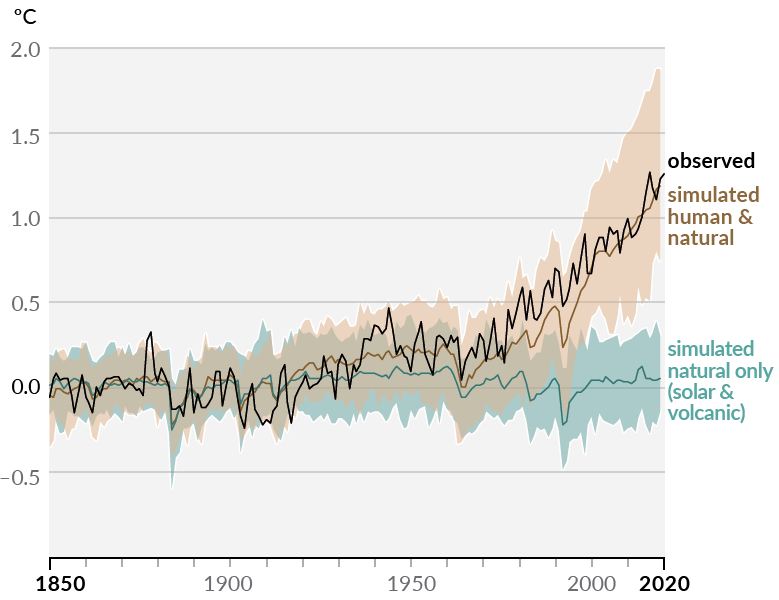
\includegraphics[width=0.6\textwidth]{figures/chapter1_figures/ipcc_fig1.png}
\end{figure}

There is absolutely no question that climate change is occurring. The black line in Figure \ref{ipcc1} displays the change in global temperatures since 1850. The average global surface temperature of the 21st century is 0.99$^\circ$C warmer than the global surface temperature from 1850 to 1900 \citep{ipcc1_summary}. While finding global temperatures is more complicated than a simple average, refuting that the planet is warming amounts to questioning whether or not thermometers actually measure the temperature. The Earth is warming, and even though we cannot go outside and immediately see this, it is still an empirical reality. 

There also no question that climate change is driven primarily by human activity. The tan series in Figure \ref{ipcc1} are simulated results using both human and natural drivers of climate, and the green series are simulated results using only natural drivers of climate. These simulations comes from leading climate models which are heavily reviewed by the scientific community. Natural factors alone cannot explain the rise in global temperatures. Only when we incorporate the impact of humans into climate models does the observed warming make any sense. 

As intelligently crafted as these climate models are, they are remarkably complex. The complexity of these models makes it difficult to understand why the scientific community knows humans are responsible for the recent climate change. Before looking at how scientists attribute the changes in the climate to different factors that have the potential to influence climate, first we look at the possible causes for the climate to change. 

Climate does not change without reason. The energy that warms the Earth and controls the climate comes from the Sun. The Sun covers half of the Earth in radiation at any given time. The atmosphere and Earth reflect about 30\% of this radiation back into space. The atmosphere absorbs 19\% of this radiation, and the surface of the Earth absorbs the remaining 51\%. When absorbed by the Earth's surface, the surface emits infrared radiation, or heat. Surface heat accounts for some of the planet's warmth, but most of this actually comes from the atmosphere \citep{csi}. When the surface emits infrared radiation, this moves out into the atmosphere. Certain particles sometimes absorb this infrared radiation and send it back to the surface. We call these particles \emph{greenhouse gasses}. Greenhouse gases keeps some heat energy from leaving the planet, similar to how a blanket keeps some heat from leaving your body. This heat is not inevitably trapped on the planet, but allows the same energy to be reabsorbed by the surface before attempting to leave the atmosphere again.

The planet's global temperature is stable when the radiative energy that coming into the Earth is equal to the radiative energy that the Earth emits back into space. When the radiative energy that comes to Earth is greater than the radiative energy the leaves Earth, then this surplus energy causes warming \citep{noaa}. This imbalance that causes changes in global temperatures is called \emph{radiative forcing} or \emph{climate forcing}.

There are several major factors that impact radiative forcing: solar irradiation, volcanic eruptions, land use, aerosols, and greenhouse gases \citep{SINGH202179}. \emph{Solar irradiation} refers to the power the Sun gives to the Earth on a per unit of land basis (W/m$^2$). One important factor affecting solar irradiation is the Earth's orbit and rotation. The Earth rotates on a 23.5$^\circ$ axis currently, but over the course of millennia, the tilt of this axis changes. This change in rotation and the subsequent climatic changes are known as the Milankovitch cycles. These cycles also incorporate slight changes in the Earth's orbit that make it more elliptical, bring the planet closer to the Sun during certain periods. While this does affect climate, it does so over the course of thousands of years rather than decades. Other fluctuations from the Sun have the potential to create radiation forcing and changes in the climate over somewhat shorter periods of time. For instance, reduced solar output is a leading explanation of the period of cooler climate in Europe and North America from the early 14th century to the early 19th century, an event known as the Little Ice Age \citep{little_ice}.

Land use, volcanic eruptions, and aerosols affect the planet's \emph{albedo}, the reflectivity of the planet. Recall that the Earth reflects about 30\% of the radiation from the sun. This percentage can change based on the presence of reflective and absorbent features on the surface and in the atmosphere. Some of this reflection occurs at the Earth's surface. White ice reflects radiation, while the black pavement of roads absorbs the Sun's radiation, emitting back the heat or infrared radiation. Agricultural land is generally more reflective than dark forests. Changes in land use like these can affect how much energy the surface absorbs or reflects, and consequently change the planet's albedo and climate. 

Another way to change the Earth's albedo and climate is through aerosol concentrations. Aerosols are small solid or liquid particles in the atmosphere that are can influence cloud cover and the Earth's albedo. Around 90\% of all aerosols in the atmosphere come from natural sources including dust, sea salt, and  wildfire ash. Humans emit the remaining 10\% of aerosols. Burning coal releases sulfur dioxide and driving cars releases fine particulate matter, both aerosols. Aerosols affect climate in two ways: (1) the direct effect of either absorbing or reflecting radiation in the atmosphere, and (2) cloud formation \citep{gfdl}. Most aerosols reflect light and have a cooling effect, with the notable exception of black carbon. Black carbon absorbs light and can be particularly destructive if it coats glaciers, turning these reflective surfaces black. This is the direct effect of aerosols. The second, indirect effect of aerosols is in the creation of clouds. Clouds require aerosols in order to form. Additional aerosols in the atmosphere make cloud formation easier and can even lengthen the lifespan of a cloud. This additional cloud cover reflects radiation and keeps the surface cooler. Unfortunately many common aerosols like sulfur dioxide are dangerous for human health and create acid rain in large concentrations. 

Volcanic eruptions can also influence the planet's albedo. It is true that volcanic eruptions emit greenhouse gases like carbon dioxide. However, volcanic greenhouse gas emissions are less than one percent of all anthropogenic emissions \citep{usgs, gerlach2011volcanic}. The suggestion that higher concentrations of carbon dioxide in the atmosphere are the result of volcanic eruptions rather than human activity is utterly false. Volcanic eruptions can often have a cooling effect on the climate (negative radiative forcing). These eruptions send large quantities of sulfur dioxide, an aerosol, into the troposphere. This creates large, and long-lasting clouds that reflect solar radiation and raise the Earth's albedo. 

\begin{figure}
	\caption{Current Carbon Dioxide Concentrations are Unprecedented \citep{noaa1} \label{noaa1}}
	\centering
	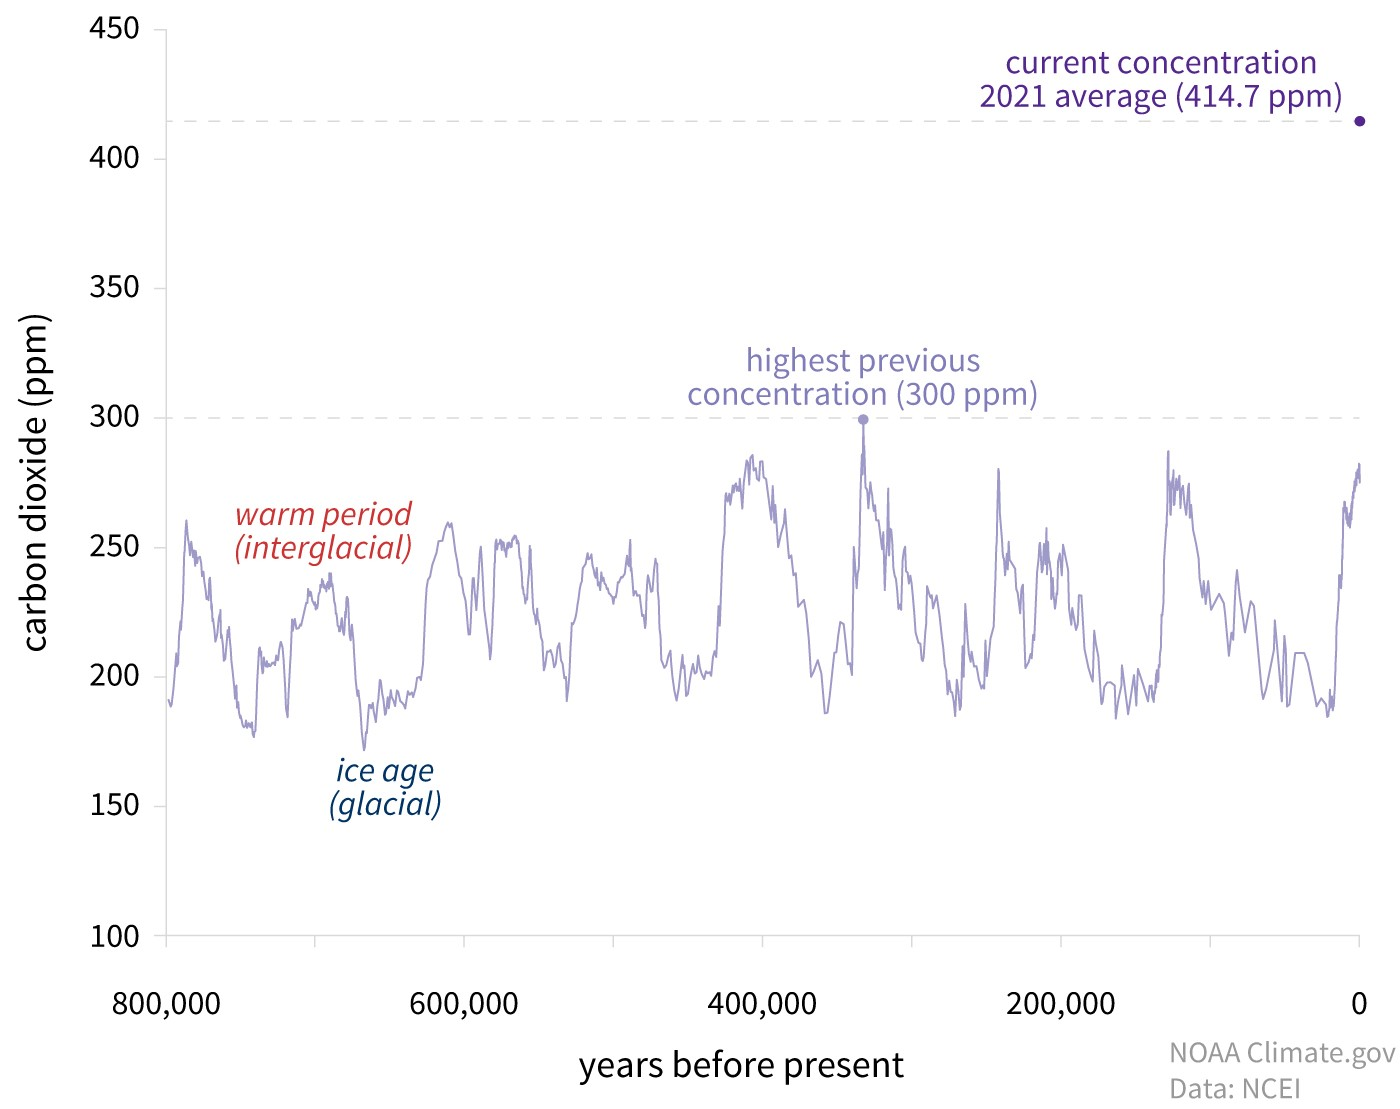
\includegraphics[width=0.7\textwidth]{figures/chapter1_figures/co2_noaa.jpg}
\end{figure}

Lastly, greenhouse gases can create radiative forcing. Higher concentrations of greenhouse gases make it more likely that any infrared radiation emitted on the planet's surface will be re-absorbed by the atmosphere and continue to heat the surface. The most important and common greenhouse gas is water vapor. Water evaporates from the surface, enters the atmosphere, absorbs heat from the planet, and keeps this heat around the surface. We know from the water cycle that the quantity of water vapor in the atmosphere is a function of the current temperature. For water to evaporate, it requires some external warming. For this reason we do not see radiative forcing from water vapor---any warming that occurs as the result of additional water vapor is attributable to the radiative forcing that caused the there to be more water vapor. Water vapor is an accelerator for the warming effect of other greenhouse gases.

The most recognized greenhouse gas is carbon dioxide or CO$_2$. Carbon dioxide makes up the bulk of all human-induced greenhouse gas emissions and, other than water vapor, is the most prevalent greenhouse gas in the atmosphere. Figure \ref{noaa1} shows the concentration of carbon dioxide in the Earth's atmosphere over the previous hundreds of thousands of years. In all this time, the concentration of carbon dioxide in the atmosphere never exceeded 300 parts per million (ppm). In 2020, the atmospheric concentration of carbon dioxide reached 412.5 part per million. Historically, the increase in carbon dioxide is practically instantaneous, and this result is completely attributable to humans. Natural flucuations have played out for hundreds of thousands of years---what we see today is unprecedented and undoubtedly the result of human activity, not natural causes. Elevated concentrations of greenhouse gases can keep additional infrared radiation around the surface of the Earth, warming the world. The next section takes a closer look at greenhouse gas emissions in the US and globally. 

\begin{figure}
\centering
\caption{Warming is Driven by Human Activity \citep{ipcc1_summary}\label{ipcc2}}
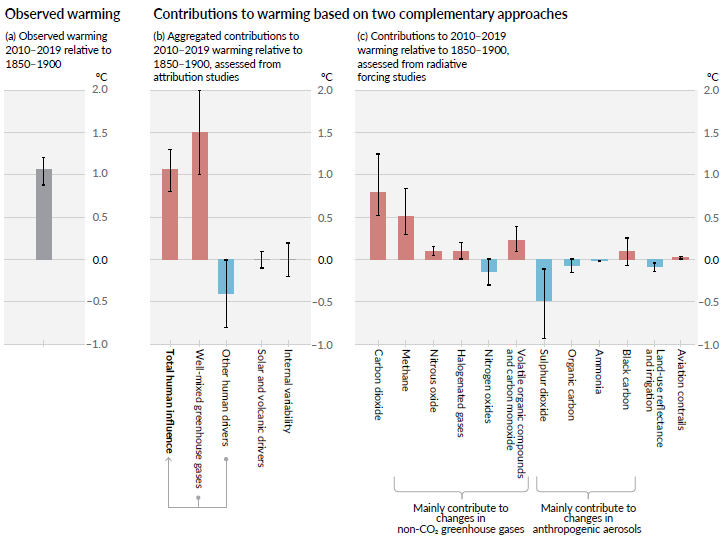
\includegraphics[width=\textwidth]{figures/chapter1_figures/ipcc_fig2.png}
\end{figure}

These various sources, solar irradiance, land use, aerosols, volcanic eruptions, and greenhouse gases, represent a comprehensive list of the factors that could possibly change global temperatures like we have seen them change. From here, scientists can measure how each of these factors have changed over the period we have seen warming. Incorporating some physical constants, researchers calculate the radiative forcing of each of these factors. Figure \ref{ipcc2} displays the results of these radiative forcing studies. This makes it remarkably clear that humans are responsible for climate change. 

Natural radiative forcing from solar drivers, volcanic activity, and internal variability is not perceptible. Historically, this is not surprising. The planet has never warmed so quickly---why would natural forces suddenly cause warming unlike any other time in history? Instead we see that warming is attributable to increases in greenhouse gases like carbon dioxide, methane, nitrous oxide, and others. This warming is partially offset by increasing concentrations of aerosols. Furthermore, we know that humans are responsible for the large increases in these greenhouse gases. We call the climate change caused by humans, rather than natural forces, \emph{anthropogenic climate change}.

If we are not convinced by the calculations of scientists and researchers, observational evidence can still demonstrate the human-origins of climate change. The planet is warming, but not quite the entire planet. The lowest level of the atmosphere that humans inhabit has warmed, but the upper layers of the atmosphere that absorb radiation from the Sun have not \citep{C2ES}. If climate change was the result of some change external to the Earth, then the stratosphere would warm as well. Without any warming in the stratosphere, we know that the warming must occur from activity on the Earth's surface. Natural activities on the surface like volcanic eruptions cannot account account for changes in temperature. These factors have largely remained unchanged over the period of warming we have already encountered, and often make such small contributions to shifts in global climate that we cannot seriously attribute climate change to these factors. Simple deduction leaves human activity as the culprit of the climate crisis. The Fourth National Climate Assessment makes the summation of all these scientific observations clear:
\begin{quote}
``Global average temperature has increased by about 1.8°F [1.0$^\circ$C] from 1901 to 2016, and observational evidence does not support any credible natural explanations for this amount of warming; instead, the evidence consistently points to human activities, especially emissions of greenhouse or heat-trapping gases, as the dominant cause." \citep{nationalar4}
\end{quote}


\subsection{Greenhouse Gas Emissions: Structure \& Trends}

Anthropogenic greenhouse gas emissions drive climate change. Carbon dioxide, methane, and nitrous oxide dominate greenhouse gas emissions in the US and globally. Florinated gases, also called F-gases, make up a non-negligible proportion of greenhouse gas emissions in the US, and are growing at an alarming rate.

Not all greenhouse gases are created equal. Some greenhouse gases remain in the atmosphere longer than others and absorb more infrared radiation from the Earth than others. Greenhouse gases may also react and create different greenhouse gases in the atmosphere, which themselves can have different warming effects. To improve the accounting of greenhouse gases, researchers standardize the varied warming effect of these greenhouse gases through a measure called global warming potential (GWP). GWP measures the warming effect of other greenhouse gas emissions relative to the warming effect from a ton of carbon dioxide. For instance, in the IPCC's 5th Assessment Report, methane has a GWP of 28, meaning that a ton of methane emissions has the same warming effect as 28 ton of carbon dioxide. This metric then leads to carbon dioxide equivalent emissions, a standard unit of account for different greenhouse gas.

\begin{table}
\centering
\caption{Global Warming Potential (GWP) by Greenhouse Gas \label{gwptable}}
\begin{tabular}{l c C{4cm} C{4cm}}
	\hline
	& & \multicolumn{2}{c}{IPCC Calculated GWP  over 100 Years}\\	
	\cline{3-4}
	Gas Name & Chemical Formula & Fourth Assessment Report & Fifth Assessment Report \\ 
	\hline
	Carbon dioxide & CO$_2$ & 1 & 1 \\
	Methane & CH$_4$ &25 & 28 \\
	Nitrous oxide & N$_2$O & 298 & 265\\
	HFC-134a & CH$_2$FCF$_3$ &1,430 & 1,300\\ 
	HFC-23 & CHF$_3$ & 14,800 & 12,400 \\
	Nitrogen trifluoride & NF$_3$ & 17,200 & 16,100\\
	Sulfur hexafluoride & SF$_6$ & 22,800 & 23,500\\
	\hline
\end{tabular}\\
\smallskip

\raggedright \footnotesize
Original data from \cite{forster2007changes} and \cite{ipcc_ar5_forcing}. Table adapted from \cite{gwp_table}.
\end{table}

Table \ref{gwptable} lists the GWP for the most common greenhouse gases and a handful of F-gases as calculated under the IPCC's Fourth and Fifth Assessment Reports. Carbon dioxide is always one because it is the standard unit. Methane has a shorter atmospheric lifespan than carbon dioxide, but absorbs much more energy during this time. The agriculture industry accounts for the largest share of methane emissions, followed closely by the mining and processing of fossil fuels.\footnote{\url{https://www.epa.gov/ghgemissions/overview-greenhouse-gases}} Nitrous oxide emissions occur almost entirely from agriculture, particularly from the application of fertilizers and other soil management practices. These emissions linger in the atmosphere longer than methane and absorb heat better than carbon dioxide. The IPCC's  latests estimates indicate one ton of nitruos oxide equates to 265 tons of carbon dioxide. F-gases like HFC-134a (the most common hydroflorocarbon in the atmosphere), HFC-23, nitrogen trifluoride, and sulfur hexafluoride are rare. These gases emerged to replace chlorofluorocarbons following the Montreal Protocol. While these gases do not have quite the same ozone-destroying effect of their predecessors, they can have huge GWP in even small quantities. They tend to remain in the atmosphere for a much longer time and absorb far more energy than more common greenhouse gases. For this reason, F-gases are also often called high GWP gases.

\begin{figure}
\caption{US Greenhouse Gas Emissions 1990--2019\label{ghg1}}
\centering
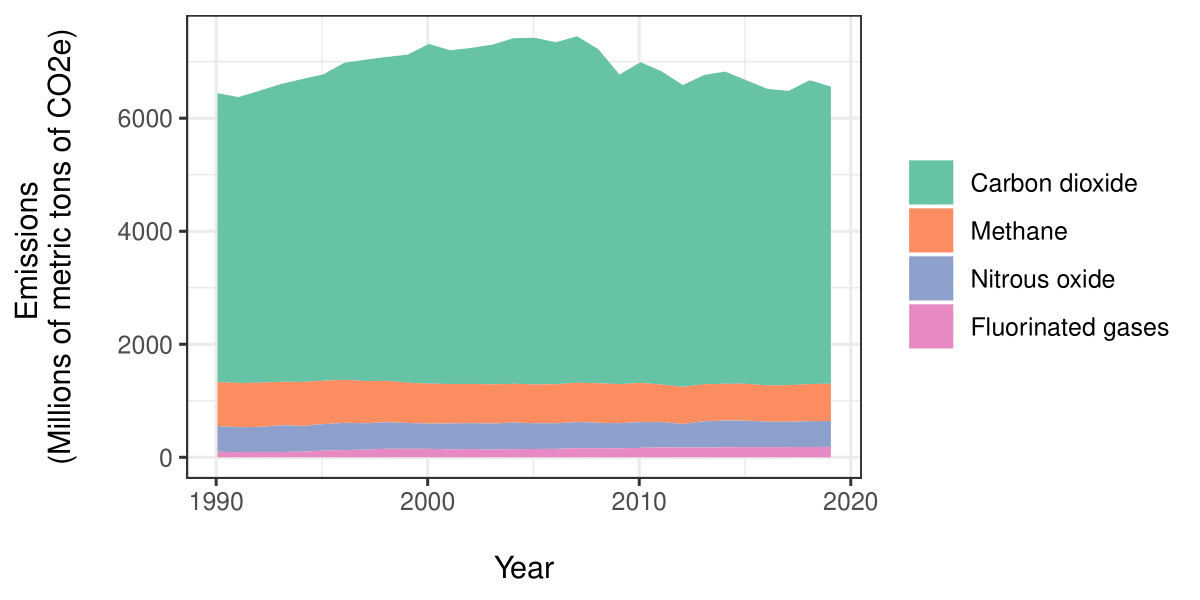
\includegraphics[scale=1]{figures/chapter1_figures/ghg_stacked.png}
\end{figure}

When we put all anthropogenic emissions into a common measurement, carbon dioxide equivalent, then we can compare greenhouse gas emissions and accurately evaluate the composition of greenhouse gases and the threat of certain gases relative to others. Figure \ref{ghg1} plots total greenhouse gas emissions (in millions of metric tons of carbon dioxide equivalent, CO$_2$e) in the US from 1990 to 2019 by the offending greenhouse gas. First, US greenhouse gas emissions have fallen over the past ten years. Second, it is clear why there is so much emphasis on carbon dioxide. Carbon dioxide makes up a clear majority of all anthropogenic greenhouse gas emissions in the US. Most of the recent reductions in greenhouse gas emissions are attributable to falling carbon dioxide emissions. Although they still make up just sliver of emissions, F-gases have seen the most growth over the period, up 86.3\%. 

\begin{figure}
\caption{US Greenhouse Gas Emissions by Economic Sector 1990--2019 \label{ghgeconomic}}
\centering
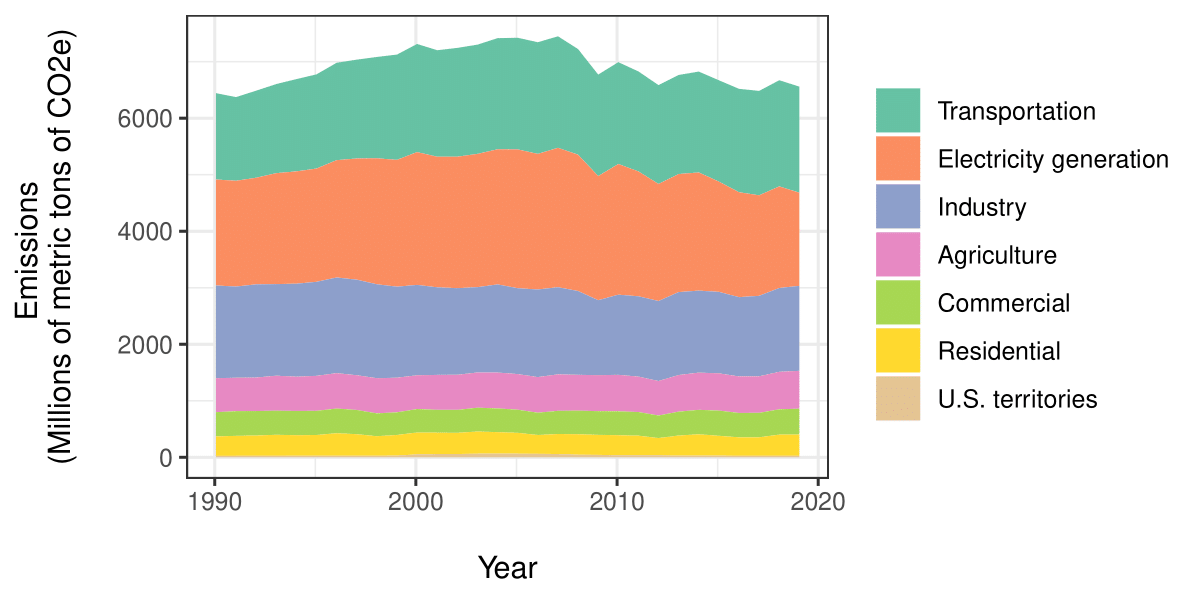
\includegraphics[scale=1]{figures/chapter1_figures/ghg_economic.png}
\end{figure}

Where then are these greenhouse gases coming from? One way to answer this question is by looking at greenhouse gas emissions by economic sector. Figure \ref{ghgeconomic} plots the greenhouse gas emissions of major US economic sectors in carbon dioxide equivalent from 1990 to 2019.  The emissions reductions from electricity generation and industry have driven the most recent decline in greenhouse gases. Transportation has consistently been the largest source of emissions, making up 28.6\% of all US greenhouse gas emissions in 2019. Electricity generation makes up a slightly smaller share with a clearer path to zero emissions through the expansion of renewable electricity generation and other low-carbon intensity fuel sources. Industrial greenhouse gas emissions have fallen by just about 8\% since 1990, and 22.9\% of all US emissions were from industry in 2019. The agriculture industry contributed 10.2\% of all US emissions in 2019. Commercial and residential emissions occur mostly from burning fossil fuels to heat buildings and homes. Together, these accounted for 12.7\% of all emissions in 2019. 

\begin{figure}
\caption{US Greenhouse Gas Emissions by Inventory Sector 1990--2019}
\centering
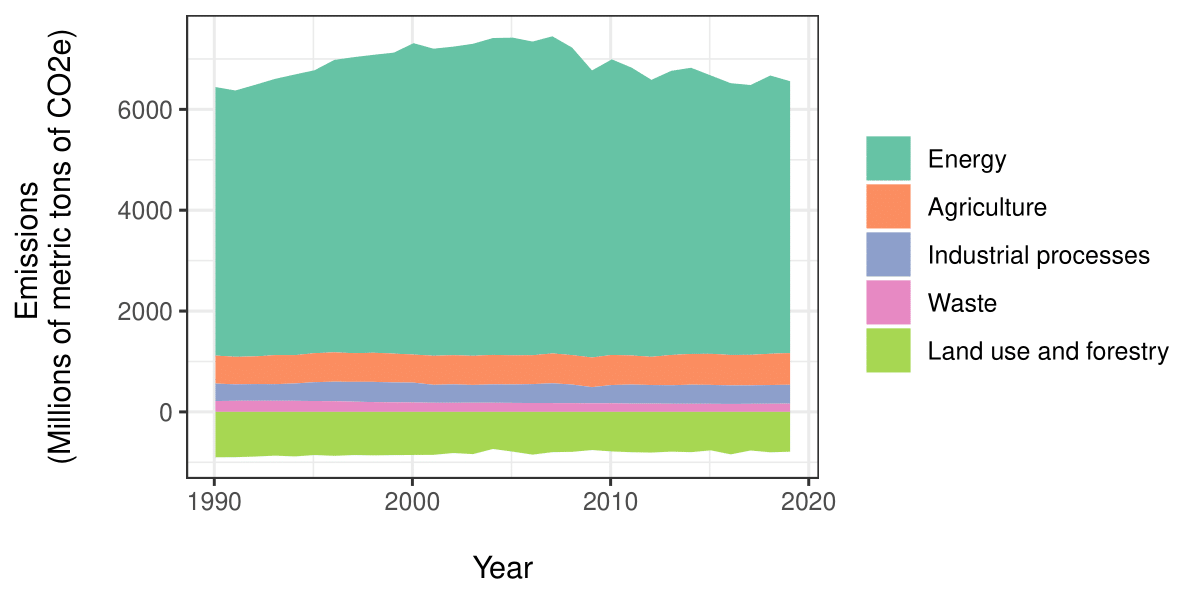
\includegraphics[scale=1]{figures/chapter1_figures/ghg_inventory.png}
\end{figure}

The US also reports greenhouse gas emissions by inventory sector, which considers the physical sources that create and remove emissions. This can be more useful than looking greenhouse gases by economic sector if different economic sectors create emissions for similar reasons. Indeed, we see that energy generation commands the majority of greenhouse gas emissions across economic sectors. Energy makes up 82\% of gross greenhouse gas emissions in the US. This is driven by the burning of fossil fuels, releasing carbon that was trapped in the ground into the air. Agriculture and waste both make meaningful contributions, mostly through methane and nitrous oxide emissions. Hydroflorocarbons and other high GWP gases are responsible for a considerable portion of emissions that occur during industrial processes. The EPA also reports data on the nations carbon sink. Carbon dioxide cycles naturally through the environment, emitted into the atmosphere by decomposing organic matter and reabsorbed by plants life. This natural carbon sequestration creates the carbon sink. Forestry and other plant life remove emissions from the air and store them, a flow of greenhouse gas emissions out of the atmosphere. For the US to reach net zero greenhouse gas emissions, this carbon sink must be equivalent to all other greenhouse gas emissions. 

\begin{table}
\caption{US Electricity Generation by Source \label{ele_gen_source}}
\centering
\begin{tabular}{l C{3cm} C{3cm}}
\hline \hline
Energy source & Billion kWh &	Share of total \\ 
\hline 
Fossil fuels & 2,427 & 60.6\% \\
\qquad Natural gas &	1,624	& 40.5\% \\
\qquad Coal & 773 & 19.3\%\\
\qquad Petroleum	& 17 & 0.4\% \\
\qquad Other gases & 11& 0.3\% \\
Nuclear & 790	& 19.7\% \\
Renewables & 792 & 19.8\% \\
\qquad Wind & 338 & 8.4\%\\
\qquad Hydropower	& 291 &	7.3\% \\
\qquad Solar & 91 & 2.3\% \\
\qquad Biomass	& 56 & 1.4\% \\
\qquad Geothermal & 17 & 0.4\% \\
Other sources & 8 & 0.2\% \\
Total: All sources	& 4,007  & ---\\
\hline \hline
\footnotesize \raggedright Data from \cite{eia_report1}.
\end{tabular}
\end{table}

With electricity generation and energy broadly making up such a considerable portion of US greenhouse gas emissions, it is important to understand the composition of electricity generation by fuel source in the US. Table \ref{ele_gen_source} shows the fuels that drive US electricity generation. Fossil fuels make up the majority of electricity generation with 60.6\% of all electricity coming from fossil fuels. Natural gas is the single largest fuel source for US electricity generation, with more electricity from natural gas than the next two most common fuels (nuclear and coal) combined. Natural gas burns much cleaner than coal; coal emits 95.74kg of carbon dioxide per million BTUs on average while natural emits 52.91kg of carbon dioxide per million BTUs.\footnote{British thermal units (BTUs) measure thermal energy. One BTU is the amount of heat energy required to warm one pound of water by one degree Fahrenheit. \url{https://www.eia.gov/environment/emissions/co2_vol_mass.php}} Still, Figure \ref{ghgeconomic} shows that despite the low emissions intensity of natural gas relative to other fossil fuels, it is still a fossil fuel that produces significant emissions. Fuels with low carbon intensities, like nuclear and renewables, make up the remainder of electricity generation, around 40\% of all US generation.

Climate change and excess greenhouse gas emissions might be a much simpler problem to address if they were unique to the US. They are global problems, and while the US is a major emitter of greenhouse gases, it is not the only nation with significant emissions. Figure \ref{global_ghg} shows the greenhouse gas emissions by country from 1990 to 2016. China is the largest producer of greenhouse gases, followed by the US. India and the European Union currently put similar quantities of greenhouse gases in the atmosphere, but are trending in opposite directions. As India develops, its emissions are growing, while Europe's emissions are falling. We see here that just a few countries, particularly the US and China, make up a significant portion of all greenhouse gas emissions. In these countries, emissions reductions are especially important. 

\begin{figure}
\caption{Global Anthropogenic Greenhouse Gas Emissions 1990--2016 \label{global_ghg}}
\centering
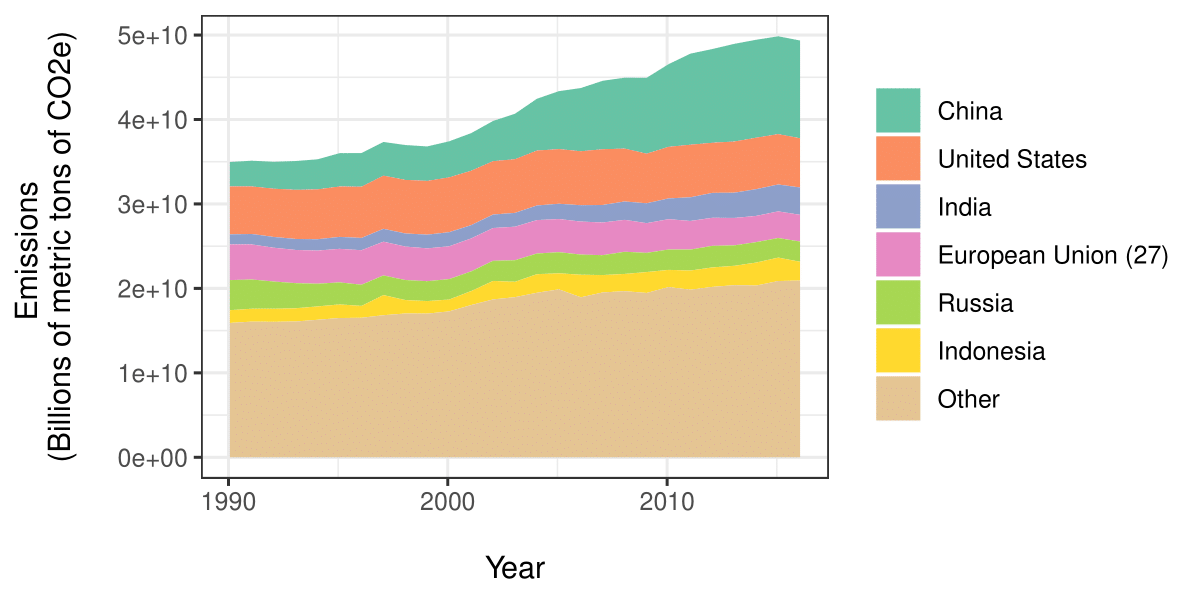
\includegraphics[scale=1]{figures/chapter1_figures/ghg_international.png}
\end{figure}

Although the US is a major contributor to global greenhouse emissions, it is not the largest (second place, woohoo). When we consider greenhouse gas emissions in per capita terms though, the situation in the US seems even more imperiled. Figure \ref{global_ghg_cap} looks at greenhouse gas emissions per capita for the leading greenhouse gas contributors. The US far outpaces other developed nations. Notably, the US has more than double the greenhouse gas emissions per capita as China. The US stands out on the global stage as in terms of wealth, size, and apparent inability to reduce its greenhouse gas emissions.

\begin{figure}
\caption{2016 Greenhouse Gas Emissions per Captia of Leading Emitters \label{global_ghg_cap}}
\centering
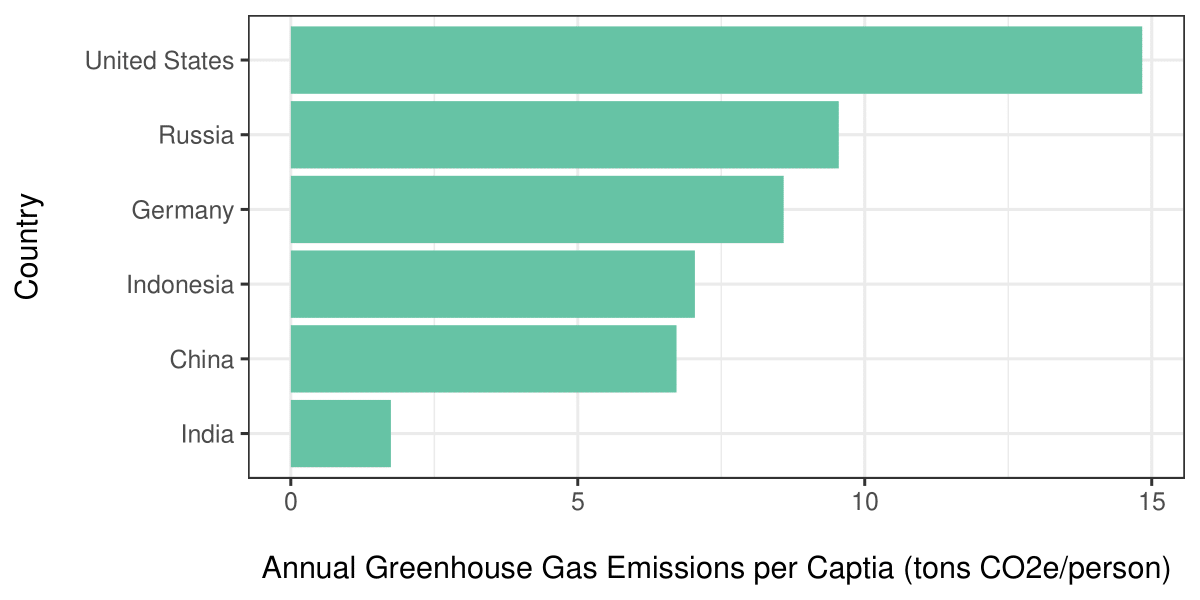
\includegraphics[scale=.9]{figures/chapter1_figures/ghg_cap.png}
\end{figure}


\subsection{The Impacts of Climate Change}

The previous sections have demonstrated that human activity, particularly the burning of fossil fuels, is responsible for climate change. Before we start designing policy to reduce greenhouse gas emissions, we first need to understand how climate change affects us today and could affect us in the future. In this section, we discuss some of the major impacts of climate change.

First though, we should discuss how we estimate future damages from climate change. 

The overarching approach 

Before we can estimate how climate change will affect the world in the future, we have to start with assumptions about what the world will look like in the future. Given this, we then 






The goal of climate impact studies is to estimate how emissions today and in the future will lead to a climatic scenario and then estimate how that climatic scenario will ripple through different ecosystems, communities, and economies. Economists often take this a step or two further, and try to put all of the costs (and benefits) of climate change into economic terms and then tie these prices into present terms. This gives the foundation for the the social cost of carbon [CITATION, https://www.rff.org/publications/explainers/social-cost-carbon-101/]. For our present purposes we do not need to relate all of these impacts back into prices, so we will omit a more detailed description of the social cost of carbon for now. 

The inputs to these climate impact models are known as emissions pathways. Despite the name, emissions pathways do not truly map out different emissions scenarios, but different concentrations of greenhouse gases alongside certain socioeconomic assumptions. A simplified emissions pathway might assume a certain time series of greenhouse gas concentrations, human population, and GDP over the century. The Intergovernmental Panel of Climate Change (IPCC) has standardized two collections of emissions pathways: Representative Concentration Pathways (RCPs) and Shared Socioeconomic Pathways (SSPs).\footnote{Often you might see something such as ``RCP$_{4.5}$" or ``SSP$_{8.5}$." The numeric subscript indicates the amount of radiative forcing the emissions scenario creates by 2100. For instance, RCP$_{4.5}$ will lead to 4.5 W/m$^2$ of radiative forcing---a measure of the average energy absorbed by the planet. Similarly, SSP$_8.5$ creates 8.5 W/m$^2$ by 2100, and is often used as the ``do nothing" response to cliamte change [CITATIONS, AR6 SPM]} Climate models then assume these scenarios and map out what the climate looks like over the course of the century using these 

% - Something about General Circulation Models (GCMs?)?
% - What are the CMIP things?

Process-based models suffer in in important ways. First, they are computationally intensive. 



While these process-based models create the backbone of impact estimates, economists often opt to use simpler method for mapping climatic outcomes to quantitative impacts called damage functions. Damage functions are reduced-form estimations of the relationship between climate variables (e.g. average surface temperatures) and impact variables of interest (e.g. mortality rates). That is, damage functions do not attempt to explain the complex systems that give rise to these damages and focus instead on just explaining aggregate impacts. For instance, [CITATION] create straightforward damage functions for the US by using process-based impact models to generate estimates of climate change impacts (in monetary terms) under a variety of climate scenarios. Then they use OLS to estimate the relationship between surface temperature measurements and the monetary value of climate change impacts. The estimated model is a damage function, mapping changes in surface temparatures to impacts. Damage functions like this and many others provide useful tool in a variety of applications, especially in calculating the social cost of carbon. 

\cite{auffhammer2018quantifying} notes that perhaps the greatest difficulty in using damage functions to map climatic scenarios into physical impacts is accounting for adaptation. Although it would be much easier to assume that people and businesses . \cite{auffhammer2018quantifying} uses the example of an air conditioner. Suppose we are interested in the impact of a changing climate on electricity use. We expect there to be more hot days, meaning that people will run their air conditioners more frequently and use more electricity to do so. This response on the intensive margin is measurable; we have the data to estimate how people use their air conditioners differently when it is warmer outside. The extensive margin cannot be realiably measured. 
We do not have reliable measurements for how many more people will purchase and use air conditioners after decades of sustained warming.\footnote{A promising but limited approach to studying climate change adaptation is by estimating how people have adapted to climate changes in the past. For instance, [CITATION, Drunkenmiller] are using historical aerial photographs of Western Africa to study land use and migration changes that occurred as a result of drought during the mid-twentiwth century.}

Admittedly, there is a considerable amount we still do not know about the impacts of climate change. Truthfully, we are not exactly sure how the estimated 3.3 to 3.6 \emph{billion} people who are highly vulnerable to climate change will adapt [CITATION]. Will hundreds of millions of people living in some of the most impoverished corners of the planet seemlessly migrate en masse to places with more hospitable climates over the course of just a few decades? 

What we do know is that today, our best estimates indicate that the impacts of climate change are frightening. 

In the preceeding subsections, we look at the

The IPCC outlines five major ``reasons for concern" regarding climate change:
\begin{enumerate}
	\item Unique and threatened systems
	\item Extreme weather events
	\item Distribution of impacts
	\item Global aggregate impacts
	\item Large-scale singular events
\end{enumerate}
These represent some of the most important risks that we face from climate change. 

% intramarginal vs. extramarginal

\subsubsection*{Unique \& Threatened Systems}

While many systems---both natural and social---face steep challenges from climate change, some of these face complete ruin. Many of the most vulerable systems are endemic. Endemism refers to species, cultures, and resources that are restricted to specific geographic areas. [CITATION] In a changing climate, systems that are tied to specific regions and climates risk extinction if they cannot plausibly adapt. This includes the extinction of species whose habitats are destroyed by climate change, 
the death of indigenous cultures that are highly dependent on the climate, and the destruction of historical artifacts and landmarks. Unfornately in each of these cases, the affected system cannot is unique and we could not replace it for the remainder of human existence. These kind of consequences do not fit well into standard economic understanding of sustainability. \footnote{*Talk about an economic definition of sustainability from Romer, and why it might not be able to capture some of the threats of climate change well.*}


\subsection{The Impacts of Ambient Air Pollution}

\textit{Forthcoming}.


\subsection{A Review of Air Quality Disparities}

\textit{Forthcoming}.



%%%%%%%%%%%%%%%%%%%%%%%%%%%%%%%%%%%%%%%%%%%%%%%%%%%%%%%%%%%%%%%%%%%%
%\subsection{The Impact of Climate Change}
%
%At this point we have covered why we know climate change exists, why we know humans are responsible for climate change, and what the composition of greenhouse gas emissions look like. We have to to justify why anyone should care about climate change though. Here, we take a brief and high-level examination of the impacts of climate change. If I had to summarize the magnitude of climate impact estimates by even just the end of the century, I would probably say that they lie somewhere in between pretty bad to borderline apocalyptic. 
%
%Admittedly, the impacts of climate change on natural ecosystems and society are not understood quite as well as the causes of climate change. This gap in knowledge is closing as we collect new data on the impact of the climate change we have already seen. The IPCC summarizes these impacts in its Fifth Assessment Report in five ``reasons for concern." These reasons for concern relate to:
%\begin{enumerate}
%	\item Unique and threatened systems
%	\item Extreme weather events
%	\item Distribution of impacts
%	\item Global aggregate impacts
%	\item Large-scale singular events
%\end{enumerate}
%
%There are certain physical elements of the natural and built environment that are unique and irreplaceable. Losing these due to climate change poses a significant cost for all future generations. For instance, warming waters threatens coral reefs. With sustained and substantial warming, the world's coral reefs could be permanently destroyed. Many important historical sites are located in low-lying coastal areas threatened by rising sea levels from climate change. Climate change has the power to permanently destroy many of the ecosystems we cherish and other culturally significant creations.
%
%Extreme weather events pose the greatest This includes a greater frequency of severe but short-lived weather events, like tornadoes or monsoons. More concerning is are sustained heat-stress events. As Freddy's mom from iCarly once said, ``when temperatures get too high, the elderly will start to die" (a rather creepy but fitting rhyme). Elevated temperatures can induce cardiovascular events, particularly in vulnerable populations like the poor, elderly, and those who work outside. Sustained events like this can trigger droughts and resulting in famine. Higher humidity can bolster mosquito populations and allow blood-borne infectious disease to spread easier. Extreme and sustained events like these pose serious challenges to public health.
%
%Related to this, impacts tend to fall most severely on populations who are already at the greatest disadvantage. Some of this is simply due to geography. Climate predictions for the African continent are sickening. Much of this is due to adaptation costs. When it is 110$^\circ$F outside, the well off do not just sweat---they run their air conditioners on full blast. This is not true of the global poor, who cannot afford to pay to adapt to rising temperatures, and instead suffer the heat and risk death. 
%
%Global impacts on natural life and the economy are not well understood, but what we know is not reassuring. The economic impacts of climate change will become much more apparent as concentrations of greenhouse gases increases. That is, the economic damages from climate change are increasing at an increasing rate with the concentration of greenhouse gases. There is some additional concern about low-probability, highly dangerous climate change-induced events. 
%
%\begin{figure}
%	\caption{Climate Change Damages by Income \& Climate \citep{carleton2020valuing} \label{cil1}}
%	\centering
%	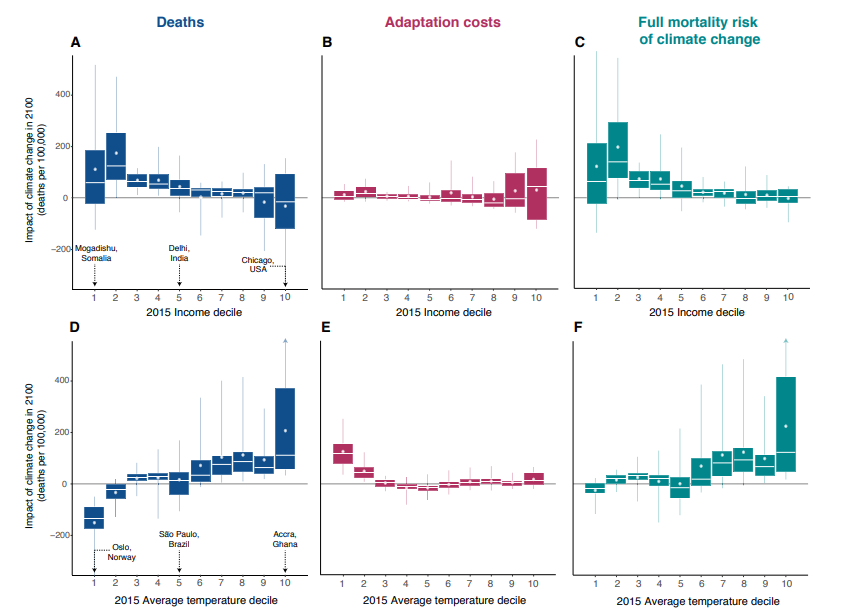
\includegraphics[width = \textwidth]{figures/chapter1_figures/cil_dist.png}
%\end{figure}
%
%\begin{figure}
%	\caption{The Climate Change Mortality Rate \citep{carleton2020valuing} \label{cil2}}
%	\centering
%	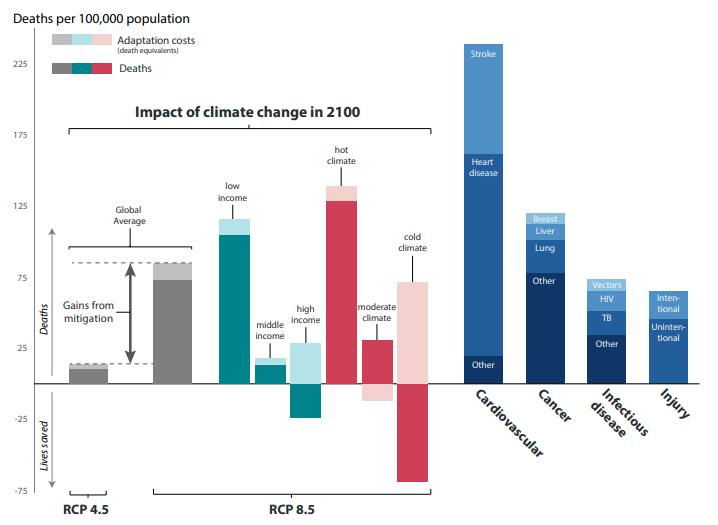
\includegraphics[width = 0.8\textwidth]{figures/chapter1_figures/cil_mortal.png}
%\end{figure}
%
%Figures \ref{cil1} and \ref{cil2} depict estimates of moralities by end of the century from climate change induced events. These summarize many of the most important takeaways from the impacts of climate change. Those who live in poor and warm areas will suffer the most from climate change. The mortality rate from climate change is comparable to the mortality rate of other leading causes of death. Overall, the situation climate change poses by just the end of the century is extremely grim and warrants sweeping action.
~

\newpage
\section{Designing Climate Policy}

\subsection{A Case for Economic Analysis in Climate Policy Design}

This chapter shifts the discussion from describing climate change to describing the policy tools available to address climate change. Before delving too far into this topic, it is worth contemplating why the economics discipline has any role at all in the design of climate solutions. While the physical sciences have alerted the world to the destructive potential of climate change and occupy a central role in developing the abatement technologies needed to mitigate climate damages, economically-motivated actors have largely been the perpetrators of the greenhouse gas emissions responsible for climate change. It seems reasonable then to question why economics deserves a place in designing climate solutions. There is a purported tension between mitigating climate change damages and protecting the economy---a tension that I discuss in greater detail later in this chapter. This belief that the economy and environment are fundamentally at odds might lead to the impression that elevating the environment must be done without regard to the economy. If nothing else, the cost-benefit analysis that underlies much of the economics discipline feels inappropriate when it comes to environmental issues. After all, why should we care about money when the fate of the planet is at risk?

The objective of this section is to address these concerns and motivate the use of economic analysis in climate policy design. First and foremost, it is important to establish that economic analysis should not and cannot hope to address climate change without other disciplines. There is a tremendous need for scientific research into technical solutions with the potential to reduce greenhouse gas emissions. In the International Energy Agency's plan to achieve net zero emissions by 2050, currently available technologies can only sustain abatement through 2030. By 2050 only half of the technology needed to reduce emissions is currently on the market. The agency estimates that governments worldwide will need to immediately invest over \$90 billion into key areas of research and development like electrification and carbon capture technologies---areas that currently receive only about \$25 billion in research funding \citep{ieareport}. Not only does the world need to efforts of the physical sciences to address climate change, but economists do for their own work as well. As discussed in section \ref{scc_section}, the damage functions economists use to estimate the costs of climate change necessarily rely on the physical sciences to build the underlying climate models. Clearly, economic analysis alone cannot guide climate policy design. 

Still, physical science alone cannot hope to address climate change without the perspective of the social sciences. 




% \begin{figure}
% 	\centering
% 	\caption{Climate Cynicism}
% 	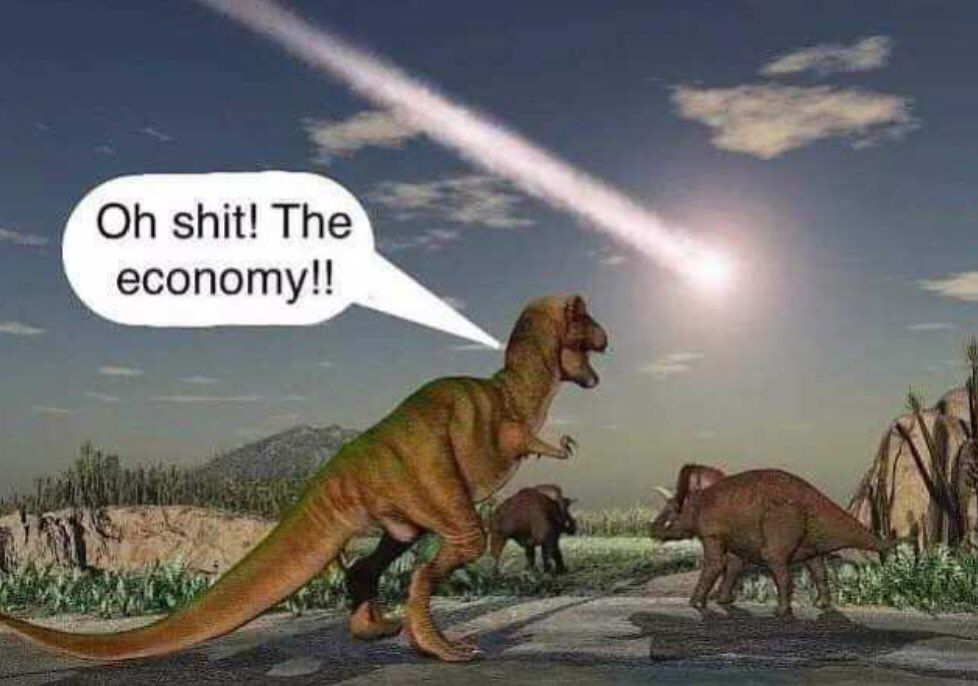
\includegraphics[scale=0.2]{figures/chapter2_figures/dino.jpg}\\
% 	%\footnotesize This is a rough draft so I'm allowed to have this
% \end{figure}

As a discipline
Amongst the social sciences,


First, economic tradeoffs exist whether or not we acknowledge them, and these tradeoffs are not always simple. 

Consider an impoverished community with a coal-burning power plant. The plant emits sulfur dioxide into the air, which can lead to respiratory issues. But if the plant is to reduce its emissions and continue operating, the cost of electricity will likely rise and hurt the already poverty stricken community. Workers at the plant may lose their careers. Though troublesome, there is a tradeoff here between public health and poverty alleviation. 

For the sake of example, consider a low-income, credit-constrained government. To keep this example simple, suppose the government can invest its publicly borrowed funds into either converting the nation's coal generation into clean, renewable generation or into expanding public education. Though troublesome, there is an apparent tradeoff in this scenario between improving the environment and improving access to education---both worthy goals with the potential to benefit future generations. \cite{nordhaus2019climate} makes this point more poignantly in his Nobel lecture:
\begin{quote}
	``However attractive a temperature target may be as an aspirational goal, the target approach is questionable because it ignores the costs of attaining the goals. If, for example, attaining the 1.5°C goal would require deep reductions in living standards in poor nations, then the policy would be the equivalent of burning down the village to save it."
\end{quote}

\textbf{This isn't just some highly contrived example\ldots}

Economists generally try to quantify these competing interests and place them in terms of a common unit, the dollar.\footnote{Expressing costs and benefits in terms of dollars is often  convenient though not necessary. For instance, in Figure \ref{cil_mortality}, \cite{carleton2022valuing} express climate change adaptation costs not in dollars, but in terms of ``statistical lives."} The question of climate mitigation costs and benefits may seem irrelevant or even unethical to some observers, but assigning numeric costs to climate inaction provides a consistent and open framework to



Second, money is the primary concern of firms engaged in emissions producing activities. The economics discipline largely concerns itself with the incentives of both firms and consumers---incentives that if designed well, can lead to substantial emissions reductions. Money undoubtedly plays a role in determining whether or not people drive electric cars, manufacturers install smokestack scrubbers, and electric power producers build fossil fuel generators. Even if we concede that bringing the world down to net zero emissions is invaluable, public policy that does not systematically consider how firms and consumers will react risks failure. In a global crisis at the scale of climate change, the potential costs of this risk are substantial. 

Lastly, despite what some political pundits might propagate, the economic consensus is remarkably clear: climate change is a major threat that warrants significant action. In a 2021 survey of climate economists, 74\% said that climate change necessitates ``immediate and drastic action." Less than 3\% answered that either ``more research is needed before action is taken" or that climate change ``is not a serious problem" \citep{howard2021gauging}.\footnote{Another 24\% said that ``some action should be taken now" on climate change.} Although it may seem trivial to some, economists largely agree that the benefits of bold climate policy outweigh the costs. The economic perspective adds further credibility to the case for climate policy, particularly when much of the criticism lodged at climate action focuses on its cost. 

In summary, economics provides a quantitative and systematic approach to making potentially difficult decisions related to our relationship with the Earth's atmosphere and our environment. This is approach is not without its flaws, but it is one of many important perspectives. Not only does economic analysis allow us to consider the tradeoffs of specific policy proposals, but it provides theory and empirical techniques essential to identifying how firms and individuals will respond to policy. Climate economists predominantly agree that climate change urgently deserves bold public policy, a view that aligns with climate scientists and researchers at large. While physical scientific research can develop the technologies that permit emissions reductions, research in economics and other social sciences will be integral in the successful adoption of these technologies and related behavioral changes.


\subsection{An Economic Motivation for Climate Policy}

% The general approach advocated by policymakers begins by making the production of electric power less carbon intensive. This involves the familiar steps of switching from coal power plants, to wind and solar farms. This is called \emph{decarbonization} of the electric power grid. Simultaneously, policymakers need to transition energy-using activities to rely on electric power, rather than other forms of energy. Electric vehicles are the most popular push for electrification. Some greenhouse gas emissions are likely inevitable, so bringing the world to net zero emissions requires that those emissions are offset through increased carbon sequestration, the removal and storage of CO$_2$ emissions from the atmosphere. The tree is a simple carbon sequestration device, but difficult to use at the necessary scale. Carbon sequestration technology requires significant public investment, but unlike decarbonization and electrification, this does not need to involve many economic actors.

The first chapter established anthropogenic greenhouse gas emissions as the culprit behind climate change, but this still leaves open questions surrounding the social and economic motivations behind these emissions. Any public policy aimed at reducing greenhouse gas emissions must first reconcile with why those greenhouse gas emissions exist in the first place. Moreover, despite having established that economics as a discipline deserves a role in climate policy design, it is worth considering whether or not public policy is necessary to address climate change at all. The objective of this section is to fill in these holes and provide an economic interpretation for both why climate change happens and why climate change is not likely to improve in the absence of public policy. This section uses foundational elements of economic theory to answer two questions: (1) why do individuals and firms release greenhouse gases into the atmosphere, and (2) can we ``solve'' climate change without public policy? 

To the economist, climate change is the consequence of the \emph{universal} nature of greenhouse gas emissions. Greenhouse gas emissions  are a textbook example of an externality: a cost or benefit borne by an agent who is not involved in the economic transaction that creates the cost or benefit. Consider a driver with a gasoline-fueled car. Overall, burning gasoline creates greenhouse gas emissions that lead to anthropogenic climate change which would harm the average driver. The transaction between the driver and pump creates costs that are universal, borne by everyone on the planet, which are are externality by definition. When this driver buys and burns a gallon of gasoline in her car, she damages the climate by a non-negligible amount. In fact, a quick back-of-the-envelope calculation would suggest a central estimate for the cumulative damages associated with this gallon of gasoline of about \$1.64.\footnote{The \cite{epa2022greenhouse} finds that burning a gallon of gasoline in the average passenger vehicle creates 8887 grams of CO$_2$ emissions. Using a SCC of \$185 per tonne, as in \cite{rennert2022comprehensive}, this implies the social cost of burning a gallon of gasoline of 
$$\frac{8887 \text{g CO$_2$}}{1 \text{gallon gasoline}} \cdot \frac{1 \text{tonne CO$_2$}}{10^6 \text{g CO$_2$}} \cdot \frac{\$185}{1 \text{tonne CO$_2$}} \approx \frac{\$1.64}{1 \text{gallon gasoline}}.$$
Note also that this best thought of as a lower bound on true social damages, as this does not consider damages associated with the ambient air pollution emissions.} However, this cost is not borne by the driver alone, but distributed over the other eight billion people on the planet and even over the billions of people not yet born who will be affected by this decision in the future. Despite the additional or marginal damages from this gallon of gasoline of \$1.64, the climate damages that the driver faces herself for buying and burning this gallon of gasoline are effectively zero. If for instance, we simplified the situation to consider only damages that accrue to those eight billion people currently alive and assume that this driver experiences the average damages of all individuals, then her private cost of the associated emissions is approximately \$1.64/8 billion $\approx 0$. As a result, the price this driver pays for a gallon of gasoline is just the price at the pump. Because the driver's costs do not reflect the universal costs of her emissions, she will end up consuming more of this good than what would be socially optimal.

% For any individual driver, the impact of burning one more gallon of gasoline on the climate is entirely negligible, and the cost she incurs for that next gallon of gasoline is just the price she pays at the pump. Unfortunately, she is not the only person who incurs the costs of the induced climate change---so do the other eight billion people on the planet.\footnote{There are additional externalities here related to how this activity will affect future generations. The extraction of the oil for gasoline production prevents future generations from extracting and using that same unit of oil. Future generations will also feel the climate effect caused by present emissions. In both cases, the value of these damages are highly dependent on the assumed discount rate. These are known as intertemporal externalities \citep{keohane2016markets}.} 
% However, she does not face the burden of climate change damages incurred by all other people caused by her driving. These costs are external to the driver when she chooses how much gas to put in her car or what car to buy in the first place. 

\begin{figure}
	\caption{Market for an Emissions-Intensive Good \label{mkt_ei_good}}
	\centering
	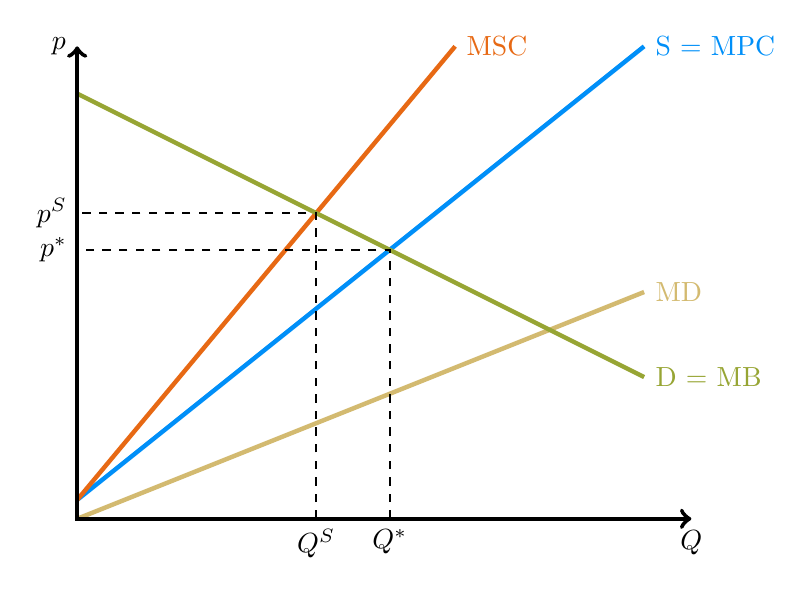
\begin{tikzpicture}[scale=0.6]
		\draw[ultra thick, color1, domain=0:12] plot (\x, {.8*\x + .4}) node[right]{S = MPC};
		\draw[ultra thick, color6, domain=0:12] plot(\x, {.4*\x}) node[right]{MD};
		\draw[ultra thick, color3, domain=0:8] plot(\x, {1.2* \x + .4}) node[right]{MSC};
		\draw[ultra thick, color2, domain=0:12] plot (\x, {-.5*\x + 9}) node[right]{D = MB};
		\draw[thick, dashed] (6.615, 0) node[below]{$Q^*$} -- (6.615, 5.692) -- (0, 5.692) node[left]{$p^*$};
		\draw[thick, dashed] (5.059, 0) node[below]{$Q^S$} -- (5.059, 6.471) -- (0, 6.471) node[left]{$p^S$};
		\draw[ultra thick, <->] (0,10) node[left]{$p$} -- (0,0) -- (13,0) node[below]{$Q$};
	\end{tikzpicture}
	\fignote[1]{Figure depicts a standard market for an emissions-intensive good, such as gasoline. In the figure, $p$ denotes the price of the good, $Q$ denotes the quantity of the good, D denotes demand, S denotes supply, MB denotes the marginal benefit associated with consumption, MPC denotes the marginal private cost associated with production, MD denotes the marginal damages stemming from the associated greenhouse gas emissions at a given quantity, and MSC denotes the marginal social cost---the sum of the marginal damages and the marginal private cost. In this case, we assume that marginal damages are increasing in $Q$, reflecting the accelerating disruptions caused by elevated greenhouse gas concentrations in the atmosphere.}
\end{figure}

Figure \ref{mkt_ei_good} depicts a generalized version of this situation diagrammatically through the market for an emissions-intensive good. As in any standard market, the market for an emissions-intensive good relates the quantity of this good ($Q$) to its price ($p$). The effective components of the market are the downward-sloping demand curve (D), and the upward-sloping supply curve (S). Here, consumers demand the good such that the price they will be willing and able to pay for an additional unit of the good is equivalent to the additional or marginal benefit (MB) they receive from consuming it, hence why D $=$ MB. Similarly, producers supply the good such that the price they will be willing and able to sell an additional unit of the good at is equivalent to its additional or marginal private cost (MPC), hence why S $=$ MPC. Together, the demand and supply for the emissions-intensive good lead to an equilibrium price and quantity of $p^*$ and $Q^*$ respectively. 

Outside of the market though, the production and consumption of the emissions-intensive good produces greenhouse gas emissions, which lead to climate change and associated damages to others. The upward-sloping marginal damages curve (MD) depicts the cost of these emissions for each additional unit of the good. As in the previous example, these damages accrue to society at large, but not to the individual involved in the transaction. The marginal social cost (MSC) considers the full scope of costs associated with the emissions-intensive good, summing the marginal private costs and the marginal (social) damages. Total welfare in the market is maximized when the marginal social cost is set equal to the marginal benefit, an unreached equilibrium at $Q^S$ and $p^S$. Note that for an emissions-intensive good, the socially-optimal price is higher than the equilibrium price and the socially-optimal quantity is less than the equilibrium quantity. That is, the market will under-price and over-produce an emissions-intensive good. The concept of externalities provides an economic explanation for why society creates excessive greenhouse gas emissions that lead to climate change. 

It is worth considering then why---if the atmosphere is in fact so valuable---there is no market for clean air. Modern economic theory classifies goods according to two criteria: rivalry and excludability.\footnote{\cite{ostrom2010beyond} reviews the historical development of the four goods commonly used today. The seminal paper \cite{samuelson1954pure} moved the discipline away from just private goods and described a public good, introducing the excludability criterion. Although \cite{hardin1968tragedy} popularized the concept of rivalrous goods, club goods were first formally introduced in \cite{buchanan1965economic} and open-access goods were first formally introduced in V. Ostrom and E. Ostrom (\citeyear{ostrom1977public}).} A good is rival if one agent's consumption of the good inhibits another agent's consumption of the good, or is non-rival if one agent's consumption of the good does not inhibit the consumption of any other agents. Concert tickets, for example, are a rivalrous good---one person holding a ticket prevents another person from holding that same ticket. A good is excludable if it is reasonably easy to prevent someone from using it. Video subscription services are excludable, as a service can always prevent a person from accessing the service if, for instance, he stops paying his bill. If we accept the double dichotomies of a good being either rival or non-rival and excludable or non-excludable, then these criteria lead to four types of economic goods: private goods (excludable and rival), public goods (non-excludable and non-rival), open-access goods (non-excludable and rival), and club goods (excludable and non-rival).\footnote{Here I choose to use the term ``open-access good'' rather than ``common-pool resource,'' a term more common in work such as \cite{ostrom1990governing}. The intention of this choice is to clarify the non-excludability of this class of goods. A common-pool resource might be shared by a group of agents, but still excludable to others outside of this group. For instance, \cite{ostrom1990governing} considers a community forest in the Swiss Alps where the right to fell timber in the community forest was restricted to certain land owners who could prevent others from purchasing land that would grant them the timber rights. The term ``open-access good'' more clearly describes a good that is available to any interested actor but still rival (e.g., using the swing set at a public park).} These good matrix in Figure \ref{goods} summarizes these four types of goods.

\begin{figure}
	\caption{A Taxonomy of Goods}
	\label{goods}
	\centering
	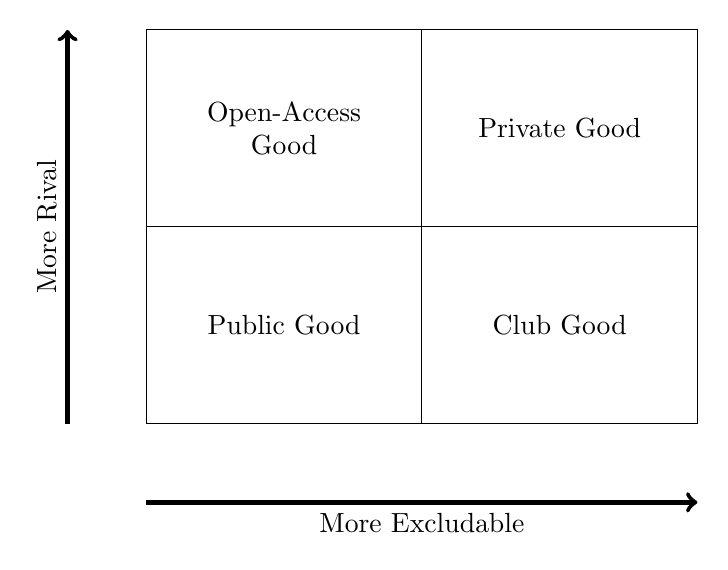
\begin{tikzpicture}[scale = 0.5]
		\draw (0,0) rectangle (7,5) node[pos=.5] {Public Good};
		\draw (7,5) rectangle (14,10) node[pos=.5] {Private Good};
		\draw (0,5) rectangle (7,10) node[pos=.5, text width = 2.5cm, align=center] {Open-Access Good};
		\draw (7,0) rectangle (14,5) node[pos=.5] {Club Good};
		\draw[ultra thick, ->] (0,-2) -- (14, -2) node[pos =.5, below]{More Excludable};
		\draw[ultra thick, ->] (-2, 0) -- (-2, 10) node[pos =.5, above, rotate=90]{More Rival};
	\end{tikzpicture}
	\vspace{1em}
	\fignote[1]{The goods matrix depicts the four main types of goods: private goods (excludable and rival), public goods (non-excludable and non-rival), open-access goods (non-excludable and rival), and club goods (excludable and non-rival). Although these are cannonically presented in four categories, the excludability and rivalry of goods is best thought of as taking place on a continuum.
	}
\end{figure}

A clean atmosphere is firmly a public good. There is no way to prevent people from benefiting from a healthy atmosphere with greenhouse gases at a level that supports climate stability, and one person's benefit does not infringe on another's. By the same virtue, greenhouse gas emissions are a public bad. No individual can exclude herself from climate change, and one person's climate damages do not prevent someone else from also experiencing those same damages. 

Defining a clean atmosphere as a public good provides a grounded explanation for why socially efficient greenhouse gas emissions abatement is unlikely to occur in the absence of public policy. All public goods struggle to find buyers. This lack of buyers is not necessarily because few people are willing and able to pay for the public good, but because these people do not have the proper incentives that would motivate them to actually buy into the public good. To see this, suppose there are two cities $A$ and $B$ on either side of a lake that is currently polluted and covered in algae blooms. Both cities benefit from the clean water in the lake through greater aesthetic appeal, higher property values, and increased ecotourism. As we have described it, clean water in the lake is a public good. Neither city can exclude the other from enjoying the clean water and one city's enjoyment of the clean water does not inhibit the other city from enjoying the clean water. 


adapted from \cite{keohane2016markets} 




\begin{figure}
	\caption{Market for a Public Good \label{mkt_public_good}}
	\centering
	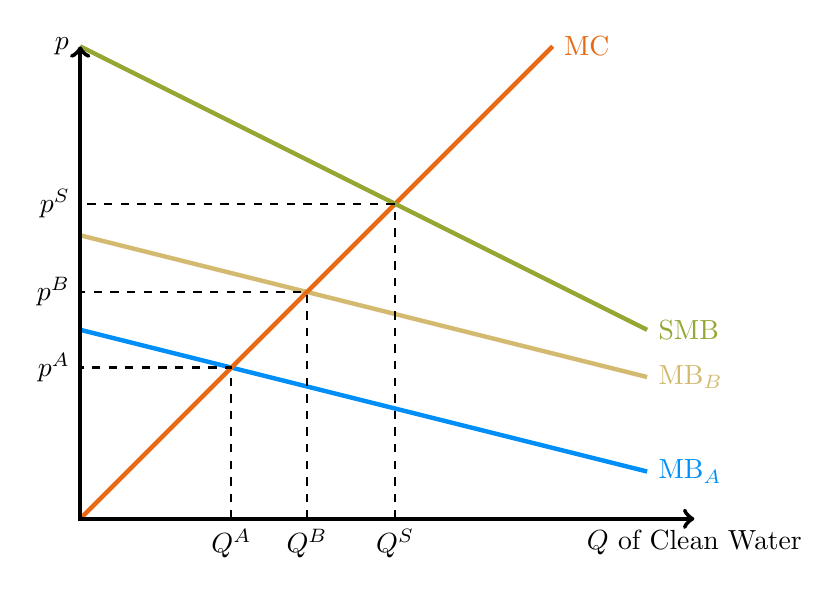
\begin{tikzpicture}[scale=0.6]
		\draw[ultra thick, color1, domain=0:12] plot (\x, {4 - .25*\x}) node[right]{MB$_A$};
		\draw[ultra thick, color6, domain=0:12] plot(\x, {6 - .25*\x}) node[right]{MB$_B$};
		\draw[ultra thick, color3, domain=0:10] plot(\x, {\x}) node[right]{MC};
		\draw[ultra thick, color2, domain=0:12] plot (\x, {10 - .5*\x}) node[right]{SMB};
		\draw[thick, dashed] (3.2, 0) node[below]{$Q^A$} -- (3.2, 3.2) -- (0, 3.2) node[left]{$p^A$};
		\draw[thick, dashed] (4.8, 0) node[below]{$Q^B$} -- (4.8, 4.8) -- (0, 4.8) node[left]{$p^B$};
		\draw[thick, dashed] (6.667, 0) node[below]{$Q^S$} -- (6.667, 6.667) -- (0, 6.667) node[left]{$p^S$};
		\draw[ultra thick, <->] (0,10) node[left]{$p$} -- (0,0) -- (13,0) node[below]{$Q$ of Clean Water};
	\end{tikzpicture}
	\vspace{1em}
	\fignote[1]{Figure depicts a market for an emissions-intensive good, such as gasoline, based on Figure 5.4 in \cite{keohane2016markets}. In the figure, $p$ denotes the price of the good, $Q$ denotes the quantity of clean water, MC denotes the marginal cost of clean water, MB$_A$ denotes the marginal benefit of clean water to city $A$, MB$_B$ denotes the marginal benefit of clean water to city $B$, SMB denotes the social marginal benefit which is the sum of MB$_A$ and MB$_B$. The figure demonstrates that even in the smallest of public good provision situations, the equilibrium production of the public good be less than the socially efficient.}
\end{figure}



With this discussion of public good provision in mind, consider again whether or not it is possible to ``solve'' climate change---in the sense limiting of limiting---in the absence of public policy. 


Even with domestic climate policy, this of course still leaves room for free riding at the global level. However, with a public policy focus in mind, the relevant actors are no longer individuals but entire nations. This change drops the number of relevant actors from billions to just dozens, making the prospect of cooperation far more likely. Currently, international cooperation has been mostly limited to voluntary climate pledges like the defunct Kyoto Protocol or the Paris Climate Agreement, where the compliance and enforcement of commitments is ambiguous at best. There are however other, more enforceable options at the international level to promote cooperation and prevent nations from shirking on their climate obligations. The most prominent of these approaches is likely the idea of a ``climate club,'' popularized by \cite{nordhaus2015climate}. A climate club is a group of nations that imposes trade penalties on other nations that do not fulfil their climate obligations, providing some incentive for nations to create policy that reduces their emissions profiles. Climate clubs are already beginning to emerge informally through the implementation of the European Union's recently revised Carbon Border Adjustment Mechanism (CBAM), which levies trade restrictions in Europe against imports from nations with relatively emissions intensive production processes. I save a more through discussion of Border Carbon Adjustments (BCAs) for later in the chapter. 


For the sake of simplicity, assume that all technology needed to attain net-zero emissions and stablize the concentration of greenhouse gases in the atmosphere was commercially available. Even if this was the case, 



Overall, when a good is non-excludable, it is difficult to create an incentive structure that motivates individuals who value the public good to contribute to its provision. The field of mechanism design studies these incentive structures, as called ``mechanisms,''  with the intent of motivating individuals to reveal their private value for a public good and contribute this value to its provision. \footnote{See Chapter 7 of \cite{fudenberg1991game} for the authoritative treatment on the application of mechanism design to public good provision problems.} These mechanisms are mathematically complex, and ultimately always rely on a social planner to implement and enforce


Economists often use the classic prisoners' dilemma game to model a public good contribution game. 

All agents have a strictly dominant strategy to not contribute towards the public good, provided that they would prefer to not contribute to the public good and not receive it than finance the public good individually. A coal-burning power plant wants to prevent climate change damages, but preventing these damages will require sweeping action from around the world. It could not successfully mitigate climate change damages by itself, and even if it could, the costs involved would far exceed its benefits. If other actors choose to take aggressive action on climate change, then making serious abatement efforts costs the coal plant but provides no benefit. In either case, the plant is better off doing nothing. The universal, non-excludable nature of the benefits of climate change mitigation fails to create the proper incentives for individual actors to take action.\footnote{The rivalry of goods tends to be less important than their excludability in environmental contexts. \cite{hardin1968tragedy} famously considered the example of an English pasture to show that agents will overexploit non-excludable but rival goods, leading to the collapse of the natural system, provided the agents have no institutions that can enforce cooperation. For this reason, the excludability is the primary concern in the environmental and climate settings.}

Absent any additional incentive, individual agents will fail to implement the necessary changes. In some instances, economic actors can in theory internalize the externality through bargaining, a result known as the Coase theorem \citep{coase1960problem}. This implies that in certain circumstances, private agents can resolve externalities without public policy. 

Climate change does 
For the Coase theorem to hold even theoretically, there must be enforceable property rights and transaction costs must be negligible. These transaction costs are often substantial, especially when dealing with many different actors and assessing compliance is difficult. Because climate change involves quite literally every person on the planet (and many more people not yet born), it suffices to say that serious efforts at curbing climate change cannot be made without government involvement. Further, Coasean bargaining may have potentially troubling distributional consequences. However, bargaining will likely play a pivotal role in any successful international climate agreements. In these contexts, we can consider how bargaining may be able to address climate change without an international government. Even this will require national governments to implement strong climate policy.

Putting these pieces together, individual firms and consumers will emit far too many greenhouse gas emissions as the costs they face do not reflect the greater societal costs of their actions. These same firms and consumers will fail to produce a cleaner atmosphere, a necessary public good, because they cannot exclude others from enjoying the benefit of a clean atmosphere. Without this ability to exclude, those willing to produce a cleaner atmosphere will not do so because individuals do not have an incentive to buy a cleaner atmosphere. Without buyers, there can be no market for a clean atmosphere. The market failure that leads to climate change is less of a market failure and much more of a market omission. The omission of the market for a clean atmosphere creates ragged, incomplete edges in adjacent emissions intensive markets. Finally, the scope of the problem is so large that resolution of climate change through private actors is not only impractical, but too costly to be increasing welfare.


Decades later, Elinor Ostrom critiqued this dichotomy in her landmark book \textit{Governing the Commons}, in which she documents many cases from around the world where non-government institutions have successfully sustained resources including grazing land, forests, and groundwater aquifers. In each of these cases, individuals and firms organized themselves in ``collective action" to protect natural resources. 

Could similar approaches like those Ostrom studies succeed in creating climate action? It is highly unlikely. Ostroms focus on open-access resources, where a healthy atmosphere is firmly a public good (alternatively, greenhouse gas emissions are a public bad). Much of their analysis is based on the rivalry of the resources and consequently does not translate well for reducing emissions. More importantly, some of the key features that allow these self-governance approaches to succeed are not met in the context of climate change. The systems Ostrom studies are primarily local and rely on mutual-monitoring and enforcement. Given the global nature of climate change and the invisibility of greenhouse gas emissions, it would be a tremendous leap to say that climate action is achievable through self-governance and collective action alone. 

In summary, economic theory posits that agents will produce excessive greenhouse gas emissions because they do not face the full social consequences of their economic activities. A safe and stable atmosphere is public good, and consequently, private agents do not have an incentive to abate their emissions. Without policy intervention, the resulting equilibrium outcome will 

Although non-policy options exist to internalize the externality (e.g., Coasen strategies) or cooperate towards more socially desirable outcomes (e.g., collective action strategies), the number of relevant parties means these are not serious alternatives to public policy. 

The next section briefly address the suite of policy available 


\subsection{The Structure \& Scope of Environmental Policy}

In Garrett Hardin's classic work ``The Tragedy of the Commons,"  he proposes two approaches to managing open-access resources: privatization and nationalization. The key in both cases is consolidating agents, who would otherwise experience the consequences of each others' actions but not their own, under one umbrella. That is, when there is only one party in charge, there is no room to free ride.\footnote{It is worth noting that an $N$-player ``Tragedy of the Commons'' game is functionally identical to an $N$-player Cournot game. This highlights how the market behavior of a monopoly ($N =1$), under-producing and over-pricing a good, can actually become socially desirable in the case of environmentally damaging goods, which are usually over-produced and under-priced. Privatization and nationalization of the commons both amount to granting a monopoly on a good.} Today, many environmental policies still fall into a dichotomy that parallels the dichotomy Hardin discussed: market-based policies and command-and-control policies. 




Just as privatization of the commons consolidates incentives by , 

market-based policies consolidate social 

Just as nationalization of the commons places the state as in charge 

Again, both market-based policies and command-and-control policies 







It is not surprising that current climate policy in the US predominantly resembles the dichotomy espoused by Hardin. This same dichotomy appears in US environmental policy as well.




The inevitability of the incentive-induced failure of private management of the climate crisis forces public policy. Still, there is a wide variety of tools available to policymakers for addressing environmental and climate issues. 
%Figure \ref{policies} highlights the major types of environmental policies using classifications adapted from \cite{keohane2016markets}. 
Analogous to Hardin's dichotomy, environmental policy typically falls into one of two categories: \emph{market-based policy} and \emph{command-and-control policy}. Command-and-control policies create changes by enforcing directives, while market-based policies make use of primarily financial incentives.






Command-and-control policies are what we would typically think of as environmental regulation. Here, government creates specific prescriptions to firms and possibly consumers. For this reason, command-and-control policy is also often called \emph{prescriptive policy}. Prohibition policies prevent actors from taking certain actions, like purchasing a piece of public land or disposing of a hazardous chemical. These typically appear in the management of public lands, like National Parks, Wildlife Refuges, and Forests. Often alongside prohibition is permission, where government may for instance lease National Forests to the logging industry or grant rights to a firm to drill for oil on state-owned land. In a loose sense, we might also classify any policy enforcement as a part of this category. Regulators may prohibit certain activities with prescribed punishments for violators. 

Another approach to regulating and protecting the environment is through standard setting. Standards are generally either \emph{technology standards} or \emph{performance standards}. Technology standards require firms to use specific technologies. Many coal-burning power plants must install smokestack scrubbers to prevent damaging chemicals from entering the lower atmosphere. Alternatively, performance standards do not specify specific technologies, but set bounds on the rate or total magnitude of an environmental impact. This could involve setting an emissions cap on an individual firm or car fuel economy standards, which indirectly govern the rate of carbon dioxide emissions per mile. The discipline lacks clear definitions for some of these classifications, and occasionally performance standards form a category between market-based and command-and-control policies. Technology standards provide the characteristic inflexibility of a command-and-control policy, but performance standards can provide somewhat more flexibility. 

Information tools can use a combination of both command-and-control and market-based policies. For instance, a mandatory eco-labeling program might require firms to display the carbon footprint of a good they sell. This a specific reporting requirement without a direct financial incentive attached to the policy. Still, consumers, seeing this information might change what and how many products they purchase. This creates secondary financial incentives for firms, similar to a market-based policy. Sometimes these programs are not mandatory, and firms  voluntary participate in labeling due to some financial incentive. Other times, there is no financial incentive for information disclosure, but regulators require disclosure regardless. This is the case in program's like the EPA's Greenhouse Gas Emissions Reporting Program. This program requires facilities that have potential high emissions to collect data and report on their greenhouse gas emissions.

Generally, market-based policies operate instead not by imposing specific rules, but instead by creating those essential but missing markets. Policymakers primarily do this through the two components of any market: price and quantity.  Price instruments are the traditional Pigouvian solution. When there is a market failure due to some externalitiy, we can internalize the externality by taxing or subsidizing a good so individual incentives will align with social incentive. Carbon taxes are a clear example of this strategy. There are costs of carbon dioxide emissions that do not appear in the prices of goods and activities that rely on these emissions. A carbon tax creates a financial incentive for firms and consumers to reduce their emissions. It also it flexible---no individual has to change her behavior, but continued emissions will come at a cost.  Analogous programs subsidize energy-efficient goods, providing a financial incentive to adopt durables that will use less energy and reduce emissions. 

Alternatively, policymakers might also use quantity-based instruments to create financial incentives. The typical example here is a cap-and-trade program, where policymakers require certain actors to own emissions permits or emissions allowances for every ton of their greenhouse gas emissions. Policymakers create a fixed quantity of these permits and can sell these to regulated firms. If firms were only allowed to keep these emissions allowances, then this would be equivalent to a performance standard. The key piece of the differentiation is the tradeable nature of these allowances. Under a cap-and-trade program, firms can buy and sell these emissions allowances from each other. This creates a market for allowances, which puts a price on emissions. Just like a carbon tax, the price of an emissions allowance creates a financial incentive for emissions abatement. Other programs outside of the reduction of greenhouse gas emissions make use of quantity-based instruments. For instance, Wetland Mitigation Banking in the US fixes a quantity of land for wetland conservation. Firms and farmers that wish to develop on existing wetland must offset this development by building or conserving a tract of wetland equivalent to the wetland they displace through development. 

% \begin{landscape}
% \begin{figure}
% \centering
% \caption{Taxonomy of Major Environmental Policies \label{policies}}
% \begin{tikzpicture}[grow = down, scale = 1, semithick]
% 	\footnotesize
% 	\tikzstyle{level 1}=[level distance=20mm,sibling distance=9cm]
%     \tikzstyle{level 2}=[level distance=5cm,sibling distance=4.5cm]
%     \tikzstyle{level 3}=[level distance=5cm,sibling distance=4.5cm]
        
%     \tikzstyle{s1}=[rectangle, rounded corners, text width=4cm, draw, inner sep = 5, fill = white, semithick,fill opacity = 0,text opacity = 1, minimum height = 4cm]
%     \tikzstyle{s1-mod}=[rectangle, rounded corners, text width=4cm, draw, inner sep = 5, fill = white, semithick,fill opacity = 0,text opacity = 0, draw opacity=0, minimum height = 4cm]
%     \tikzstyle{s2}=[rectangle, rounded corners, text width=6cm, draw, inner sep = 5, fill = white, semithick,fill opacity = 0,text opacity = 1]
%     \tikzstyle{s3}=[rectangle, rounded corners, text width=6cm, draw, inner sep = 5, fill = white, semithick,fill opacity = 0,text opacity = 1]
%     \tikzstyle{s4}=[rectangle, rounded corners, text width=4cm, draw, inner sep = 5, fill = white, semithick,fill opacity = 0,text opacity = 1]
    
	
% 	\node[s3, text centered]{Major Environmental Policy Options}
% 		child{node[s2, text centered]{Market-Based Policies}
% 			child{node[s1]{Price Tools
% 				\begin{itemize}
% 					\item Carbon taxes
% 					\item Border carbon adjustments
% 					\item Energy-efficiency subsidies
% 				\end{itemize}
% 			}
% 				edge from parent node[]{}}
% 			child{node[s1]{Quantity Tools
% 				\begin{itemize}
% 					\item Cap-and-trade
% 					\item Individual fishing quotas
% 					\item Wetland mitigation banking
% 				\end{itemize}							
% 			}
% 				edge from parent node[]{}}
% 			child{node[s1-mod]{I}
% 				edge from parent node[]{}}
% 			edge from parent node[]{}}
% 		child{node[s2, text centered]{Command-and-Control Policies}
% 			child{node[s1]{Information Tools
% 				\begin{itemize}
% 					\item Eco-labelling programs
% 					\item Green building certification
% 					\item Emissions reporting
% 				\end{itemize}
% 			}
% 				edge from parent node{}}
% 			child{node[s4]{Standard Setting}
% 					child{node[s1]{Performance-Based
% 							\begin{itemize}
% 								\item Minimum vehicle fuel efficiency standards
% 								\item Minimum ambient air quality standards
% 							\end{itemize}
% 						}
% 						edge from parent node[]{}}
% 					child{node[s1]{Technology-Based
% 							\begin{itemize}
% 								\item Smokestack scrubber requirements
% 								\item Sewage discarge equipment requirements
% 							\end{itemize}
% 						}
% 						edge from parent node[]{}}
% 				edge from parent node[]{}}
% 			child{node[s1]{Prohibition and Permission
% 				\begin{itemize}
% 					\item Endangered species protection
% 					\item Conservation land
% 					\item Drilling rights on public land
% 				\end{itemize}							
% 			}
% 				edge from parent node[]{}}
% 			edge from parent node[]{}};
% \end{tikzpicture}
% \vspace{.25cm}
% \begin{minipage}{0.8\textwidth}
% 	\footnotesize
% 	Classifications and examples developed from \cite{keohane2016markets}. 
% \end{minipage}
% \end{figure}
% \end{landscape}

So what policies are most effective? Economists tend to favor market-based over command-and-control approaches in many contexts for two primary reasons. First, market-based approaches are in a theoretical sense, cost-effective. That is, well-designed price and quantity tools can achieve environmental targets while minimizing the burden of regulation on firms and consumers. This seems somewhat ironic. Many environmental issues are fundamental examples of market failure, yet here the implication is that these same issues are best resolved inside of a market. \cite{keohane2016markets} perhaps say it best ``the problem is not that markets are so pervasive but that they are not pervasive \emph{enough}---that is, they are incomplete." Are economists naive to suspect that the same free-market principles that cause environmental issues can actually resolve them? The section that follows expands on this question by providing an example of why carbon taxes and cap-and-trade programs can be reasonably cost-minimizing, and some justification of why command-and-control policies are not. Later sections will address this empirically and show that market-based tools can be effective in resolving environmental and climate issues.

Second, market-based programs create incentives for firms to invest in research and development of new technologies with positive environmental impacts. Under a technology standard, firms have no interest in creating new technologies. Doing so would only impose additional and unnecessary costs on themselves. Additionally, if firms encountered technologies with the potential to reduce their environmental impact, they would have an incentive to hide it from public and particularly from regulators. Under a market-based approach, firms have a strong incentive to innovate new technologies. With a carbon tax, major innovations in abatement technology would allow firms to save on emissions costs, giving them a strong competitive advantage. If firms could anticipate future increases in the price of emissions, they might even make this investment even if the current emissions price was relatively low.
 
Despite the apparent merits of market-based approaches to environmental policy, price and quantity instruments are no panacea. One significant concern in many areas of environmental policy is enforcement. Natural resources are often incredibly large and it is difficult to monitor individual behaviors that relate to these resources. The earlier discussion on the cost-minimizing nature of these market-based approaches excludes any consideration of enforcement costs. What happens if we incorporate these costs into our analysis?

For instance, say we wanted to reduce bycatch on commercial fishing vessels. Bycatch is when fishers unintentionally catch sealife like dolphins or sea turtles instead of the fish they intended to catch. There are ways fisher can mitigate bycatch, like using specific kinds of nets that allow some species to escape.
Consider a market-based strategy to reduce bycatch, like taxing fishers for the non-targeted sea life that they catch and kill. If fishers followed this rule, the tax would be enough for many of them to adopt the technologies that would reduce bycatch. This would minimize the total costs incurred by fishers. Fishers who face high costs from reducing bycatch will barely reduce their bycatch as they would rather pay the tax. Fishers who face low costs from reducing bycatch will greatly reduce their bycatch as they would rather adopt new technologies than pay a tax. Of course, this assumes that there is perfect compliance and enforcement is costless. What kind of costs would be involved in enforcing a tax like this? Monitoring and taxing the bycatch of every commercial fisher in an area would be tremendously difficult and expensive. We do not have the technology to monitor every animal caught in every commercial fishing nets. Even there was a monitoring official on every large commercial vessel, there would be strong incentives for collusion. 

In situations where enforcement is incredibly costly, it may be more cost-effective to take a command-and-control approach that prescribes uniform policies across actors. In this example, it would much less expensive to require that commercial fishers use bycatch-reducing nets. Policymakers could incorporate this into existing procedures for commercial fishing licensing and even prevent the production and sale of more harmful nets. This policy would not be cost-minimizing for the fishers, but if the difference in enforcement costs was large enough, it may be more cost-minimizing to society as a whole. A technology standard, a command-and-control approach, seems more appropriate in this case.


\subsection{Environmental Markets: Carbon Taxes \& Cap-and-Trade}

To illustrate the theory behind these polices, consider the example of carbon taxes and cap-and-trade programs. The market missing in climate change is a market for emissions abatement. Figure \ref{abatement1} displays this market. The supply of emissions abatement is equivalent to the marginal abatement costs (MAC). Towards the left of the MAC curve are the low hanging fruit of abatement options.\footnote{Some empirical estimates of this curve suggest that this far portion of the MAC may actually be negative. That is, initial emissions abatement is achievable at a negative cost, as firms and individuals can often save money through energy-efficiency improvements. This is related to the energy-efficiency gap \citep[see][]{allcott2012there, gerarden2017assessing}.} As more abatement occurs, the technologies involved in abatement become more costly, and many of these require new research investments into technologies that are not yet available. 

Although there are private costs involved in emissions abatement, there are also social gains. These gains are equivalent to avoided climate change damages. Marginal damages increase with the quantity of emissions; the more emissions are already in the atmosphere, the greater the impact of an extra ton of CO$_2$. For this reason, the marginal benefits of abatement are decreasing. The first ton of CO$_2$ abated is responsible for the largest reduction in climate change damages, and any subsequent abatement is less effective at reducing damages. Abatement is a public good though, so despite the social benefits, no private agents are willing to pay for abatement. 

Market-based policies attempt to resolve this issue by using government to act as a ``demander" of abatement. It is impractical for policymakers to set a full demand curve for abatement, so instead policymakers can set clearer demand curves that will still bring the market to its true equilibrium. Namely, a policymaker can set a horizontal demand curve for abatement at $p^*$ or a vertical demand curve for abatement at $A^*$. These two options are identical in simple models of abatement as both lead to the socially optimal level of abatement. 

\begin{figure}
\caption{Creating a Market for a Public Good (or Bad)}
\centering
\subcaptionbox{The Market for Abatement \label{abatement1}}{
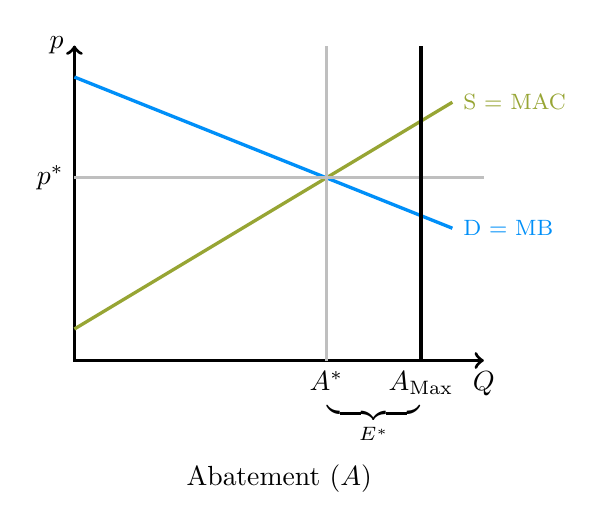
\begin{tikzpicture}[scale=0.4]
	\draw[very thick, <->] (0,10) node[left]{$p$} -- (0,0) -- (13,0) node[below]{$Q$}; 	
	\draw[very thick, color2, domain=0:12] plot(\x, {.6*\x + 1}) node[right]{\footnotesize S = MAC};
	\draw[very thick, color1, domain=0:12] plot(\x, {-.4*\x + 9}) node[right]{\footnotesize D = MB}; 
	\draw[very thick, lightgray] (8,0) node[below, black]{$A^*$} -- (8,10);
	\draw[very thick, lightgray] (0,5.8) node[left, black]{$p^*$} -- (13,5.8);
	\draw[very thick] (11, 0) node[below]{$A_\text{Max}$} -- (11, 10);  
	\node[below] at (6.5, -3) {Abatement ($A$)};
	\draw (9.5, -2) node{$\underbrace{~~~~~~~~~~}_{E^*}$};
\end{tikzpicture}
}
\hspace{.01cm}
\subcaptionbox{The Market for Emissions \label{emissions1}}{
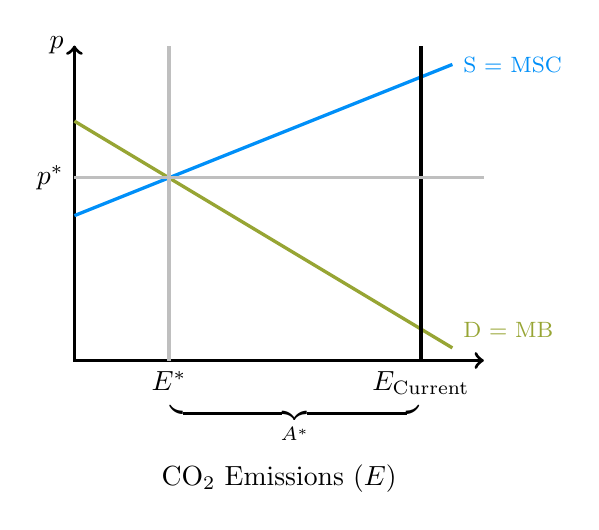
\begin{tikzpicture}[scale=0.4]
	\draw[very thick, <->] (0,10) node[left]{$p$} -- (0,0) -- (13,0);	
	\draw[very thick, color2, domain=0:12] plot(\x, {7.6 - .6*\x}) node[above right]{\footnotesize D = MB};
	\draw[very thick, color1, domain=0:12] plot(\x, {4.6 + .4*\x}) node[right]{\footnotesize S = MSC};
	\draw[very thick] (11, 0) node[below]{$E_\text{Current}$} -- (11, 10);
	\draw[very thick, lightgray] (3,0) node[below, black]{$E^*$} -- (3,10);
	\draw[very thick, lightgray] (0,5.8) node[left, black]{$p^*$} -- (13,5.8);	
	\node[below] at (6.5, -3) {CO$_2$ Emissions ($E$)};
	\draw (7, -2) node{$\underbrace{~~~~~~~~~~~~~~~~~~~~~~~~~~~}_{A^*}$};
\end{tikzpicture}
}
\end{figure}

The previous example framed market-based instruments from the perspective of creating a market for emissions abatement. 
%This approach highlights how government intervention can work to establish a market for a public good. Additionally, it makes use of the marginal abatement cost curve which is often relatively easy to estimate in practice. 
Although this framing is important and one that is often more convenient, the interpretation and public policy implications can seem counterintuitive. With government on the demand side, this would imply a policy where government pays polluters to abate, either promising a fixed rebate on each ton of emissions abated or by purchasing abatement until it reaches $A^*$. In this system, polluters would earn more revenue by through abatement. Major climate policy proposals do not include such massive payoffs to polluters, and rightly so; in the long run these economic profits would attract more firms to enter high-polluting industries and diminish the efficacy of policy. There may also be additional social costs if government reduces other expenditures or raises taxes in order to finance these payouts. 

The familiar policies focus on the inverse of the abatement market, the market for emissions. This market appears in Figure \ref{emissions1}. In this market, the government does not intervene to demand a public good, but to establish rights for and supply a public bad. The polluters derive their demand for emissions from their MAC curves---it represents the most polluters will be willing to pay for the right to send CO$_2$ emissions into the atmosphere rather than abate. The supply curve in this market is the marginal damage of emissions. This framing comes with a clearer interpretation. Here, policymakers impose a carbon tax---a charge of $p^*$ on each ton of CO$_2$ emissions. In equilibrium, this tax will lead to total emissions $E^*$. A cap-and-trade program program instead sets a vertical supply curve of emissions allowances, permits that give polluters the right to emit one ton of CO$_2$, at $E^*$. A key feature of these allowances is that they are tradeable between polluters. Although it is not necessary for government to sell or auction off emissions allowances, if government did, their equilibrium price would be $p^*$. 

The market for abatement and the market for emissions correspond. The difference between the maximum level of abatement and the equilibrium level of abatement is the equilibrium emissions, and the difference between the current level of emissions and the equilibrium level of emissions is the equilibrium abatement. The market price for emissions is the same as the market price for abatement. Framing market-based policy through the market for emissions has a more convenient interpretation relative to standard policy. However, because the prices and quantities are identical in both markets, economists often choose to frame market-based polices through the market for abatement rather than the market for emissions. This approach can be clearer when considering the cost-minimizing nature of market-based instruments.

\begin{figure}
\caption{Distribution of Allowances \label{dist_allowance}}
\centering
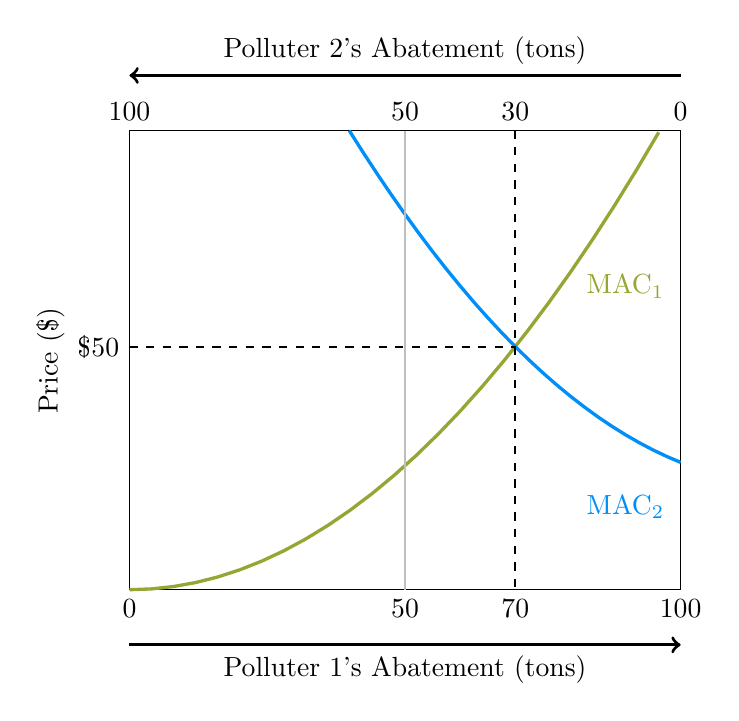
\begin{tikzpicture}[scale=0.7]
	\draw (0,0) rectangle (10,8.33);
	\draw (0,0) node[below]{0} -- (10,0) node[below]{100} -- (10,8.33) node[above]{0} -- (0,8.33) node[above]{100} -- (0,0);
	\draw[very thick, ->] (10, 9.33) -- (0, 9.33) node[pos=.5, above]{Polluter 2's Abatement (tons)};
	\draw[very thick, ->] (0, -1) -- (10, -1) node[pos=.5, below]{Polluter 1's Abatement (tons)};
	\draw[very thick, color2, domain=0:9.603] plot(\x, {.09*\x^2});
	\draw[very thick, color1, domain=3.988:10] plot(\x, {.1*(12-\x)^2 + 1.91}); 
	\draw[thick, dashed] (0,4.41) node[left]{\$50} -- (7,4.41);
	\draw[thick, dashed] (7,8.33) node[above]{30} -- (7,0) node[below]{70};
	\node[rotate=90, above] at (-1, 4.155) {Price (\$)};
	\node[color2] at (9, 5.5) {MAC$_1$};
	\node[color1] at (9, 1.5) {MAC$_2$};
	\draw[lightgray, thick] (5,0) node[below, black]{50} -- (5,8.33) node[above, black]{50};
\end{tikzpicture}
\end{figure}

It turns out that in our simple theoretical model of a cap-and-trade program with tradeable allowances, the original distribution of allowances is irrelevant to whether or not the policy achieves the emissions reduction cost-effectively. Suppose that there are just two polluters in our system, Polluter 1 and Polluter 2, each of whom currently has 100 tons in emissions. The assumed benevolent policymaker wants to cut emissions in half by setting a cap of 100 tons of emissions. Polluter 1 and 2 have marginal cost of abatement curves depicted in Figure \ref{dist_allowance}. Consider two alternative scenarios: (1) the policymaker sells allowances to the polluters, and (2) the policymaker gifts 50 (tradeable) allowances to each polluter. 

If the policymaker sells allowances to the polluters, then both polluters will purchase allowances up until the price of an allowance equals the cost of an additional ton of abatement. That is, each polluter will purchase the quantity of emissions allowances where the price of an allowance is equal to its marginal abatement cost. The demand for abatement is perfectly inelastic, so the equilibrium price will be where the sum of the quantities of abatement supplied by the polluters is 100 tons. Graphically, the total marginal abatement cost curve for the two polluters together is a horizontal summation of each individual marginal abatement cost curve. Figure \ref{dist_allowance} shows that at a price of \$50, the sum of the Polluter 1 and 2's abatement is 100 tons, the desired level of abatement. Total abatement costs are equal to the area under each abatement curve from 0 to its level of abatement. Figure \ref{dist_allowance} shows that this allocation minimizes this area. 

Suppose instead each polluter begins with 50 allowances. If both have 50 allowances, Polluter 2 would have a far higher marginal cost of abatement than Polluter 1. Knowing this, Polluter 1 might sell some of its allowances to Polluter 2. Polluter 1 will sell its allowances as long as the price it receives is at least as high as its marginal abatement cost. Polluter 2 will buy allowances as long as the price it pays is weakly less than its marginal abatement cost. These dynamics bring the market to equilibrium where Polluter 1 sells 20 of its allowances to Polluter 2 at a price of \$50 per allowance. As before, this allocation of emissions and abatement minimizes total abatement costs. This shows that even if the two allowances are distributed uniformly and freely to polluters with heterogeneous marginal abatement costs, we still reach the cost-minimizing allocation of emissions abatement. 

The major difference is not in the total costs, but in the distribution of these costs. If the policymaker uses an auction to allocate the allowances, then Polluter 1 will pay less (total) than Polluter 2, but both will bear the cost of purchasing emissions allowances and abatement costs; the cost of these allowances becomes government revenue. If the policymaker uniformly distributes the allowances between polluters, then Polluter 1 will collect additional revenues from selling 20 allowances, Polluter 2 will bear additional costs from buying another 20 allowances, and both bear their abatement costs. 

Although the optimal distribution of allowances is highly normative, conventional economic thought suggests that the auction method may have a slight welfare advantage over the gifting of allowances. Selling the emissions rights is considered \emph{non-distortionary}, as it corrects an existing market failure. If government used these additional revenue to reduce distortionary taxes, then this could lead to welfare gains in other pieces of the economy. We return to the question of how policymakers might choose to allocate allowances when we consider the European Union's Emission Trading System and the approach its policymakers had used up until recently to address emissions leakage risk.


\subsection{Incomplete Carbon Markets}

\begin{quote}
	``You know these pest control companies. They call themselves exterminators, but they can't really do it. The best they can do is get the bugs to go to somebody else's house. They just relocate them, you know what I mean? They're bug realtors is what they are."\\ \\[-1.8ex]
	--- Jerry Seinfeld on the follies of incomplete regulation (Seinfeld, Season 6, Episode 19, ``The Doodle")
\end{quote}

Previously, we have looked at the ability of carbon pricing schemes (either an emissions tax or an emissions trading program) to reduce greenhouse gas emissions within a closed economy. Although this is a standard example of Pigouvian approaches to tackling externalities, the story is more complex when we instead consider an open economy. 

When an individual country/state/city takes up a carbon pricing scheme, we call this a \emph{unilateral} carbon pricing scheme, meaning that this jurisdiction adopts the policy without coordinated carbon pricing schemes across all or most all other jurisdictions. This is the current state of carbon pricing schemes. According to the \cite{wbank}, 21\% of all anthropogenic greenhouse gas emissions faced an emissions price in 2021. Even if Country A has a price on its carbon, it will not be able to put a price on the emissions from Country B, even though Country B's emissions are just as damaging to Country A as its own emissions. That is not to say that unilateral carbon pricing schemes are not worth it, but to acknowledge that there is something missing. This is an example of an \emph{incomplete regulation}: a situation where not all relevant actors in the market face regulation. In the case of greenhouse gas emissions, everyone is a relevant actor, meaning that without a global carbon pricing scheme, any unilateral carbon pricing scheme will always be incomplete. In this section, we begin to explore the implications of the incompleteness of unilateral emissions pricing and analyze possible solutions.

%The fundamental issue that leads to emissions leakage is that unilateral carbon pricing schemes are incomplete forms of regulation. We say that a regulation is incomplete if not all relevant actors in the market face regulation. In a closed economy, a unilateral carbon tax would not induce emissions leakage; all the actors in the market are subject to the carbon tax. This is not the case for the open economies of the real world, prompting the need for additional policies to complement the initial regulation.

\textbf{The Big Picture of Climate Policy \& Competition}

A frequent claim of those opposing aggressive climate policy is that it will make the country less economically competitive relative to other countries. Here, I will use the term ``competitive" in the sense that foreign firms will gain a greater global market share, usually as a result of lower costs. Understandably, the effect of climate and environmental policy on economic activity (both domestic and foreign) is of considerable interest to not just economists, but policymakers and the general public.

The contemporary literature on the relationship between economic standard of living and environmental decay begins with Simon Kuznets, and his work related not to the environment, but inequality. \cite{kuznets1955economic} laid out a empirical relationship between economic development and inequality. Kuznets findings suggest that income inequality rises as countries move from low-income to middle-income, and income inequality falls as countries move from middle-income to high-income. Diagrammatically, this creates an inverted U-shaped path called the Kuznets Curve with GDP per capita on the horizontal axis and measures of inequality (usually the income ratio between the top quintile and bottom quintile of earners) on the vertical axis. Realizing that economic development and environmental degradation follow a similar relationship, \cite{NBERw3914} were the first to formulate the \emph{Environmental} Kuznets Curve (EKC) in an analysis of NAFTA. While the model was not the primary focus of the original paper, it later led to its own published paper, \cite{grossman1995economic} and is now a standard in environmental economics. 

Figure \ref{EKC} displays the Environmental Kuznets Curve. The EKC hypothesizes that low-income economies will have relatively high environmental quality, as these economies may be more agrarian or pastoral. Countries often move from low-income to middle-income through industrialization, and as countries industrialize, their environmental degradation increases. Eventually though, economic development requires countries to move away from manufacturing and into higher human capital industries. When this happens, sectors dependent on high human capital (e.g., finance, engineering, education) tend to be less harsh on the environment. Past the turning point, economic development will decrease environmental degradation. 

\begin{figure}
\centering
\begin{minipage}{0.48 \textwidth}
\caption{The EKC \label{EKC}}
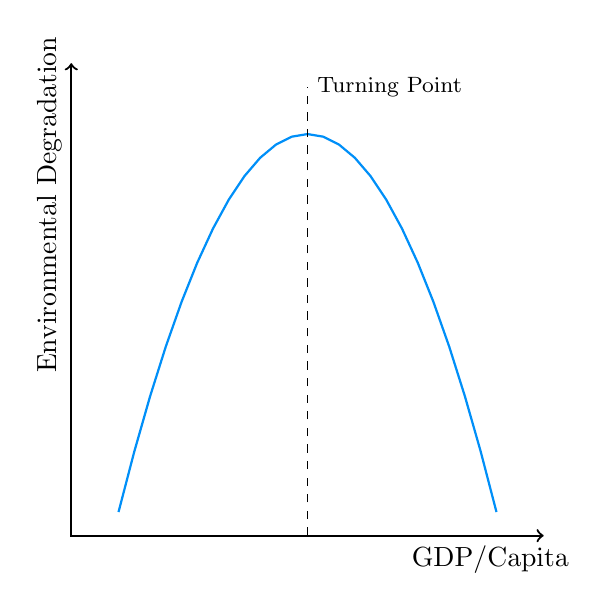
\begin{tikzpicture}[scale = 0.6]
\draw[thick, <->] (0,10) -- (0,0) -- (10,0);
\draw[thick, color1]  [domain = 1:9] plot (\x, {8.5 - .5*(\x - 5)^2});
\node [below right] at (7,0) {GDP/Capita};
\node[rotate=90, above] at (0,7) {Environmental Degradation};
\draw[dashed] (5,0) -- (5,9.5) node[right]{\footnotesize Turning Point};
\end{tikzpicture}
\end{minipage}
\begin{minipage}{0.48\textwidth}
\centering 
\caption{Application of the  EKC}
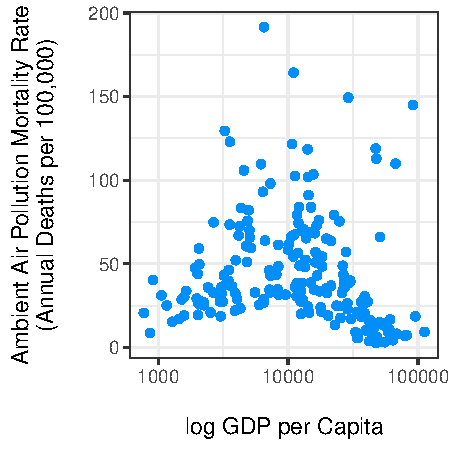
\includegraphics[width=0.9\textwidth]{figures/chapter2_figures/ekc.pdf}
\end{minipage}
Data from \cite{owidoutdoorairpollution} 
%https://ourworldindata.org/outdoor-air-pollution#outdoor-air-pollution-tends-to-rise-with-industrialization-before-falling
\end{figure}

Despite its quick adoption in the discipline and its continued use, the EKC has largely been discredited \citep{stern2004rise}. \cite{arrow1995economic} importantly note that the usual form of the EKC does not allow for any feedback between the environment and development, implicitly assuming that pollution and other forms of environmental degradation do not hinder economic development. 

The claim from the EKC that economic development itself will lead to improvements in environmental quality make dubious assumptions. The EKC correctly captures the tendency for rich nations to substitute dirty economic activities for relatively cleaner activities. Ultimately though, the world is finite, and some countries must house the high-pollution industries. This leads to what is known as the \emph{pollution haven hypothesis}. Stringent environmental regulation will raise the costs of firms in high-pollution industries, making firms in less-regulated economies relatively cheaper and more competitive. This means that some economies with relaxed environmental regulation might end up specializing in only high-pollution industries, becoming pollution havens. Thus, one consequence of environmental regulation may be that it shifts the burden of damaging economic activities elsewhere, usually to low- and middle-income countries. 

Contemporary empirical evidence on the pollution haven hypothesis leads to a few key conclusions: (1) environmental regulation does not have an economically significant effect overall trade flows, and (2) environmental regulation can have an economically significant effect on the trade flows of specific industries. A common technique for assessing differences in climate policies is considering differences in energy prices \citep[see for example][]{fowlie2022mitigating}. The idea is that carbon prices function in the short-run by raising the price of energy that a firm's technology limits them to use. Using differences in energy prices as a proxy, \cite{sato2015asymmetric} show that an increase in the energy price gap between trading countries only increases bilateral manufacturing trades by 0.2\%. Further these same energy price differences only explain 0.01\% of the variation in trade flows. \cite{aldy2015competitiveness} find a null result in a similar study looking at energy price differences between US states---the effect of energy price differences on total manufacturing imports between states was statistically insignificant, even with their over thirty years of panel data. However, they do find pronounced effects in certain, energy intensive sectors including steel, industrial chemicals, and cement. In their survey of the literature, \cite{dechezlepretre2020impacts} come to the conclusion that there is likely a pollution haven effect, but that it is confined to a select number of industries.

\textbf{Emissions Leakage}

If empirical evidence seems to suggest that climate policy only leads to significant competitive effects in a few industries, where is the problem? Unfortunately, even if the transfer of economic activity is small overall, the transfer of emissions can be quite large.

\emph{Emissions leakage} occurs when the implementation of stringent regulation (almost always meaning a carbon pricing scheme) on GHG emissions in one place leads to increased GHG emissions in another place with looser regulations. Emissions leakage is closely related to the pollution haven hypothesis, but differs in a few ways. First, emissions leakage refers exclusively to GHG emissions, not pollution in general. This distinction is important as most GHG emissions have a negligible effect on the areas downwind from their source of emissions, but ambient air pollutants do not. Thus, the consequences of increased GHGs from emissions leakage is global rather than local. Second, the pollution haven hypothesis is much more concerned with international trade flows and the changing composition of economies, whereas emissions leakage is concerned more with changing the distribution of emissions. That is, the pollution haven hypothesis focuses on the implications of displaced economic activity, and emissions leakage focuses on the implications of displaced emissions.

\begin{figure}
\caption{Competitive Emissions Leakage \label{leakage_ex}}
\centering
\singlespacing
\footnotesize
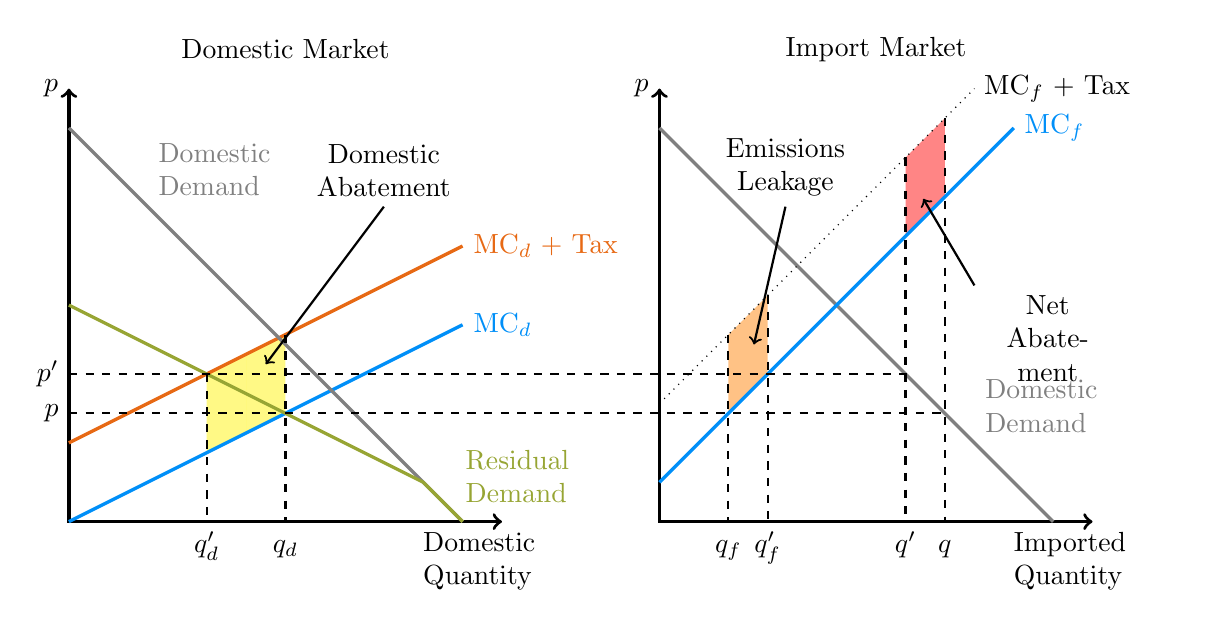
\begin{tikzpicture}[scale = 0.5]
	\draw[very thick, <->] (0, 11) node[left]{$p$} -- (0, 0) -- (11, 0) node[below, text width = 2cm]{Domestic Quantity};
	\draw[very thick, <->] (15, 11) node[left]{$p$} -- (15,0) -- (26, 0) node[below, text width = 2cm]{Imported Quantity};
	\fill[yellow!80!, opacity = 0.6] (3.5, 3.75) -- (3.5, 1.75) -- (4.5, 2.25) -- (4.5, 4.25) -- cycle;
	\fill[yellow!80!, opacity = 0.6] (4.5, 2.25) -- (5.5, 2.75) -- (5.5, 4.75) -- (4.5, 4.25) -- cycle;
	\fill[orange!80!, opacity = 0.6] (16.75, 4.75) -- (16.75, 2.75) -- (17.75, 3.75) -- (17.75, 5.75) -- cycle;
	%\fill[orange!80!, opacity = 0.6] (16.25, 4.25) -- (16.25, 2.25) -- (16.75, 2.75) -- (16.75, 4.75) -- cycle;
	\fill[red!80!, opacity = 0.6] (21.25, 9.25) -- (21.25, 7.25) -- (22.25, 8.25) -- (22.25, 10.25) -- cycle;
	%\fill[red!80!, opacity = 0.6] (20.75, 8.75) -- (20.75, 6.75) -- (21.25, 7.25) -- (21.25, 9.25) -- cycle;
	\draw[very thick, color1] (0,0) -- (10, 5) node[right]{MC$_d$};
	\draw[very thick, color3] (0,2) -- (10, 7) node[right]{MC$_d$ $+$ Tax};
	\draw[very thick, gray] (0, 10) -- (10,0) node[pos=.2, above right,text width = 1.5cm]{Domestic Demand}; 
	\draw[very thick, color2] (0,5.5) -- (9, 1) -- (10, 0) node[pos=.8, above right, text width = 1.5cm]{Residual Demand};
	%\draw[very thick, color2] (0, 6.5) -- (7,3) -- (10, 0);
	\draw[very thick, gray] (15, 10) -- (25, 0) node[pos=.8, above right,text width = 1.5cm]{Domestic Demand}; 
	\draw[very thick, color1] (15, 1) -- (24, 10) node[right, text width = 1.5cm]{MC$_f$};
	\draw[dashed, thick] (5.5, 4.75) -- (5.5, 0) node[below, yshift = -3pt]{$q_d$};
	\draw[dashed, thick] (3.5, 3.75) -- (3.5, 0) node[below]{$q_d'$};
	%\draw[dashed, thick] (4.5, 4.25) -- (4.5, 0) node[below]{$q_d''$};
	\draw[dashed, thick] (0, 3.75) node[left]{$p'$} -- (21.25, 3.75);
	\draw[dashed, thick] (0, 2.75) node[left]{$p$} -- (22.25, 2.75);
	%\draw[dashed, thick] (0,4.25) node[left]{$p''$} -- (20.75, 4.25);
	\draw[dashed, thick] (16.75,4.75) -- (16.75, 0) node[below, yshift = -3pt]{$q_f$};
	\draw[dashed, thick] (17.75, 5.75) -- (17.75, 0) node[below]{$q_f'$};
	%\draw[dashed, thick] (16.25, 4.25) -- (16.25, 0) node[below]{$q_f''$};
	\draw[dashed, thick] (22.25, 10.25) -- (22.25, 0) node[below, yshift = -3pt]{$q$};
	\draw[dashed, thick] (21.25, 9.25) -- (21.25, 0) node[below]{$q'$};
	%\draw[dashed, thick] (20.75, 8.75) -- (20.75, 0) node[below]{$q''$};
	\draw[dotted] (15, 3) -- (23, 11) node[right]{MC$_f$ $+$ Tax};
	\draw[thick, <-] (5, 4) -- (8, 8) node[above, text width = 2cm, align=center]{Domestic Abatement};
	\draw[thick, <-] (17.4, 4.5) -- (18.2, 8) node[above, text width = 2cm, align=center]{Emissions Leakage}; 
		\draw[thick, <-] (21.7, 8.2) -- (23, 6) node[below right, text width = 1.6cm, align=center]{Net Abatement};
		\node at (5.5, 12) {Domestic Market};
		\node at (20.5, 12) {Import Market}; 
\end{tikzpicture}
\end{figure}

Figure \ref{leakage_ex} displays how competitive effects can drive emissions leakage in an example market. In the left panel of figure \ref{leakage_ex} is the domestic market for an emissions creating good. In the right panel of figure \ref{leakage_ex} is the import market for the same good. Domestic producers do not face the full domestic demand curve, as foreign producers will also be willing to supply the domestic market. Instead, domestic producers face the residual demand curve, the difference between the domestic quantity demanded and the import supply at each price. Domestic firms will produce where their marginal cost curve MC$_d$ intersects residual demand. This price then caries into the import market, and foreign firms will produce where the domestic market price intersects their marginal cost curve MC$_f$. Absent any carbon pricing scheme, domestic firms produce $q_d$, foreign firms import $q_f$, and the total market quantity is $q$. 

Now suppose that domestic policymakers implement a carbon pricing scheme. For ease, assume that this takes the form of a per ton emissions tax and that marginal emissions and marginal damages from emissions are both constant. The carbon pricing scheme is unilateral, meaning that it applies to all domestic producers, but not any foreign producers. The constant marginal emissions rate and per unit carbon tax imply that domestic firms pay a constant per unit tax on their output, creating a parallel shift up in from MC$_d$ to MC$_d$ $+$ Tax. Again, firms produce where the marginal cost they face equals residual demand. This causes the domestic price of the good to rise to $p'$ and the domestic production of the good to fall to $q_d'$. The yellow region of left panel in figure \ref{leakage_ex} represents a monetary measure of domestic abatement. If the tax on emissions is set to the social cost of a ton of emissions, then this area is the monetary value of all domestic emissions abatement $\tau E_d$, where $E_d$ is the sum of domestic emissions in the market. Like we should expect, the carbon pricing scheme induces domestic reductions in GHG emissions.

Unfortunately, this is not the case in the import market. Unlike firms in the domestic market, foreign firms do not face this same emissions price. Higher prices in the domestic market without the counteracting increase in costs induce foreign firms to expand their production from $q_f$ to $q_f'$. Analogous to the yellow area, the orange area in the right panel of figure \ref{leakage_ex} represents the social cost of the additional emissions in the import market. This is emissions leakage: an increase foreign emissions as a result of unilateral carbon pricing. Still, unilateral carbon pricing manages to reduce total emissions despite the leakage. Total quantity in the domestic market falls from $q$ to $q'$, with the area of the red region representing the social value of the net abatement. We see that when we take leakage into account, the emissions reductions are much more modest than what they appeared to from domestic production alone. 

There are a certain class of goods that are particularly susceptible to emissions leakage known as \emph{emissions-intensive and trade-exposed} (EITE) goods. A good is emissions intensive if its production creates a lot of emissions per unit (tons of CO$_2$e/\$). We measure the trade exposure of a good with the ratio of the volume traded domestically (value of imports $+$ value of exports) to the total volume of good that passes through the domestic economy (value of domestic production $+$ value of imports). \cite{fowlie2022mitigating} and \cite{fowlie2016measuring} show that it is not enough to be only emissions intensive or only trade exposed to have a high risk of leakage. Both conditions are necessary to have a substantial risk of emissions leakage. EITE goods include cement, steel, and many industrial chemicals.

The bad news of emissions leakage does not end there. There are many ways that emissions leakage can occur. Using the language of \cite{cosbey2020developing}, we have so far discussed the \emph{competitiveness channel}, where emissions increase outside of the regulated jurisdiction as unregulated producers become more competitive. Another important form of leakage occurs through the \emph{energy market channel}. If the US implemented a stringent tax on GHG from cars, we can expect that the domestic demand of gasoline will fall dramatically as US commuters opt for modes of transportation other than gas-fueled vehicles (e.g., electric vehicles, bikes, public transit). The US is large enough though that this will cause prices to fall in global energy markets, and when fuels like petroleum-based fuels become cheaper, more firms will begin using petroleum-based fuels and creating more emissions elsewhere. These general equilibrium effects that move in and around global energy markets are difficult to address without globally coordinated efforts to ditch fossil fuels. These two channels are thought to be the primary drivers of leakage \citep{branger2014climate}

There are also a few ways where we might see negative emissions leakage. That is, situations where ambitious steps towards abatement in one location spillover into abatement somewhere else. The \emph{income channel} provides another opportunity for negative leakage. If a carbon tax makes people poorer in less-regulated jurisdictions, then this could decrease foreign consumption and production of emissions intensive goods and lower emissions. Of course, this is not a favorable way to reduce emissions. The income channel could operate in the opposite direction as well, raising emissions in places where incomes increase as a result of the incomplete regulation. The more likely form of negative leakage occurs through the \emph{technology channel}. Carbon pricing schemes reduce emissions not just by internalizing the externality, but by providing incentives for the creation of new, cleaner technologies. Producers facing emissions pricing certainly have an incentive to adopt cleaner technologies, but producers outside of the regulated region do not have this same carrot and stick. If these new technologies happen to be more cost-effective than existing technologies, then it is possible that producers would adopt these cleaner technologies and reduce emissions this way. The prospect of negative emissions leakage is overly optimistic as a whole, and empirical evidence to date suggests that negative leakage is negligible compared to the other channels of leakage \citep{winchester2013numerical}.

\textbf{Charges, Rebates, and Permits---Oh My!}

An important approach to completing emissions regulations is through border carbon adjustments. Border carbon adjustments (BCAs) are policies that manipulate the price of goods as they move between jurisdictions with different emissions prices, usually between one place with a carbon price and another without a carbon price. That is, these policies adjust the price of goods based on their carbon emissions (or carbon equivalent emissions) at the border. They come in two major varieties: import taxes (charges) and export (output) rebates

\emph{Import taxes} or \emph{import charges} attempt to complete the regulation of domestic markets by subjecting foreign imports to carbon taxes similar to the carbon taxes domestic producers pay. Import charges are the more relevant of the two major varieties of BCAs, and often we use the term BCA when we just mean import charges. This is largely because we import more EITE goods than we export. 

Figure \ref{import_charge} displays how an emissions charge on imports can reduce leakage. Like in figure \ref{leakage_ex}, suppose that domestic firms pay a constant tax for each ton of their GHG emissions. For simplicity, assume that all producers, domestic and foreign, have a constant, identical emissions intensity. With the unilateral emissions tax and without an import charge, there is substantial domestic abatement---represented by the orange and yellow regions in the domestic market---and there is substantial leakage---represented by the red region in the import market. The total emissions reductions are represented by the violet region in the import market. 

Consider now when policymakers impose an import charge analogous to the domestic emissions tax. Now foreign producers face MC$_f$ $+$ Tax, a parallel shift of their previous marginal cost curve. With the marginal cost curve shifting back in the import market, the difference between the domestic quantity demanded and the quantity of imports supplied increases at every price level. As a result, residual demand in the domestic market shifts up. Setting this new residual demand curve RD$''$ equal to the marginal cost MC$_d$ $+$ Tax, increases the domestic quantity from $q_d'$ to $q_d''$. This means that the value of domestic abatement decreases from the sum of areas of the orange and yellow regions in domestic market to just the area of the yellow region. Although there is modest increase in domestic emissions due to the import charge, there is larger reduction in foreign emissions. The import charge moves foreign production from $q_f'$ to $q_f''$. Previous to the imposition of the import charge, the unilateral emissions tax increased the costs of foreign emissions by the area of the red region in the import market. With the imposition of the import charge though, we see that foreign emissions are actually less than they were in the baseline (no domestic emissions tax and no import charge). The social value of this foreign abatement is give by the area of the region in blue. The total quantity of the good in the domestic market decreases from $q_d'$ to $q_d''$. The additional social value of emissions abatement due to the import charge is given by the area of the green region in the import market.

Import charges bring with them a host of technical challenges that for the most part tie back to one central question: how do we assess the emissions of imported goods? 

\begin{figure}
\caption{Leakage with an Import Charge \label{import_charge}}
\centering
\singlespacing
\footnotesize
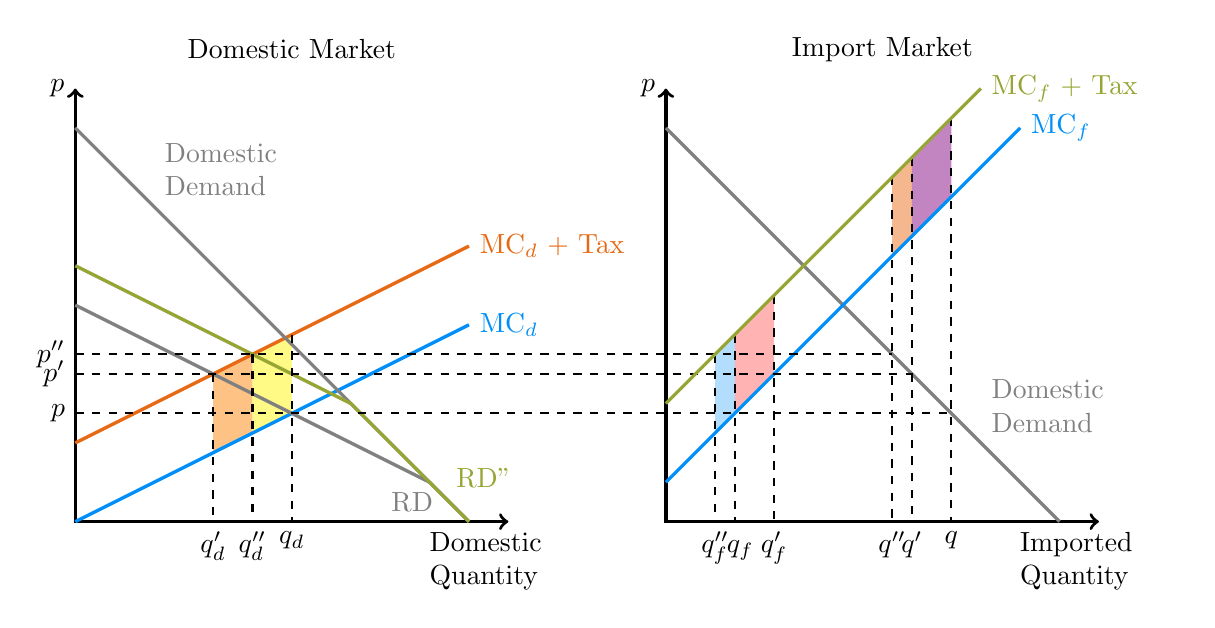
\begin{tikzpicture}[scale = 0.5]
	\draw[very thick, <->] (0, 11) node[left]{$p$} -- (0, 0) -- (11, 0) node[below, text width = 2cm]{Domestic Quantity};
	\draw[very thick, <->] (15, 11) node[left]{$p$} -- (15,0) -- (26, 0) node[below, text width = 2cm]{Imported Quantity};
	\fill[orange!80!, opacity = 0.6] (3.5, 3.75) -- (3.5, 1.75) -- (4.5, 2.25) -- (4.5, 4.25) -- cycle;
	\fill[yellow!80!, opacity = 0.6] (4.5, 2.25) -- (5.5, 2.75) -- (5.5, 4.75) -- (4.5, 4.25) -- cycle;
	\fill[red!50!, opacity = 0.6] (16.75, 4.75) -- (16.75, 2.75) -- (17.75, 3.75) -- (17.75, 5.75) -- cycle;
	\fill[color1!50!, opacity = 0.6] (16.25, 4.25) -- (16.25, 2.25) -- (16.75, 2.75) -- (16.75, 4.75) -- cycle;
	\fill[violet!80!, opacity = 0.6] (21.25, 9.25) -- (21.25, 7.25) -- (22.25, 8.25) -- (22.25, 10.25) -- cycle;
	\fill[color3!80!, opacity = 0.6] (20.75, 8.75) -- (20.75, 6.75) -- (21.25, 7.25) -- (21.25, 9.25) -- cycle;
	\draw[very thick, color1] (0,0) -- (10, 5) node[right]{MC$_d$};
	\draw[very thick, color3] (0,2) -- (10, 7) node[right]{MC$_d$ $+$ Tax};
	\draw[very thick, gray] (0, 10) -- (10,0) node[pos=.2, above right,text width = 1.5cm]{Domestic Demand}; 
	\draw[very thick, gray] (0,5.5) -- (9, 1) -- (10, 0) node[pos=.5, left, xshift = -2pt]{RD};
	\draw[very thick, color2] (0, 6.5) -- (7,3) -- (10, 0) node[pos=.8, above right, text width = 1.5cm]{RD''};
	\draw[very thick, gray] (15, 10) -- (25, 0) node[pos=.8, above right,text width = 1.5cm]{Domestic Demand}; 
	\draw[very thick, color1] (15, 1) -- (24, 10) node[right, text width = 1.5cm]{MC$_f$};
	\draw[dashed, thick] (5.5, 4.75) -- (5.5, 0) node[below]{$q_d$};
	\draw[dashed, thick] (3.5, 3.75) -- (3.5, 0) node[below]{$q_d'$};
	\draw[dashed, thick] (4.5, 4.25) -- (4.5, 0) node[below]{$q_d''$};
	\draw[dashed, thick] (0, 3.75) node[left]{$p'$} -- (21.25, 3.75);
	\draw[dashed, thick] (0, 2.75) node[left]{$p$} -- (22.25, 2.75);
	\draw[dashed, thick] (0,4.25) node[left]{$p''$} -- (20.75, 4.25);
	\draw[dashed, thick] (16.75,4.75) -- (16.75, 0) node[below, yshift = -3pt, xshift = 2pt]{$q_f$};
	\draw[dashed, thick] (17.75, 5.75) -- (17.75, 0) node[below]{$q_f'$};
	\draw[dashed, thick] (16.25, 4.25) -- (16.25, 0) node[below]{$q_f''$};
	\draw[dashed, thick] (22.25, 10.25) -- (22.25, 0) node[below]{$q$};
	\draw[dashed, thick] (21.25, 9.25) -- (21.25, 0) node[below]{$q'$};
	\draw[dashed, thick] (20.75, 8.75) -- (20.75, 0) node[below]{$q''$};
	\draw[color2, very thick] (15, 3) -- (23, 11) node[right]{MC$_f$ $+$ Tax};
	%\draw[thick, <-] (5, 4) -- (8, 8) node[above, text width = 2cm, align=center]{Domestic Abatement};
	%\draw[thick, <-] (16.7, 4.5) -- (18, 8) node[above, text width = 2cm, align=center]{Emissions Leakage}; 
		%\draw[thick, <-] (21.6, 8) -- (23, 6) node[below right, text width = 1.6cm, align=center]{Net  Abatement};
	\node at (5.5, 12) {Domestic Market};
		\node at (20.5, 12) {Import Market}; 
\end{tikzpicture}
\smallskip
Adapted from \cite{fowlie2016measuring}.
\end{figure}

Before we determine how to assess the emissions of imported goods, it is useful to know how we assess the emissions of domestically produced goods. The GHG Protocol, the internationally recognized leader in GHG emissions accounting standards, sets out three emissions scopes. Figure \ref{scopes} summarizes these three different methods to account for an organization’s emissions \citep{ghg_protocol_2011}. Scope 1 looks at just an organization’s direct emissions, like the GHGs that the organization emits on site. Scope 2 includes all these direct emissions from Scope 1, but also includes indirect emissions associated with energy inputs. For instance, a database center might have relatively low Scope 1 emissions, but if all electric power needed for the database center comes from a coal-fueled plant, Scope 2 emissions would be high. Scope 3 takes this a step further to look at the lifecycle emissions associated with an organization. This includes all the emissions captured by Scope 2, and includes emissions embodied in non-energy inputs and downstream emissions from distribution, processing, use, and disposal of its output. Any domestic emissions pricing program first needs to determine what emissions it will use to assess emissions to firms. It is best practice to assess foreign emissions with the same scope as domestic emissions, and likely violates international trade law to assess emissions using a higher scope for foreign producers \citep{cosbey2020developing}.

\begin{figure}
	\caption{Greenhouse Gas Emissions Scopes \citep{ghg_protocol_2011}\label{scopes}}
	\centering
	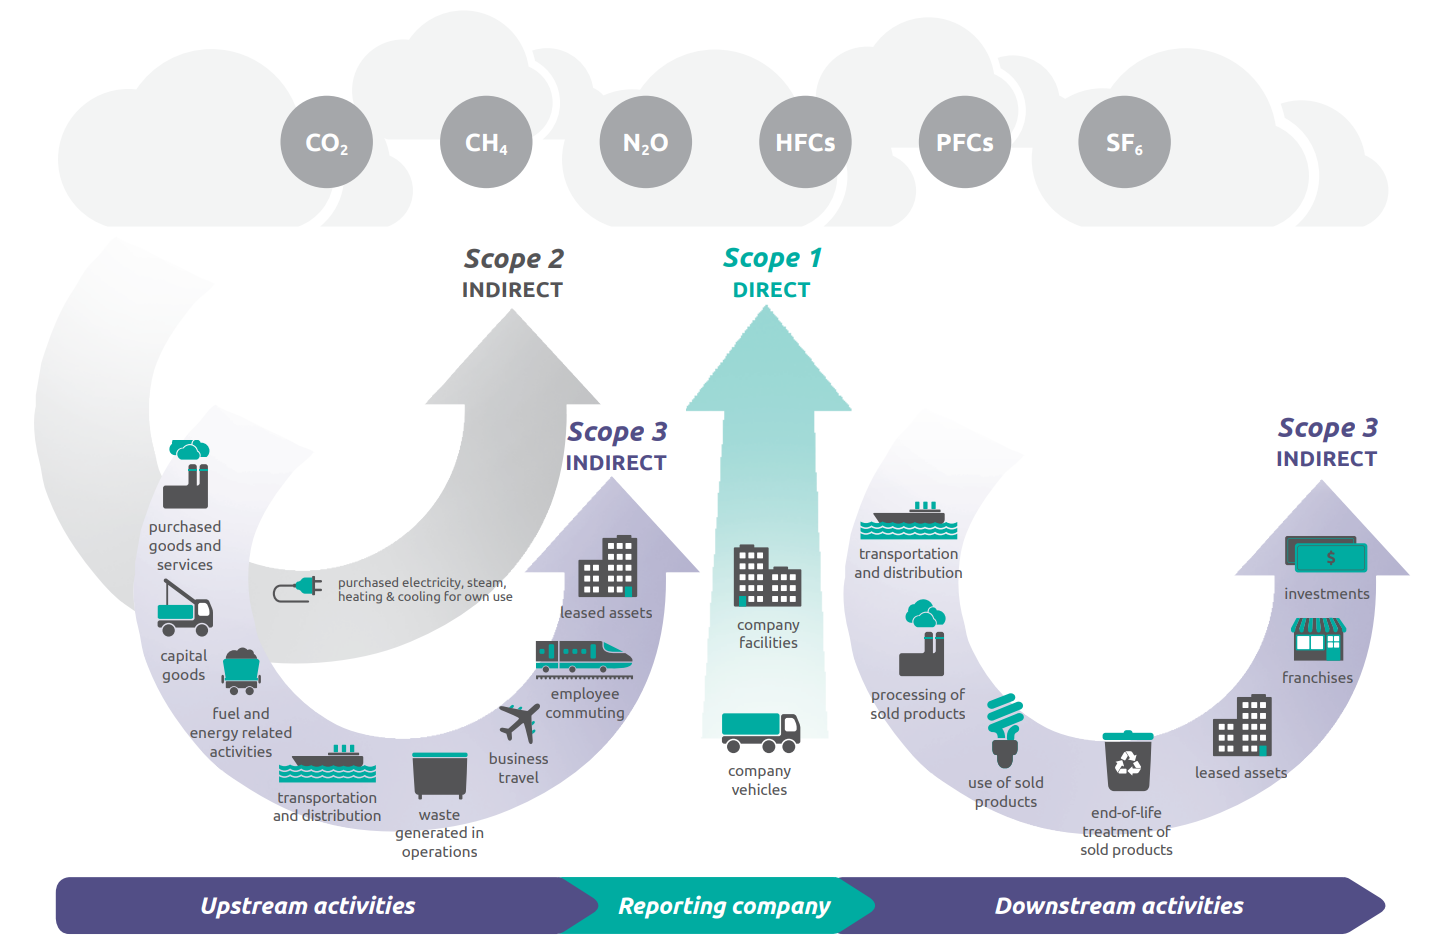
\includegraphics[width=0.8\textwidth]{figures/chapter2_figures/ghg_scope.png}
\end{figure}

In their most complete form, border carbon adjustments cover all goods that cross the border, not just imports. Just like highly-regulated domestic production will likely have a cost disadvantage in the domestic market, highly-regulated exports will likely have a cost disadvantage in foreign markets. To prevent jurisdictions with ambitious climate policy from losing their exports requires some way to adjust the price of exports. This is the purpose of an \emph{export rebate}, often just called an \emph{output rebate}.

An output rebate pays back a flat rate to domestic producers for every unit they export. While carbon taxes on imports try to even the playing field between highly regulated and less regulated producers in domestic markets, output rebates try to even the playing field between highly regulated and less regulated producers on foreign markets. For instance, if US fertilizer manufacturers export much of their product, imposing a domestic carbon tax raises these manufacturers’ costs relative to their competitors overseas. This cost differential may allow foreign fertilizer manufacturers to retake some of the (foreign) market share from US fertilizer manufacturers. This increased foreign production will lead to greater GHG emissions associated with the foreign fertilizer market, a problem that may be exacerbated if foreign manufacturers were already more emissions intensive than US manufacturers.

Output rebates lack the same intuitive appeal that an emissions tax on imports have. After all, why should we tax manufacturers only to pay them back? Why not just tax manufacturers the difference between the original emissions tax and the output rebate? The first reason is a matter of accounting. Output rebates only apply to exports, so reducing the tax on all goods would not differentiate between the goods that should and should not receive a subsidy to avoid leakage. The second reason is a matter of incentives. Output rebates are not refunds on emissions taxes, as the government pays these out for every unit of output rather than for every ton of GHG emissions. In a world where goods had a fixed emissions intensity, this difference would not matter. Thankfully though, there are ways to reduce emissions without reducing output (e.g., switching to cleaner inputs or installing smokestack scrubbers). Thus, an output rebate will maintain the same abatement incentive on exports, while also allowing domestic producers to maintain their ability to compete in foreign markets. The low volume of US manufacturing exports relative to imports means that these are not typically the primary concern in anti-leakage policy.

%\begin{figure}
%\caption{Leakage with an Emissions Tax on Imports}
%\centering
%\singlespacing
%\footnotesize
%\begin{tikzpicture}[scale = 0.5]
%	\draw[very thick, <->] (0, 11) node[left]{$p$} -- (0, 0) -- (11, 0) node[below, text width = 2cm]{Domestic Quantity};
%	\draw[very thick, <->] (15, 11) node[left]{$p$} -- (15,0) -- (26, 0) node[below, text width = 2cm]{Imported Quantity};
%	\fill[orange!80!, opacity = 0.6] (3.5, 3.75) -- (3.5, 1.75) -- (4.5, 2.25) -- (4.5, 4.25) -- cycle;
%	\fill[yellow!80!, opacity = 0.6] (4.5, 2.25) -- (5.5, 2.75) -- (5.5, 4.75) -- (4.5, 4.25) -- cycle;
%	\fill[orange!80!, opacity = 0.6] (16.75, 4.75) -- (16.75, 2.75) -- (17.75, 3.75) -- (17.75, 5.75) -- cycle;
%	\fill[yellow!80!, opacity = 0.6] (16.25, 4.25) -- (16.25, 2.25) -- (16.75, 2.75) -- (16.75, 4.75) -- cycle;
%	\fill[orange!80!, opacity = 0.6] (21.25, 9.25) -- (21.25, 7.25) -- (22.25, 8.25) -- (22.25, 10.25) -- cycle;
%	\fill[yellow!80!, opacity = 0.6] (20.75, 8.75) -- (20.75, 6.75) -- (21.25, 7.25) -- (21.25, 9.25) -- cycle;
%	\draw[very thick, color1] (0,0) -- (10, 5) node[right]{MC$_d$};
%	\draw[very thick, color3] (0,2) -- (10, 7) node[right]{MC$_d$ $+$ Tax};
%	\draw[very thick, gray] (0, 10) -- (10,0) node[pos=.2, above right,text width = 1.5cm]{Domestic Demand}; 
%	\draw[very thick, color2] (0,5.5) -- (9, 1) -- (10, 0) node[pos=.8, above right, text width = 1.5cm]{Residual Demand};
%	\draw[very thick, color2] (0, 6.5) -- (7,3) -- (10, 0);
%	\draw[very thick, gray] (15, 10) -- (25, 0) node[pos=.8, above right,text width = 1.5cm]{Domestic Demand}; 
%	\draw[very thick, color1] (15, 1) -- (24, 10) node[right, text width = 1.5cm]{MC$_f$};
%	\draw[dashed, thick] (5.5, 4.75) -- (5.5, 0) node[below]{$q_d$};
%	\draw[dashed, thick] (3.5, 3.75) -- (3.5, 0) node[below]{$q_d'$};
%	\draw[dashed, thick] (4.5, 4.25) -- (4.5, 0) node[below]{$q_d''$};
%	\draw[dashed, thick] (0, 3.75) node[left]{$p'$} -- (21.25, 3.75);
%	\draw[dashed, thick] (0, 2.75) node[left]{$p$} -- (22.25, 2.75);
%	\draw[dashed, thick] (0,4.25) node[left]{$p''$} -- (20.75, 4.25);
%	\draw[dashed, thick] (16.75,4.75) -- (16.75, 0) node[below, yshift = -3pt, xshift = 2pt]{$q_f$};
%	\draw[dashed, thick] (17.75, 5.75) -- (17.75, 0) node[below]{$q_f'$};
%	\draw[dashed, thick] (16.25, 4.25) -- (16.25, 0) node[below]{$q_f''$};
%	\draw[dashed, thick] (22.25, 10.25) -- (22.25, 0) node[below]{$q$};
%	\draw[dashed, thick] (21.25, 9.25) -- (21.25, 0) node[below]{$q'$};
%	\draw[dashed, thick] (20.75, 8.75) -- (20.75, 0) node[below]{$q''$};
%	\draw[color2, very thick] (15, 3) -- (23, 11) node[right]{MC$_f$ $+$ Tax};
%	%\draw[thick, <-] (5, 4) -- (8, 8) node[above, text width = 2cm, align=center]{Domestic Abatement};
%	%\draw[thick, <-] (16.7, 4.5) -- (18, 8) node[above, text width = 2cm, align=center]{Emissions Leakage}; 
% 	%\draw[thick, <-] (21.6, 8) -- (23, 6) node[below right, text width = 1.6cm, align=center]{Net Abatement};
% 	\node at (5.5, 12) {Domestic Market};
% 	\node at (20.5, 12) {Foreign Imports}; 
%\end{tikzpicture}
%\end{figure}

%%%%%%%%%%%
\newpage
\section{Leakage \& BCAs in the California Power Industry}

\subsection{A Perfectly Competitive Model of Leakage}

Here we consider a perfectly competitive model of emissions leakage in the Western Interconnection based largely off of \cite{fowlie2021border}. We begin constructing a model where there is no emissions pricing scheme and then impose an emissions tax. Alongside the emissions tax, we consider different possible border carbon adjustments with the potential to reduce leakage. 

This is not a model of residential electric power markets. Residential electric power prices involve complicated tier systems, connection charges, and many additional fees that distort the true price. In addition to discouraging electrification \citep[see][]{borenstein2021designing}, these structures make simulating these markets impractical in this analysis. Instead, we model the wholesale day-ahead electricity market. 

The Federal Energy Regulatory Commission's \emph{Energy Primer} \citep{ferc2020} describes how power grid operators and power plants decide what generation will take place. Power grid operators have the goal of ensuring reliable power supply at the least cost. This process plays out in two stages. In the first stage, operators prepare for forecasted demand by committing generators a day before. This is the day-ahead market, where power plants sell their generation in anticipation for the next day. In the second stage, operators make adjustments in real-time by calling on additional generators to either turn on or off through a process called Automatic Generation Control. Grid operators determine whether or not to increase generation by measuring the frequency (cycles/second) of the AC power lines. In the US, operators aim for a frequency of 60 Hz, so a frequency above or below 60 Hz means that the too much or too little generation respectively. 

The structure of these day-ahead markets varies considerably across the country. One important factor in identifying the structure of these markets is the existence of a Regional Transmission Operator (RTO) or an Independent System Operator (ISO). RTOs and ISOs are essentially two different names for the same entity.\footnote{\cite{rff_podcast1} says ``At one point, FERC---the Federal Energy Regulatory Commission---made a distinction between these entities. It's a distinction without a difference at this point."} These entities are non-profit organizations that have the primary responsibility of operating markets for electric power
across many generators (the power plants, i.e. the sellers of electricity) and load-serving organizations (utilities, large industrial users, i.e. the buyers of electricity). \cite{ferc2020} gives an excellent description of how these day-ahead markets operate under an RTO or ISO.
\begin{quote}
In day-ahead markets, the schedules for supply and usage of energy are compiled hours ahead of the beginning of the operating day. The RTO/ISO then runs a computerized market model that matches buyers and sellers throughout the market footprint for each hour throughout the day. The model then evaluates the bids and offers of the participants, based on the power flows needed to move the electricity throughout the grid from generators to consumers. Additionally, the model must account for changing system capabilities that occur, based on weather and equipment outages, plus the rules and procedures that are used to ensure system reliability. The market rules dictate that generators submit supply offers and that loads submit demand bids to the RTO/ISO by a deadline that is typically in the morning of the day-ahead scheduling. Typically, 95 percent of all load is scheduled in the day-ahead market and the rest is scheduled in real-time.
\end{quote}
This means that the wholesale day-ahead market has many of the characteristic features of a competitive market. The good bought and sold is homogeneous, and buyers have little ability to differentiate between  sellers. There are thousands of power plants selling power in any RTO/ISO and dozens of utilities and industrial costumers buying it. Moreover RTOs/ISOs dispatch additional generating units based on their marginal costs, which is suggestive that supply in the market is allocated competitively. Given this market structure, it seems most sensible to model this market as perfectly competitive. 

% \subsubsection*{The General Model}

% Consider a model of the Western Interconnection. Denote the set of all power plants in the interconnection as $N$ and the subset of power plants located in California with $N_\text{Cal}$. The set of regions $R$ in the interconnection, each with its own market for electric power and its own generation. For now, assume these markets behave competitively. Further, assume that plants in each regional market face linear inverse demand curves with the form
% \begin{equation}
% 	p_r = \alpha_r - \beta_r Q_r
% \end{equation}
% where $p_r$ is the price in region $r$ (\$/MWh), $Q_r$ is the total quantity of power demanded in region $r$ (MWh), and $\alpha_r$ and $\beta_r$ are regional constants. 

% Each power plant decides how much power to generate for each regional market. Let $q_{ir}$ denote the power in MWh that plant $i$ generates to sell in regional market $r$. Any plant can generate power for any other region, regardless of what region the plant is located in. 

% We can group all power plants into one of two groups: fossil fuel plants and non-fossil fuel plants. Fossil fuel plants each have a plant specific marginal cost that depends on some of the physical features of its generators and the cost of the fuel it uses (natural gas, coal, or occasionally, oil). Fossil fuel plants choose how much power to generate based on their marginal costs and the prices in each market. 

% Non-fossil fuel plants do not have such clear marginal costs. For instance, a windfarm does not decide how much power to generate based on its marginal cost, but is constrained the generate whatever the environment allows it to. We make the assumption that the total generation for any individual non-fossil fuel plant is fixed, and they have not marginal cost. Note that although the total generation of these plants is fixed, the allocation of their generation is not. These plants can still choose how much of their power to sell in each region. 

% While we might usually endow individual firms with behaviors (objective functions) and try to solve analytically for their aggregate outcome, here we endow the entire interconnection with a behavior instead. Standard economic theory says that the perfectly competitive outcome uniquely maximizes total surplus. Then to simulate this market, we need to find what generation and allocation from each plant maximizes the sum of the areas under the demand curve in each regional market minus any marginal costs, including costs from congestion, carbon taxes, and BCAs. The area under the demand curve in region $r$ is a trapezoid with area
% $$\frac12 \left[\alpha + \left( \alpha_r - \beta_r Q_r^*\right)\right] Q_r^* = \frac12 \left( 2\alpha_r - \beta_r \sum_{i \in N} q_{ir} \right) \sum_{i \in N} q_{ir}$$
% where $Q_r^*$ is the equilibrium quantity regional market $r$. This leads the the optimization problem:
% \begin{align*}
% \max_{\{q_{ir}\}} \hspace{2em}\left\{\sum_{r\in R} \left[ \frac12 \left( 2\alpha_r - \beta_r \sum_{i \in N} q_{ir} \right) \sum_{i \in N} q_{ir}\right] - \left(\sum_{(i, r) \in N \times R} c_i q_{ir}\right) - \tau \left(\sum_{(i, r) \in N \times R} \widetilde{e_{ir}} q_{ir}\right)\right\}
% \end{align*}
% where $\tau$ is the emissions tax (\$/ton of CO$_2$e) and $\widetilde{e_{ir}}$ is the assessed emissions intensity. This assessed emissions intensity is the emissions intensity that policies tax at. As we lay out next, each policy functions by changing what the assessed emissions intensity is for each plant-region pair. The first term in the objective function is the sum of the areas under the demand curves. The second term is the total total marginal operating cost, and the third term is the total emissions cost. The optimization problem is subject to the following constraints:
% \begin{gather*}
% 	q_{ir} \geq 0, ~\text{for all plants} ~i~ \text{and regions} ~r\\
% 	\sum_{r \in R} q_{ir} \leq q_i^\text{max}, ~\text{for all fossil fuel plants} ~i\\
% 	\sum_{r \in R} q_{ir} = \overline{q}_i, ~\text{for all non-fossil fuel plants} ~i\\
% 	\left(\sum_{i \in N_{r}} q_{is}\right)  + \left(\sum_{i \in N_s} q_{ir}\right) \leq T_{(r,s)}, ~\text{for all}~(r,s) \in N\times N ~\text{such that}~ r \neq s
% \end{gather*}
% The first constraint guarantees that plants do not try to generate negative power for a region---they can only generate power at their own plant. The second constraint restricts fossil fuel power plants to their maximum generation (i.e., their nameplate capacity). Non-fossil fuel power plants do not have marginal costs, so the third constraint set the total generation of a non-fossil fuel plant to an exogenous quantity. The final constraint is the transmission constraint. This says that for any two distinct regions $r$ and $s$, the sum of their exports to the other region cannot exceed the maximum transmission load of the lines between them $T_{(r,s)}$. If there were no transmission constraints, nearly total leakage would be  practically guaranteed as trade is completely exposed.

% \begin{table}
% \caption{Notation Summary}
% \centering
% \begin{tabular}{c p{10cm}}
% \hline\hline
% Notation & Description \\
% \hline
% 	$N$ & Set of power plants\\
% 	$R$ & Set of regions\\
% 	$i$ & Subscript denoting an arbitrary power plant, $\i \in N$\\
% 	$r$ & Subscript denoting an arbitrary region, $r \in R$\\
% 	$q_{ir}$ & Plant $i$'s generation to sell in region $r$ (MWh)\\
% 	$q_i^\text{max}$ & Fossil fuel plant $i$'s exogenously determined maximum generation (MWh)\\
% 	$\overline{q}_i$ & Non-fossil fuel plant $i$'s exogenously determined total generation (MWh)\\
% 	$p_r$ & Market price in region $r$\\
% 	$Q_r$ & Generation to sell in region $r$, $Q_r = \sum_{i=1}^N q_{ir}$\\
% 	$e_i$ & Actual emissions intensity of plant $i$ (tons CO$_2$e)\\
% 	$\widetilde{e_{ir}}$ & Assessed emission intensity; emissions intensity for tax purposes of plant $i$ selling in region $r$\\
% 	$d$ & Default emissions intensity\\
% \hline	\hline
% \end{tabular}
% \end{table}

% \subsubsection*{Scenario A: No Regulation}

% Under no regulation, policymakers do not assess emissions to any power plant. That is, $\widetilde{e_{ir}} = 0$.

% \subsubsection*{Scenario B: Complete Regulation}

% Under complete regulation, all plants pay a tax based on their actual emissions intensity in each market. Then set $\widetilde{e_{ir}} = e_i$ for each $i \in N$ and $r \in R$. 

% \subsubsection*{Scenario C: California Carbon Tax, No BCA}

% In this scenario, California implements a domestic carbon tax without a BCA. This means that all plants in California pay a tax based on their actual emissions intensity, but no other plants pay an emissions tax. Then set
% \[
% \widetilde{e_{ir}} = \begin{cases}
% 	~~e_i & \text{if}~~i\in N_\text{Cal}\\
% 	~~0 & \text{if}~~i\not\in N_\text{Cal}.
% \end{cases}
% \]

% \subsubsection*{Scenario D: California Carbon Tax, Uniform BCA}

% Once again, all plants in California face a domestic carbon tax and pay based on their actual emissions intensity. With the uniform BCA though, all plants outside of California pay an emissions tax on the power they export to California. Regardless of their actual emissions intensity, all plants exporting power to California face a default emissions intensity, $d$. In this scenario,
% \[
% \widetilde{e_{ir}} = \begin{cases}
% 	~~e_i & \text{if}~~i\in N_\text{Cal}\\
% 	~~d & \text{if}~~i\not\in N_\text{Cal} ~~\text{and}~~ r = \text{California}\\
% 	~~0 & \text{if}~~i\not\in N_\text{Cal} ~~\text{and}~~ r \neq \text{California}.
% \end{cases}
% \]

% \subsubsection*{Scenario E: California Carbon Tax, Differentiated BCA}

% Lastly, this scenario models a differentiated BCA. The assessed emissions intensities of all California plants is again their actual emissions intensity. Plants outside of California can choose to either pay their actual emissions intensity the default emissions rate, $d$. Assume that plants always choose the lower emissions intensity, so that clean plant with $e_i < d$ will choose to pay using their actual emissions rate and dirty plants with $e_i \geq d$ will choose to pay using the default emissions intensity. This means,
% \[
% \widetilde{e_{ir}} = \begin{cases}
% 	~~e_i & \text{if}~~i\in N_\text{Cal}\\
% 	~~e_i & \text{if}~~i\not\in N_\text{Cal} ~~\text{and}~~ r = \text{California} ~~\text{and}~~ e_i < d \\
% 	~~d & \text{if}~~i\not\in N_\text{Cal} ~~\text{and}~~ r = \text{California} ~~\text{and}~~ e_i \geq d \\
% 	~~0 & \text{if}~~i\not\in N_\text{Cal} ~~\text{and}~~ r \neq \text{California}.
% \end{cases}
% \]


% \subsection{Data}

% Estimating the simulation requires data on all individual power plants, regional electric power markets, and transmission across the entire Western Interconnection. 

% Regional market data comes from US Energy Information Administration's (EIA) Hourly Electric Grid Monitor from 2019. I pull daily generation data by region and by fuel type for the Western Electric Coordinating Council, which governs the Western Interconnection. This aggregates the Western Interconnection into three regions: California, the Northwest, and the Southwest. Additionally, I pull price data from spot markets in each of these regions from the Inter-Continental Exchange (ICE) for the  247 days it is available in 2019. 

% Power plant data comes from the EPA's 2019 Emissions \& Generation Resource Integrated Database (\href{https://www.epa.gov/egrid/download-data}{eGRID}). This database contains annual summary statistics for each power plant in the US, including valuable information on annual emissions, generation, nameplate capacity (maximum generation), location, and fuel type. 


% \subsection{Simulation}

% To simulate the model, we use the CVXR package in R to solve the optimization problem for each day with data in 2019 under each of the different scenarios. 

% Before we can solve these optimization problems, we first need to calibrate several important parameters and exogenous variables. Following the approach of \cite{fowlie2021border}, I choose to set an elasticity of 0.075 for the demand curve at the observed price and quantity in the regional market, and then solve for the values of $\alpha_r$ and $\beta_r$ so that the demand curve each day will pass through the observed price and quantity. Future work will take a more rigorous approach to estimating these daily demand curves. We do not have the data to say what the individual generation of each non-fossil fuel plant was on each day. We do have regional data on the generation by fuel type though, so to make up for this, I fixed the daily generation of non-fossil fuel plants to be proportional to the total generation by the corresponding fuel type. The proportion for each plant is ratio of the nameplate capacity of the individual plant to the total nameplate capacity of all plants with the same fuel type in the region. For instance, suppose on a given day there was a total of 100 MWh generated from wind power in California. Then for a wind farm in California with 10\% of the total nameplate capacity for all wind farms in California, we set $\overline{q} = 10$. 

% I try to use values for the tax rate $\tau$ and the default emissions rate that are historically accurate. I set $\tau = \$19$ per ton, and set $d = 0.428$ tons per MWh. The next five tables compare the simulated annual generation from fossil fuel plants to the actual (observed) generation from these plants  over the same time period. For now, I use the simple regression:
% $$\text{Observed Generation} = \alpha + \beta \cdot \text{Simulated Generation}.$$
% If the simulation model matches the world reasonably well, then the simulated generation amounts should be similar to the observed generation amounts such that $\hat{\alpha} = 0$ and $\hat{\beta} = 1$. If $\hat{beta} > 1$, this indicates that simulated generation tends to be less than actual generation, and if $\hat{beta} < 1$, this indicates that simulated generation tends to be more than actual generation. We expect that the simulated policy that matches most closely to the actual policy (uniform BCAs, simulation D) is closest. 

% Tables 12 and 13 display the primary results of interest. In Table 12, we see the reduction in generation in each region by fuel type for each of the different policy simulations from the baseline scenario where there is no carbon pricing scheme. These results indicate substantial leakage when there is a carbon tax in California, but no BCA (Simulation C). California reduces its generation from natural gas substantially, as most of its power comes from natural gas. This results in large increases in both natual gas and coal generation in the Southwest. In Simulation E (Differentied BCA), we see that there is still substantial leakage as it appears low emissions intensity generation in the southwest is redirected to California. Uniform BCAs though appear much more successful in reducing emissions. These early results are consistent with our intuition of the apparent risks for reshuffling under differentiated BCAs. 

% \singlespacing
% \newpage
% \begin{table}[!htbp] \centering 
%   \caption{Annual Generation from Simulation A} 
% \begin{tabular}{@{\extracolsep{5pt}}lccc} 
% \hline \hline \\[-1.8ex]
%  & \multicolumn{3}{c}{Actual Generation (MWh)} \\ 
% \\[-1.8ex] & All Fossil Fuel & Natural Gas & Coal\\ 
% \hline \\[-1.8ex] 
%  Simulated Generation (MWh) & 1.035$^{***}$ & 0.769$^{***}$ & 1.192$^{***}$ \\ 
%   & (0.039) & (0.038) & (0.150) \\ 
%   & & & \\ 
%  Constant & 233,326.600$^{***}$ & 227,964.100$^{***}$ & 1,216,915.000$^{**}$ \\ 
%   & (51,713.200) & (40,188.380) & (459,448.200) \\ 
%   & & & \\ 
% Observations & 505 & 448 & 40 \\ 
% R$^{2}$ & 0.578 & 0.476 & 0.623 \\ 
% \hline \\[-1.8ex] 
% \textit{Notes:} & \multicolumn{3}{l}{$^{***}$Sig. at 1\% level, $^{**}$Sig. at 5\% level}, $^{*}$Sig. at 10\% level \\
% \end{tabular} 
% \end{table} 

% \begin{figure}
% 	\centering
% 	\caption{Annual Generation in Simulation A}
% 	\includegraphics[width=0.8\textwidth]{figures_4/p1A.png}
% \end{figure}



% \begin{table}[!htbp] \centering 
%   \caption{Annual Generation from Simulation B} 
% \begin{tabular}{@{\extracolsep{5pt}}lccc} 
% \hline \hline \\[-1.8ex] 
% & \multicolumn{3}{c}{Actual Generation (MWh)} \\ 
% \\[-1.8ex] & All Fossil Fuel & Natural Gas & Coal\\ 
% \hline \\[-1.8ex] 
%  Simulated Generation (MWh) & 0.980$^{***}$ & 0.775$^{***}$ & 1.499$^{***}$ \\ 
%   & (0.054) & (0.035) & (0.302) \\ 
%   & & & \\ 
%  Constant & 308,188.900$^{***}$ & 201,785.400$^{***}$ & 2,076,648.000$^{***}$ \\ 
%   & (61,984.660) & (38,309.220) & (536,768.500) \\ 
%   & & & \\ 
% Observations & 505 & 448 & 40 \\ 
% R$^{2}$ & 0.399 & 0.528 & 0.394 \\ 
% \hline \\[-1.8ex] 
% \textit{Notes:} & \multicolumn{3}{l}{$^{***}$Sig. at 1\% level, $^{**}$Sig. at 5\% level}, $^{*}$Sig. at 10\% level \\

% \end{tabular} 
% \end{table} 

% \begin{figure}
% 	\centering
% 	\caption{Annual Generation in Simulation B}
% 	\includegraphics[width=0.8\textwidth]{figures_4/p1B.png}
% \end{figure}


% \begin{table}[!htbp] \centering 
%     \caption{Annual Generation from Simulation C} 
% \begin{tabular}{@{\extracolsep{5pt}}lccc} 
% \hline \hline \\[-1.8ex] 
% & \multicolumn{3}{c}{Actual Generation (MWh)} \\ 
% \\[-1.8ex] & All Fossil Fuel & Natural Gas & Coal\\ 
% \hline \\[-1.8ex] 
%  Simulated Generation (MWh) & 1.107$^{***}$ & 0.853$^{***}$ & 1.247$^{***}$ \\ 
%   & (0.036) & (0.036) & (0.135) \\ 
%   & & & \\ 
%  Constant & 207,799.900$^{***}$ & 211,358.400$^{***}$ & 992,577.500$^{**}$ \\ 
%   & (46,820.290) & (37,065.500) & (422,863.100) \\ 
%   & & & \\ 
% Observations & 505 & 448 & 40 \\ 
% R$^{2}$ & 0.653 & 0.552 & 0.691 \\ 
% \hline \\[-1.8ex] 
% \textit{Notes:} & \multicolumn{3}{l}{$^{***}$Sig. at 1\% level, $^{**}$Sig. at 5\% level}, $^{*}$Sig. at 10\% level \\ 
% \end{tabular} 
% \end{table}

% \begin{figure}
% 	\centering
% 	\caption{Annual Generation in Simulation C}
% 	\includegraphics[width=0.8\textwidth]{figures_4/p1C.png}
% \end{figure}


% \begin{table}[!htbp] \centering 
%     \caption{Annual Generation from Simulation D} 
% \begin{tabular}{@{\extracolsep{5pt}}lccc} 
% \hline \hline \\[-1.8ex] 
% & \multicolumn{3}{c}{Actual Generation (MWh)} \\ 
% \\[-1.8ex] & All Fossil Fuel & Natural Gas & Coal\\ 
% \hline \\[-1.8ex] 
%  Simulated Generation (MWh) & 1.059$^{***}$ & 0.796$^{***}$ & 1.198$^{***}$ \\ 
%   & (0.039) & (0.039) & (0.149) \\ 
%   & & & \\ 
%  Constant & 233,730.300$^{***}$ & 228,613.700$^{***}$ & 1,192,854.000$^{**}$ \\ 
%   & (50,785.190) & (39,668.160) & (456,598.900) \\ 
%   & & & \\ 
% Observations & 505 & 448 & 40 \\ 
% R$^{2}$ & 0.592 & 0.488 & 0.629 \\ 
% \hline \\[-1.8ex] 
% \textit{Notes:} & \multicolumn{3}{l}{$^{***}$Sig. at 1\% level, $^{**}$Sig. at 5\% level}, $^{*}$Sig. at 10\% level \\
% \end{tabular} 
% \end{table}

% \begin{figure}
% 	\centering
% 	\caption{Annual Generation in Simulation D}
% 	\includegraphics[width=0.8\textwidth]{figures_4/p1D.png}
% \end{figure}


% \begin{table}[!htbp] \centering 
%   \caption{Annual Generation from Simulation E}
% \begin{tabular}{@{\extracolsep{5pt}}lccc} 
% \hline \hline \\[-1.8ex] 
% & \multicolumn{3}{c}{Actual Generation (MWh)} \\ 
% \\[-1.8ex] & All Fossil Fuel & Natural Gas & Coal\\ 
% \hline \\[-1.8ex] 
%  Simulated Generation (MWh) & 1.106$^{***}$ & 0.851$^{***}$ & 1.246$^{***}$ \\ 
%   & (0.036) & (0.037) & (0.136) \\ 
%   & & & \\ 
%  Constant & 208,861.600$^{***}$ & 212,208.400$^{***}$ & 999,794.800$^{**}$ \\ 
%   & (47,011.030) & (37,211.240) & (424,501.800) \\ 
%   & & & \\ 
% Observations & 505 & 448 & 40 \\ 
% R$^{2}$ & 0.650 & 0.549 & 0.689 \\ 
% \hline \\[-1.8ex] 
% \textit{Notes:} & \multicolumn{3}{l}{$^{***}$Sig. at 1\% level, $^{**}$Sig. at 5\% level}, $^{*}$Sig. at 10\% level \\
% \end{tabular} 
% \end{table} 

% \begin{figure}
% 	\centering
% 	\caption{Annual Generation in Simulation E}
% 	\includegraphics[width=0.8\textwidth]{figures_4/p1E.png}
% \end{figure}





% \begin{table}[!htbp] \centering 
%   \caption{Annual Generation, All Fossil Fuels} 
% \begin{tabular}{@{\extracolsep{5pt}}lccccc} 
% \hline \hline \\[-1.8ex]
%  & \multicolumn{5}{c}{Observed Generation (MWh)} \\ 
% \\[-1.8ex] & Simulation A & Simulation B & Simulation C & Simulation D & Simulation E\\ 
% \hline \\[-1.8ex] 
% Simulated & 1.035$^{***}$ & 0.980$^{***}$  & 1.107$^{***}$  & 1.059$^{***}$  & 1.106$^{***}$ \\ 
%  Generation (MWh)  & (0.039) & (0.054) & (0.036) & (0.039) & (0.036) \\
%   & & & & & \\ 
%  Constant & 233,327$^{***}$ & 308,189$^{***}$ & 207,800$^{***}$ & 233,730$^{***}$ & 208,862$^{***}$ \\ 
%   & (51,713) & (61,985) & (46,820) & (50,785) & (47,011) \\ 
%   & & & & & \\ 
% Observations & 505 & 505 & 505 & 505 & 505 \\ 
% R$^{2}$ & 0.578 & 0.399 & 0.653 & 0.592 & 0.650 \\ 
% \hline
% \textit{Notes:} & \multicolumn{5}{l}{$^{***}$Sig. at 1\% level, $^{**}$Sig. at 5\% level, $^{*}$Sig. at 10\% level}\\
% \end{tabular} 
% \end{table} 


% \begin{table}[!htbp] \centering 
%   \caption{Annual Generation, Natural Gas}
% \begin{tabular}{@{\extracolsep{5pt}}lccccc} 
% \hline \hline
% \\[-1.8ex] & \multicolumn{5}{c}{Observed Generation (MWh)} \\ 
% \\[-1.8ex] & Simulation A & Simulation B & Simulation C & Simulation D & Simulation E\\ 
% \hline \\[-1.8ex] 
% Simulated & 0.769$^{***}$ &  0.775$^{***}$ & 0.853$^{***}$ & 0.796$^{***}$ & 0.851$^{***}$ \\ 
%   Generation (MWh) & (0.038) & (0.035) &  (0.036)  & (0.039)  & (0.037) \\ 
%   & & & & & \\ 
%  Constant & 227,964$^{***}$ & 201,785$^{***}$ & 211,358$^{***}$ & 228,614$^{***}$ & 212,208$^{***}$ \\ 
%   & (40,188) & (38,309) & (37,066) & (39,668) & (37,211) \\ 
%   & & & & & \\ 
% Observations & 448 & 448 & 448 & 448 & 448 \\ 
% R$^{2}$ & 0.476 & 0.528 & 0.552 & 0.488 & 0.549 \\ 
% \hline 
% \textit{Notes:} & \multicolumn{5}{l}{$^{***}$Sig. at 1\% level, $^{**}$Sig. at 5\% level, $^{*}$Sig. at 10\% level }\\
% \end{tabular} 
% \end{table} 


% \begin{table}[!htbp] \centering 
%   \caption{Annual Generation, Coal}
% \begin{tabular}{@{\extracolsep{5pt}}lccccc} 
% \hline \hline
% \\[-1.8ex] & \multicolumn{5}{c}{Observed Generation (MWh)} \\ 
% \\[-1.8ex] & Simulation A & Simulation B & Simulation C & Simulation D & Simulation E\\ 
% \hline \\[-1.8ex] 
%  Simulated & 1.192$^{***}$ & 1.499$^{***}$ & 1.247$^{***}$  & 1.198$^{***}$ & 1.246$^{***}$ \\ 
%   Generation (MWh) & (0.150) & (0.302) & (0.135) & (0.149)  & (0.136) \\ 
%   & & & & & \\
%  Constant & 1,216,915$^{**}$ & 2,076,648$^{***}$ & 992,578$^{**}$ & 1,192,854$^{**}$ & 999,795$^{**}$ \\ 
%   & (459,448) & (536,769) & (422,863) & (456,599) & (424,502) \\ 
%   & & & & & \\ 
% Observations & 40 & 40 & 40 & 40 & 40 \\ 
% R$^{2}$ & 0.623 & 0.394 & 0.691 & 0.629 & 0.689 \\ 
% \hline
% \textit{Notes:} & \multicolumn{5}{l}{$^{***}$Sig. at 1\% level, $^{**}$Sig. at 5\% level, $^{*}$Sig. at 10\% level }\\
% \end{tabular} 
% \end{table} 


% \begin{table}[!htbp] \centering 
%   \caption{Regional Fossil Fuel Generation}
% \begin{tabular}{@{\extracolsep{5pt}} lcccc} 
% \hline \hline \\[-1.8ex] 
% & \multicolumn{4}{c}{Simulated Change in Generation from No Carbon Pricing (GWh)}\\
% Region \& Fuel & Simulation B & Simulation C & Simulation D & Simulation E \\ 
% \hline \\[-1.8ex] 
% \textit{California} \\
% \quad Coal & -3505 & -1 & 0 & -38 \\ 
% \quad Natural Gas & -1881 & -16551 & -6651 & -15958 \\ 
% \textit{Northwest}\\
% \quad Coal & -29632 & 1 & 124 & 2 \\ 
% \quad Natural Gas & 10016 & 134 & 427 & 135 \\
% \textit{Southwest}\\
% \quad Coal & -5354 & 3826 & 320 & 3726 \\ 
% \quad Natural Gas & 5630 & 8257 & 114 & 7651 \\ 
% \hline \\[-1.8ex] 
% \end{tabular} 
% \end{table} 



% \begin{table}[!htbp] \centering 
%   \caption{Regional CO$_2$e Emissions}
% \begin{tabular}{@{\extracolsep{5pt}} lcccc} 
% \hline \hline \\[-1.8ex] 
% & \multicolumn{4}{c}{Simulated Change in Emissions from No Carbon Pricing (Kilotonnes)}\\
% Region \& Emissions Source & Simulation B & Simulation C & Simulation D & Simulation E \\ 
% \hline \\[-1.8ex] 
% \textit{California} \\
% \quad Coal & $-$3437 & $-$1 & 0 & $-$37 \\ 
% \quad Natural Gas & $-$1100 & $-$8056 & $-$3373 & $-$7770 \\
% \textit{Northwest}\\
% \quad Coal & $-$34640 & 2 & 157 & 4 \\ 
% \quad Natural Gas & 4362 & 91 & 216 & 92 \\
% \textit{Southwest}\\
% \quad Coal & $-$5930 & 4327 & 355 & 4207 \\ 
% \quad Natural Gas & 2458 & 3490 & 78 & 3212 \\ 
% Total & $-$38287	& $-$147 & $-$2567 & $-$292\\
% \hline \\[-1.8ex] 
% \end{tabular} 
% \end{table}
~
\newpage
\section{Chapter 4}
~
\newpage
\section{Chapter 5}
\newpage
\section*{Conclusion}
\addcontentsline{toc}{section}{Conclusion}

In this final section, I revisit and summarize each chapter of the text and synthesize major ideas from each chapter to describe the implications of carbon pricing for environmental inequality. This text begins by discussing the climate science that motivates all research and policy related to climate change. In Chapter 1, a review of the climate science literature leads first to the conclusion that not only is climate change happening, but that current climate change is attributable to humans. Building on this, the section established that greenhouse gas emissions are the physical driver of climate change. These emissions come from the burning of fossil fuels, and on a per capita basis, the US emits more of these greenhouse gases than any other global superpower. In addition to the substantial scientific evidence asserting the existence of anthropogenic climate change, this section also reviews evidence on the impacts of climate change. The United Nations' Intergovernmental Panel on Climate Change has developed a set of Representative Key Risks that highlight the far reaching and hard hitting effects of climate change on natural life and human societies. Economists have their own framework for measuring the costs of climate change, and the best available evidence suggests that one metric ton of carbon dioxide emissions leads to present discounted climate damages of \$185---a distressing number when we consider that the US alone was responsible for 6.34 billion metric tons of carbon dioxide equivalent greenhouse gas emissions in 2021. This is all to say, climate change presents a serious threat to human society.

Analogous to the first chapter, Chapter 2 lays the economic foundation for climate change and climate policy. Before describing foundational concepts in climate economics, the chapter begins by motivating the use of economic analysis in climate policy decision making. The paper investigates whether or not climate policy is necessary to curb greenhouse gas emissions through an economic lense, introducing externalities, public goods, and alternatives to policy. This proceeds by considering differences in market-based policy instruments and command-and-control instruments, and describing the use of both within environmental and climate policy. Given the significance of carbon pricing throughout the paper, a separate section considers the basic theory behind carbon taxes and cap-and-trade programs in greater detail. Among other takeaways, this discussion finds that carbon pricing has merits over command-and-control policies for emissions reductions, but that these emissions reductions are highly contextual. While it appears that carbon pricing is generally still the ideal strategy for decarbonizing as quickly as possible, there are nuanced concerns related to the specific context of the policy that might mean there are exceptions to this rule. Finally, the chapter concludes by considering climate policy in a global context by reviewing literature on emissions leakage and border carbon adjustments.

While the first two chapters focus on describing climate change and global air pollutants, Chapter 3 brings the potential issues carbon pricing might present for the distribution of local air pollutants under inspection. Around the world, local (ambient) air pollution arguably presents a threat to human health and well being on par with climate change. Even domestically, local air pollutants continue to endanger substantial portions of the population. Greenhouse gases and local air pollutants are often emitted together, and as result, policy that changes the distribution of one type of pollutant can change the distribution of the other as well. Although economists widely favor a carbon price over alternative climate policies, little is known about how carbon pricing policies might redistribute local air pollution. This is of particular concern in California, where many residents have asserted that the state's cap-and-trade program has redistributed local air pollutants towards disadvantaged communities. The remainder of the text focuses on answering the question related to these concerns: do carbon pricing policies exacerbate existing inequalities in the concentrations of air pollutants? Related research focuses primarily on ex-post analysis of emissions sectors other than electric power generation. Apart from \cite{weber2021dynamic}, there are no other papers that build ex-ante models to consider how carbon pricing policies will redistribute local air pollution towards disadvantaged communities. 

Chapter 4 moves on this question by developing a novel economic model of environmental inequality associated with electric power generation. The model relies heavily on the model in \cite{weber2021dynamic}, but generalizes it into a multi-region model that can accommodate region-specific carbon prices and includes a measure of air pollution disparities based on a similar measure in \cite{hernandez2023environmental}. In the model, power plants make investment and operating decisions within perfectly competitive wholesale markets for electricity. Although the model is more computational than analytical in nature, the chapter concludes by informally characterizing the pathways through which carbon pricing could affect air pollution disparities. This discussion leads to the prediction that the air pollution concentrations of disadvantaged communities will rise relative to non-disadvantaged communities primarily under two scenarios: (1) if relatively clean power plants are disproportionately located near disadvantaged communities, or (2) if less regulated power plants are disproportionately located near the disadvantaged communities. While the first of these pathways is also apparent in \cite{weber2021dynamic}, the second of these pathways is unique to this paper. 

The final chapter of the text, Chapter 5, applies data to simulate the model from Chapter 4. The dataset used incorporates records from power plants across the Western Interconnection to simulate generation, investment, greenhouse gas emissions, local air pollutant emissions, and disparities in local air pollutant concentrations. Although these results are not robust in the sense that they provide conclusive and authoritative estimates of the disparities in air pollution concentrations, they are suggestive of several interesting and important results. Namely that, in the simulation's central estimates, increases in the carbon price exacerbate existing inequalities in NO$_x$ concentrations. Not only does the difference in the average concentration of NO$_x$ between disadvantaged and non-disadvantaged communities increase (i.e., the EI Gap increases),but the NO$_x$ concentration itself actually increases for disadvantaged communities. The other two air pollutants in the study, SO$_2$ and PM2.5, do not see any substantial reshuffling. Still, NO$_x$ concentration are the primary pollutant of concern, and this study provides suggestive evidence that carbon pricing can in fact, exacerbate envrionmental inequalities. Moreover, the redistribution of NO$_x$ concentrations towards disadvantaged communities appears to be a result of the second pathway from Chapter 4, a result driven by a mechanism unique to this model. 

% This paper leaves many open questions related to carbon pricing and the relationship between carbon pricing policies and environmental inequalities. Despite this,
Together, this research leads to three primary conclusions. First, a review of the literature and results from this study indicate that while carbon pricing appears to be an effective policy for decarbonization, it is not the panacea that economists have long made it out to be. In Chapter 2, \cite{borenstein2022carbon} found that in the electric power industry, carbon pricing is only negligibly more cost-effective than alternative clean energy standards (a command-and-control policy) and clean energy subsidies may actually be more effective at creating socially efficient electricity prices. So far, other policies appear to work well to reduce greenhouse gas emissions as well, though carbon pricing programs are increasingly important for decarbonization efforts. This study highlights the potential for carbon pricing programs to redistribute air pollution in unequal ways---a result that demonstrates the potential for carbon pricing to undermine related environmental goals related to environmental justice. There is not nearly enough evidence to suggest that carbon pricing is without a doubt disproportionately harmful to communities already overburdened with pollution and with more sensitive populations. It is clear that this is a serious concern that carbon pricing programs have yet to engage with in any legitimate way. 

Building off the previous conclusion, the second takeaway is that there is a need for additional research that can engage questions at the intersection of carbon pricing and envrionmental inequality. Central to this will be the ability of future models to incorporate more elaborate policies that, for instance, combine carbon pricing policies with local air pollution controls. Ensuring that the energy transition occurs in equitable ways is a central goal of policymakers. The results of this study add credibility to existing concerns about the potential for carbon pricing to lead to inequitable outcomes, and provides some intuition behind this. Rather than continuing to study the simplistic counterfactual of ``no carbon price,'' future work will need to consider more accurate policy counterfactuals, such as combinations of carbon pricing programs and local air pollution controls for a subset of communities. Such policies are likely the best bet for retaining the speed and efficacy of carbon pricing, while also prioritizing reductions in environmental inequalities. 

Finally, this study speaks to the importance of a broader geographic scope when considering the distributional implications of carbon pricing. Previous work has focused on examining the effect of carbon pricing on the distribution of outcomes only within the regulated jurisdiction. However, in this work, I consider also unregulated jurisdictions that are connected through trade. Chapter 2 discusses emissions leakage, a reality that implies that if any areas were to see increases in air pollutant concentrations, it would be communities in these less regulated jurisdictions. The simulation results demonstrate that this distinction truly matters. The EI Gap across the Western Interconnection increases by far more than the EI Gap in California alone, indicating that the most unequal effects of the policy are actually created by shifting air pollution towards disadvantaged communities outside of California. This result will be important to future work that considers the implications of carbon pricing for environmental inequality. 


% Chapter 1 lays the physical science foundation for climate change and climate policy. This starts by describing climate change and reviewing the evidence that not only is climate change happening, but that current climate change is attributable to humans. After establishing greenhouse gas emissions as the physical driver of climate change, the discussion shifts to contextualizing the composition and trends of greenhouse gas emissions. The chapter concludes with a discussion of the impacts of climate change. This discussion begins by walking through a set of eight major climate risks developed by the United Nations' Intergovernmental Panel on Climate Change (IPCC), and ends by describing an aggregated measure of the future climate impacts from emissions today that economists call the social cost of carbon. 

% Analogous to the first chapter, Chapter 2 lays the economic foundation for climate change and climate policy. Before describing foundational concepts in climate economics, the chapter begins by motivating the use of economic analysis in climate policy decision making. The paper investigates whether or not climate policy is necessary to curb greenhouse gas emissions through an economic lense, introducing externalities, public goods, and alternatives to policy. This proceeds by considering differences in market-based policy instruments and command-and-control instruments, and describing the use of both within environmental and climate policy. Given the significance of carbon pricing throughout the paper, a separate section considers the basic theory behind carbon taxes and cap-and-trade programs in greater detail. Finally, the chapter concludes by considering climate policy in a global context by reviewing literature on the pollution haven hypothesis, emissions leakage, and border carbon adjustments.


% Chapter 3


% Chapter 4 outlines a novel economic model of environmental inequality associated with electric power generation. The model relies heavily on the model in \cite{weber2021dynamic}, but generalizes it into a multi-region model that can accommodate region-specific carbon prices and includes a measure of air pollution disparities inspired by \cite{hernandez2023environmental}. It features generators that make investment and operating decisions within perfectly competitive wholesale markets for electricity. Although the model is more computational than analytical in nature, the chapter concludes by informally characterizing the pathways through which carbon pricing could affect air pollution disparities. \textbf{MORE ABOUT THE MODEL RESULTS HERE}

% Chapter 5 takes data to the model from Chapter 4. 

% The overarching goal of this paper is to allow these two components---climate policy and inequality---to speak in tandem with one another. Specifically, 




















% There is overwhelming evidence for anthropogenic climate change and evidence that climate change represents a significant threat to human welfare globally. Careful consideration of the issue has created broad support amongst economists and public policy scholars for climate policy that is capable of mitigating some of the damages from climate change by reducing greenhouse gas emissions. Although there are many strategies to do so, carbon pricing is one strategy that is particularly popular with economists and relatively popular around the world. 

% A review of the literature on carbon pricing suggests that, by and large, carbon pricing is an important policy instrument for decarbonization. Carbon pricing devotees cite the cost-minimizing nature of the policy and the promise it offers to reduce emissions quickly. It is worth acknowledging though that carbon pricing is no cure all. Context is key, and contemporary research on carbon pricing has identified situations where other policies may be able to achieve decarbonization goals at a cost comparable to carbon pricing. 

% A recent concern with carbon pricing is its effect on local environmental inequalities. Carbon pricing can redistribute emissions-intensive economic activity and redistribute the co-pollutants associated with this activity as well. Because carbon pricing policies do not contain any specific mechanisms that prevent the redistribution of co-pollutants towards communities that are already most affected by environmental degradation, many local environmental advocates have expressed concerns about the role of carbon pricing in climate policy design. This is especially true in California, where concerns about the implications of carbon pricing for environmental inequality almost ended the state's cap-and-trade program. 

% The central goal of this text has been to address these concerns and identify the effect of carbon pricing on disparities in air pollution concentrations between disadvantaged communities and non-disadvantaged communities. I do so first be developing a model of carbon pricing and environmental inequality in the context of the Western US power grid. This model makes two key contributions. First, the model explicitly considers these air pollution disparities, whereas the most comparable models in the literature consider air pollution disparities only as an extension and do not give these disparities serious consideration. Second, the model generalizes the geography from other models into a multi-region model. This modification creates a familiar but unaddressed mechanism for carbon pricing to redistribute air pollution towards disadvantaged communities as a result of disparities in regulatory stringency. That is, this model is unique in that it considers the potential for unilateral carbon pricing to drive emissions-intensive economic activity into jurisdictions without a carbon price, and exacerbate environmental inequality in these jurisdictions. 

% With data on power plants, electricity demand, transmission, and disadvantaged communities, I fit the model to make predictions about the effect of rising carbon prices on environmental inequality. The primary simulation results suggest that rising carbon prices in California will shift exacerbate existing inequalities in nitrogen oxide concentrations and have little-to-no effect of inequalities in sulfur dioxide and fine particulate matter concentrations. Further, the results suggest that exacerbated disparities in nitrogen oxide concentrations are due to the new mechanism highlighted in the model, demonstrating the importance of considering the incomplete nature of carbon pricing programs when estimating the impact of carbon pricing on environmental inequality. 


\newpage
\bibliographystyle{aer}
\addcontentsline{toc}{section}{References}
\bibliography{references}


~
\newpage
\section*{Appendix}
\addcontentsline{toc}{section}{Appendix}

\subsection*{A.1\quad Background an Climate Change \& Ambient Air Pollution}

\begin{minipage}{\textwidth}
    \captionof{figure}{Contemporary Climate Models are Highly Accurate \label{cmip6_accuracy}}
    \centering
    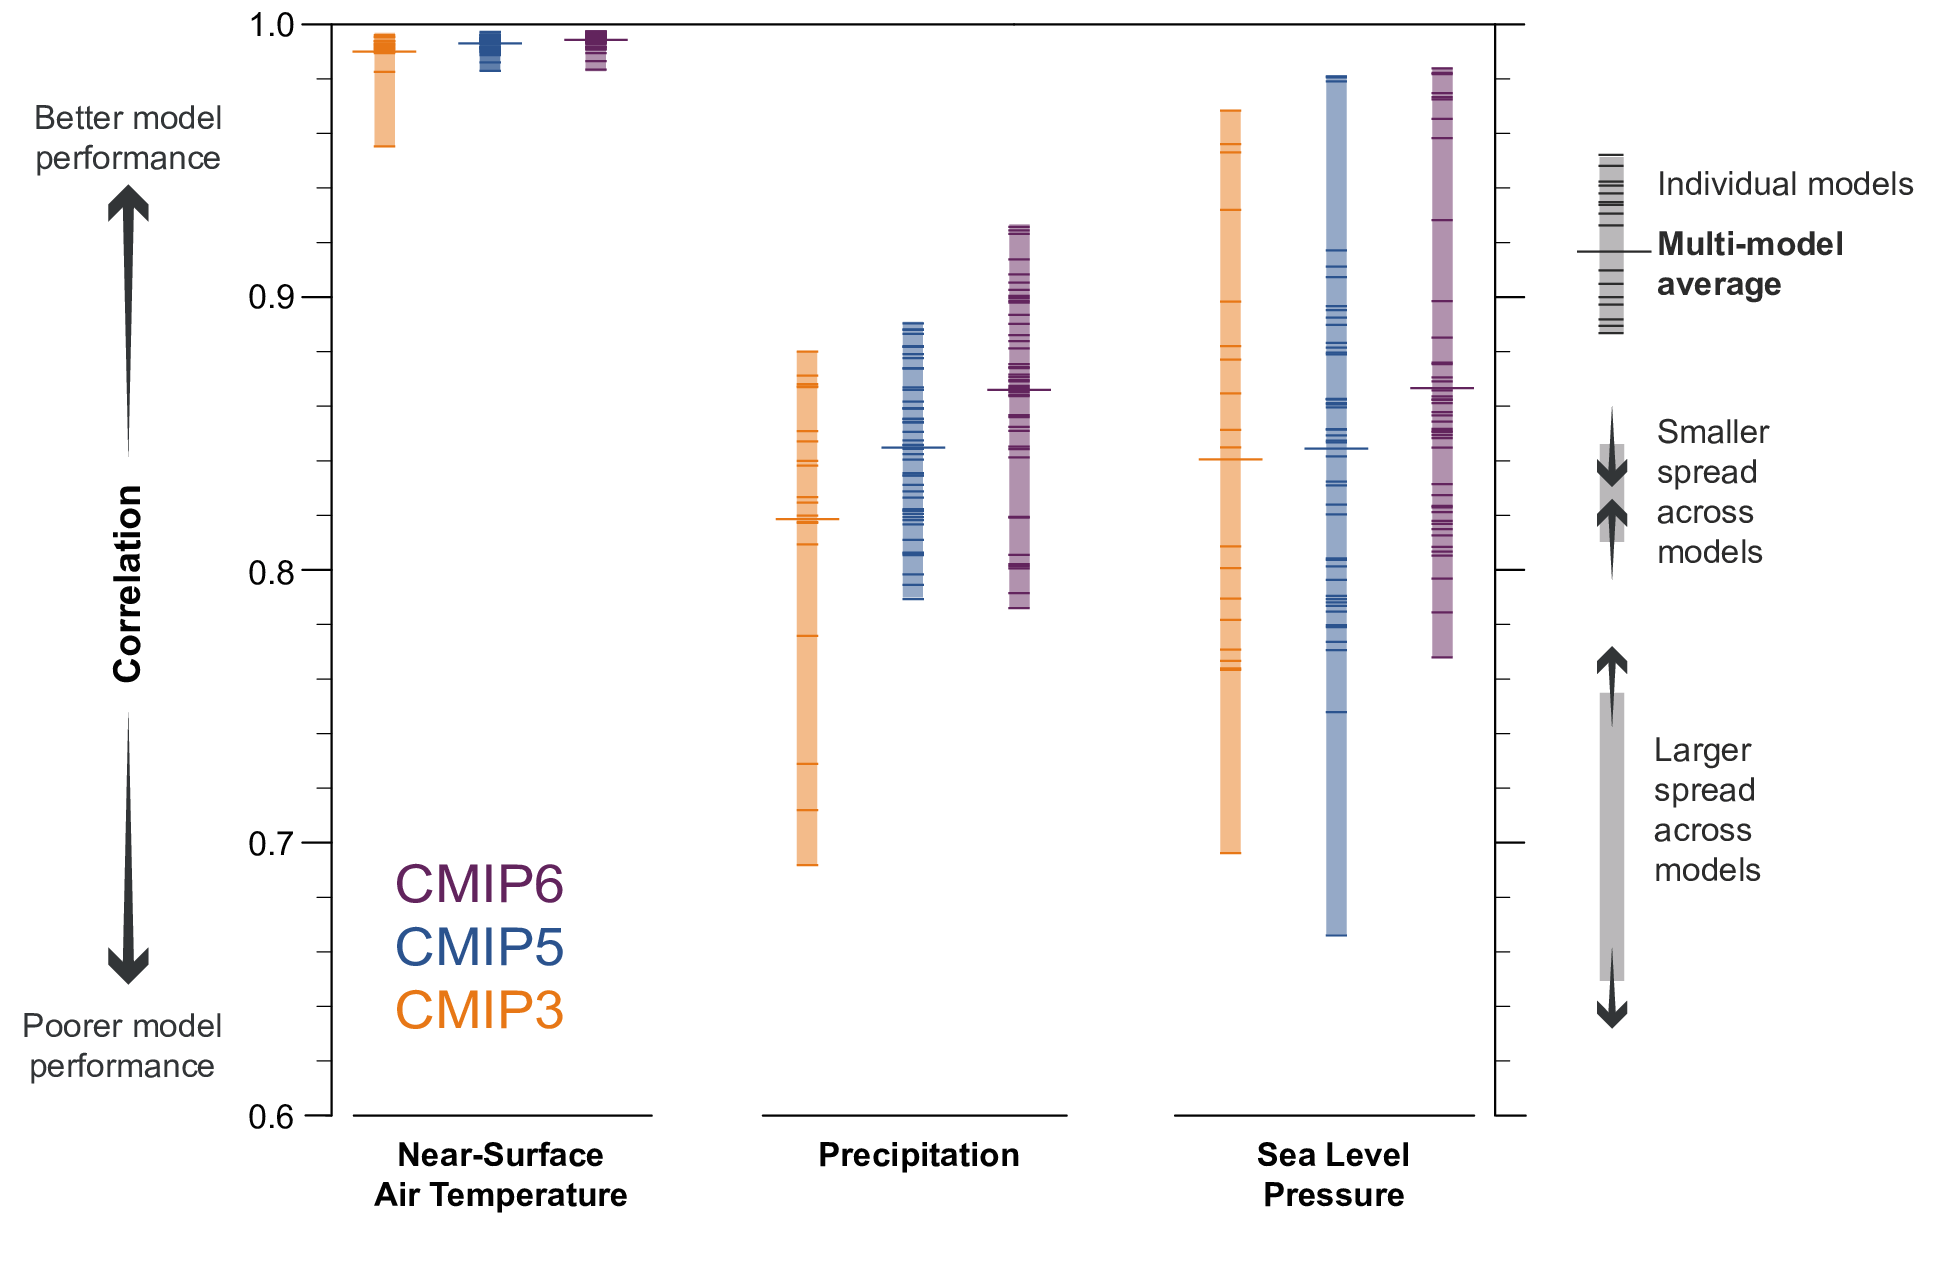
\includegraphics[width=0.7\textwidth]{figures/chapter1_figures/climate_model_accuracy.png}
    \fignote[1]{Figure from \cite{ipccAR6_model_accuracy}. The figure displays predictions for three common climate variables, near-surface air temperature, precipitation, and sea level pressure, under three different climate models. These three models are the Coupled Model Intercomparison Project Phases 3, 5, and 6. These are the three climate models used in the IPCC's fourth, fifth, and sixth assessment reports. There is no CMIP4 due to re-numbering. The vertical axis is the correlation between the model predicted outcomes the actual, observed outcomes. Clearly these models can predict near-surface air temperatures with near perfect accuracy. Other climate variables, like precipitation and sea levels rise have been more difficult to predict, but are still reasonably accurate. Climate scientists continue to learn more about the physical processes underlying climate, and consequently, these models continue to improve.
    }
\end{minipage}

\newpage
\subsection*{A.4\quad A Model of Emissions Pricing \& Environmental Inequality}

\begin{center}
    \singlespacing
    \renewcommand{\arraystretch}{1.5}
    \captionof{table}{Overview of Notation\label{notation}}
    \small
\begin{longtable}{c L{0.55\textwidth} C{0.15\textwidth} c}
    \hline\hline 
    Variable & Description & Determined & Source\\
    \hline \\[-1.8ex]
    \multicolumn{4}{l}{\emph{Indices \& Model Environment}}\\
    \hline 
    $i$ & Generator identifier & -- & -- \\
    $r$ & Region identifier & -- & -- \\
    $\ell$ & Transmission line identifier & -- & -- \\
    $m$ & Subregion or community identifier & -- & --\\ 
    $N$ & The number of generators & Exogenous & (1) \\
    $\mathcal{N}$ & Set of all generators; $\mathcal{N} = \{1, \ldots, N\}$ & Exogenous & (1) \\
    $\mathcal{N}_r$ & Set of all generators in region $r$ & Exogenous &  (1) \\
    $R$ & The number of regions & Exogenous &  (1) \\
    $\mathcal{L}$ & Set of all transmission lines & Exogenous &  (5) \\
    $M$ & Number of subregions or communities & Exogenous &  (3), (4)\\
    $T$ & Final period of the generation phase & Exogenous &  Chosen\\
    \\[-1.8ex]
    \multicolumn{4}{l}{\emph{Investment Phase}}\\
    \hline 
    $\mathcal{J}$ & Set of all investment options & Exogenous & Chosen\\
    $j_i$ & Generator $i$'s investment decision; $j_i \in \mathcal{J}$ & Endogenous & -- \\
    $j$ & Investment profile, $j = (j_1, j_2, \ldots, j_N)$ & Endogenous & -- \\
    $\rho_i^0$ & Generator $i$'s initial heat rate (BTU/kWh) & Exogenous & (1) \\
    $\rho_i$ & Generator $i$'s heat rate (BTU/kwh) & Endogenous & -- \\
    $\tilde{\delta}$ & Heat rate depreciation rate from the investment phase to the generation phase; $\tilde{\delta} \in (0, 1)$ & Exogenous & (10) \\
    $v_i$ & Generator $i$'s stochastic investment cost shock; $v_i > 0$ for all $i \in \mathcal{N}$ & Exogenous & Chosen \\
    $\gamma$ & Constant scalar in the investment cost function; $\gamma > 0$ & Exogenous & \\
    $\alpha$ & Scale parameter in the investment cost function; $\alpha > 0$ & Exogenous & \\
    $\Gamma (j_i, v_i)$ & Investment costs for generator $i$; a function of generator $i$'s investment choice $j_i$ and $i$' stochastic investment cost shock $v_i$ & Endogenous & -- \\
    $\Gamma (j \mid v)$ & Total investment costs for all generators; a function of the investment profile $j$ given a vector of all generator's stochastic investment cost shocks $v$ & Endogenous & -- \\
    $Q_t^e$ & $R$-dimensional vector of expected quantities demanded of electricity at time $t$ for each region (kWh) & Exogenous & (2)\\
    \\[-1.8ex]
    \multicolumn{4}{l}{\emph{Generation Phase}}\\
    \hline 
    $a_{it}$ & Operating decision of generator $i$ in period $t$; $a_{it} \in \{0, 1, \ldots, R\}$ where $a_{it} = r$ indicates that generator $i$ operates in period $t$ to sell its generation in region $r$ and $a_{it} = 0$ indicates that generator $i$ does not operate in period $t$ & Endogenous & -- \\
    $a_t$ & Profile of operating decisions in period $t$; $a_t = (a_{1t}, a_{2t}, \ldots, a_{Nt})$ & Endogenous & -- \\
    $\overline{q}_i$ & Generator $i$'s nameplate capacity (kW); the maximum rated generation of generator $i$ in an hour & Exogenous & (1) \\
    $q_{itr}$ & Generator $i$'s generation to be sold in region $r$'s wholesale electricity market at time $t$ (kWh) & Endogenous & -- \\
    $f_i$ & The primary fuel type of generator $i$; $f_i \in \{\text{Coal}, \text{Natural Gas}, \text{Oil}\}$ & Exogenous &  (1) \\
    $u_{f_i}$ & Unit cost of generator $i$'s fuel $f_i$ (\$/BTU) & Exogenous & (6), (7), (8)\\

    $e_{f_i}$ & Greenhouse gas emissions intensity of generator $i$'s fuel $f_i$ (tonnes CO$_2$e/BTU) & Exogenous & \\

    $\tau_r$ & Greenhouse gas emissions tax in region $r$ (\$/tonnes CO$_2$e) & Exogenous & (9) \\
    $P_{tr}$ & Price of electricity in region $r$'s wholesale market at time $t$ & Endogenous & -- \\
    $Q_{tr}$ & Quantity of electricity demanded in region $r$'s wholesale market at time $t$ & Exogenous &  (2) \\
    $C(a_t\mid j)$ & Total cost of generation in period $t$; a function of the profile if operating decisions $a_t$ given the profile of investment decisions $j$ & Endogenous & -- \\
    $MC(j)$ & Marginal cost matrix, $N \times R$; a function of the investment profile (vector) $j$; element in the $i$th row and $r$th column is $mc_{ir}$ & Endogenous & -- \\
    $G(a_t)$ & Generation matrix, $N \times R$; a function of the operating decision profile (vector) $a_t$; element in the $i$th row and $r$th column is $q_{itr}$ or $\overline{q}_i \1(a_{it} = r)$ & Endogenous & --\\
    $\rho^0$ & $N$-dimensional vector of heat rates in the absence of investment; the $i$th element is $\rho_i^0(1 + \tilde{\delta})$ & Endogenous & -- \\
    $D_{\rho^0 - j}$ & Diagonalized $N\times N$ matrix corresponding with the vector $\rho^0 - j$; for elements along the diagonal, the element in the $i$th row and $i$ column is $\rho_i = \rho_i^0(1 + \tilde{\delta}) - j_i$, all elements not along the diagonal are 0 & Endogenous & -- \\
    $U$ & Unit cost matrix, $N\times R$; the element in the $i$th row and $r$th column is generator $i$'s cost in region $r$ per BTU, $u_{f_i} + e_{f_i}\tau_r$ & Derived & -- \\
    $\overline{q}$ & $N$-dimensional vector of nameplate capacities; $\overline{q} = (\overline{q}_1, \overline{q}_2, \ldots, \overline{q}_N)$ & Derived & -- \\
    $D_{\overline{q}}$ & Diagonalized $N\times N$ matrix corresponding with the vector $\overline{q}$; for elements along the diagonal, the element in the $i$th row and $i$th column is $\overline{q}_i$, all elements not along the diagonal are 0 & Derived & -- \\
    $\1(a_t)$ & Operating decisions matrix, $N \times R$; the element in the $i$th row and $r$th column is $\1(a_{it} = r)$ & Endogenous & -- \\
    $\delta$ & Hourly discount factor, $\delta \in (0, 1)$ & Exogenous & (10)\\
    $y_{tr}$ & Net electricity exports for region $r$ at time $t$; alternatively, understood as a marginal power injection out of region $r$ at time $t$ & Endogenous & -- \\
    $PTDF_{r\ell}$ & Power transfer distribution factor on transmission line $\ell$ out of region $r$ & Exogenous & (5)\\
    $\text{Cap}_\ell$ & Maximum capacity of transmission line $\ell$ (kW) & Exogenous & (5)\\
    \\[-1.8ex]
    \multicolumn{4}{l}{\emph{The EI Gap}}\\
    \hline 
    $d$ & $M$-dimensional vector of communities' disadvantaged status; the $m$th element is 1 is $m$ is a disadvantaged community and 0 otherwise & Exogenous & (3), (4)\\
    $w$ & Local air pollutant identifier & -- & -- \\
    $e_i^w$ & Generator $i$'s emissions intensity of air pollutant $w$ (pounds/kWh) & Exogenous & (1)\\
    $w_{it}$ & Generator $i$'s emissions of air pollutant $w$ (lbs) & Endogenous & -- \\
    $\phi_w(w_{it}\mid i, t)$ & $M$-dimensional vector of the changes in the concentration of air pollutant $w$ across all $M$ communities resulting from $w_{it}$, the emissions of air pollutant $w$ from generator $i$ in time $t$ & Endogenous & -- \\
    $\Phi_w^1(T)$ & Average change in the concentration of pollutant $w$ for disadvantaged communities (elements of $d$ equal to 1) after $T$ periods & Endogenous & -- \\
    $\Phi_w^0(T)$ & Average change in the concentration of pollutant $w$ for non-disadvantaged communities (elements of $d$ equal to 0) after $T$ periods & Endogenous & -- \\
    $\text{EIGap}_w(T)$ & The environmental inequality gap after $T$ periods & Endogenous & -- \\
    \hline\hline
\end{longtable}
\fignote[1]{Table summarizes the notation used in Chapter 4. In general, lowercase letters without an index are profiles/vectors, plain-text uppercase letters denote matrices or the size of a set, and uppercase letters in the \texttt{mathcal} font are sets (e.g., $\mathcal{N}$). We denote the equilibrium of any variable as the variable with an asterisk. Derived variables are those that are a deterministic function of entirely exogenous variables. The source key for exogenous variables correspond with the data sources in Table \ref{data_sources}.}
\end{center}


\begin{center}
    \singlespacing
    \renewcommand{\arraystretch}{1.5}
    \captionof{table}{Data Sources Key\label{data_sources}}
    \small
    \begin{longtable}{c L{0.8\textwidth}}
        \hline\hline
        Source Key & Source Citation\\
        \hline \\[-3ex]
        (1) & United States Environmental Protection Agency (EPA). 2021. ``Emissions \& Generation Resource Integrated Database (eGRID), 2019" Washington, DC: Office of Atmospheric Protection, Clean Air Markets Division. Available from EPA's eGRID web site: \url{https://www.epa.gov/egrid}.\\ \\[-3ex]
        \hline \\[-3ex]
        (2) & United States Energy Information Administration (EIA). 2023. ``Hourly Electric Good Monitor'' Region Files. Available at: \url{https://www.eia.gov/electricity/gridmonitor/dashboard/electric_overview/US48/US48}\\ \\[-3ex]
        \hline \\[-3ex]
        (3) & United States Environmental Protection Agency. 2021 version. EJScreen. Census Tract-Level US Percentiles. Retrieved: 2023-03-03. Available at: \url{https://gaftp.epa.gov/EJSCREEN/2021/} \\ \\[-3ex]
        \hline \\[-3ex]
        (4) & California Office of Environmental Health \& Hazard Assessment (OEHHA). 2022. SB 535 Disadvantaged Communities. Retrieved: 2023-03-03. Available at: \url{https://oehha.ca.gov/calenviroscreen/sb535} \\ \\[-3ex]
        \hline \\[-3ex]
        (5) & Fowlie, Meredith, Petersen, Claire, and Reguant, Mar. Data and Code for: Border Carbon Adjustments When Carbon Intensity Varies Across Producers: Evidence from California. Nashville, TN: American Economic Association [publisher], 2022. Ann Arbor, MI: Inter-university Consortium for Political and Social Research [distributor], 2021-05-13. \url{https://doi.org/10.3886/E131024V1} \\ \\[-3ex]
        \hline \\[-3ex]
        (6) & United States Energy Information Administration. 2023. Natural Gas Electric Power Price. Source key: N3045. Available at: \url{http://www.eia.gov/dnav/ng/ng_pri_sum_a_epg0_peu_dmcf_m.htm} \\ \\[-3ex]
        \hline \\[-3ex]
        (7) & United States Energy Information Administration. 2023. Coal shipments to the electric power sector: price, by plant state. Available at: \url{https://www.eia.gov/coal/data/browser/} \\ \\[-3ex]
        \hline \\[-3ex]
        (8) & United States Energy Information Administration. 2023. Cushing, OK WTI Spot Price FOB (Dollars per Barrel). Source key: RWTC. Available at: \url{https://www.eia.gov/dnav/pet/hist/LeafHandler.ashx?n=PET&s=RWTC&f=M} \\ \\[-3ex]
        \hline \\[-3ex]
        (9) & California Air Resources Board. 2023. Cap-and-Trade Program Data Dashboard---Carbon Allowance Prices. Available at: \url{https://ww2.arb.ca.gov/our-work/programs/cap-and-trade-program/program-data/cap-and-trade-program-data-dashboard} \\ \\[-3ex]
        \hline \\[-3ex]
        (10) & Board of Governors of the Federal Reserve System (US), Market Yield on U.S. Treasury Securities at 10-Year Constant Maturity, Quoted on an Investment Basis [DGS10]. Retrieved: 2023-03-03 from FRED, Federal Reserve Bank of St. Louis. Available at: \url{https://fred.stlouisfed.org/series/DGS10} \\ \\[-3ex]
        \hline \\[-3ex]
        (11) & United States Energy Information Administration. 2022. Carbon Dioxide Emissions Coefficient. Available at: \url{https://www.eia.gov/environment/emissions/co2_vol_mass.php}\\ \\[-3ex]
        \hline\hline
    \end{longtable}
\end{center}

Still missing:
\begin{itemize}
    \item Investment stuff\ldots
\end{itemize}



\end{document}